%
% Template Laporan Skripsi/Thesis Universitas Indonesia
%
% @author  Ichlasul Affan, Azhar Kurnia
% @version 2.1.3
%
% Dokumen ini dibuat berdasarkan standar IEEE dalam membuat class untuk
% LaTeX dan konfigurasi LaTeX yang digunakan Fahrurrozi Rahman ketika
% membuat laporan skripsi, yang kemudian diadaptasi oleh Andreas Febrian dan
% Lia Sadita untuk template skripsi tahun 2010.
% Konfigurasi template sebelumnya telah disesuaikan dengan
% aturan penulisan thesis yang dikeluarkan UI pada tahun 2017.
%

%
% Tipe dokumen adalah report dengan satu kolom.
%
\documentclass[12pt, a4paper, onecolumn, twoside, final]{report}
\raggedbottom

% Load konfigurasi LaTeX untuk tipe laporan thesis
\usepackage[dvipsnames]{xcolor}
\usepackage{_internals/uithesis}
\usepackage{listings}
\usepackage{tabularx}
%

\definecolor{codegreen}{rgb}{0,0.6,0}
\definecolor{codegray}{rgb}{0.5,0.5,0.5}
\definecolor{codepurple}{rgb}{0.58,0,0.82}
\definecolor{backcolour}{rgb}{0.95,0.95,0.92}

\lstdefinestyle{mystyle}{
    backgroundcolor=\color{backcolour},   
    commentstyle=\color{codegreen},
    keywordstyle=\color{magenta},
    numberstyle=\tiny\color{codegray},
    stringstyle=\color{codepurple},
    basicstyle=\ttfamily\footnotesize,
    breakatwhitespace=false,         
    breaklines=true,                 
    captionpos=b,                    
    keepspaces=true,                 
    numbers=left,                    
    numbersep=5pt,                  
    showspaces=false,                
    showstringspaces=false,
    showtabs=false,                  
    tabsize=2
}

\lstset{style=mystyle}


% Load konfigurasi khusus untuk laporan yang sedang dibuat
%-----------------------------------------------------------------------------%
% Judul Dokumen
%-----------------------------------------------------------------------------%
%
% Judul laporan.
\def\judul{Sistem Tanya Jawab Bahasa Indonesia Memanfaatkan IndoNLI}
%
% Tulis kembali judul laporan namun dengan bahasa Ingris
\def\judulInggris{Indonesia's Question Answering System With Utilizing Of Indonesia Natural Language Inference (IndoNLI)}


%-----------------------------------------------------------------------------%
% Tipe Dokumen
%-----------------------------------------------------------------------------%
%
% Tipe laporan, dapat berisi: Laporan Kerja Praktik, Kampus Merdeka, Skripsi, Tugas Akhir, Thesis, atau Disertasi
\def\type{Skripsi}
%
% Nama jalur Kampus Merdeka (hanya perlu diisi jika tipe laporan adalah Kampus Merdeka
% Contoh isian (khusus Fasilkom): Studi Independen, Magang Mitra, Magang BUMN, Bangkit, Apple Academy, BYOC
\def\kampusMerdekaType{}
% Jika ada perwakilan mitra, isi dengan jabatan perwakilan mitra tersebut
% (misal: Cohort Manager)
% Kosongkan jika tidak ada perwakilan mitra
\def\partnerPosition{}
% Jika ada perwakilan mitra, isi dengan nama perusahaan atau nama program
% (misal: PT. Astra International, Bangkit Academy 2023)
% Kosongkan jika tidak ada perwakilan mitra
\def\partnerInstance{}
%
% Jenjang studi, dapat berisi: Diploma, Sarjana, Magister, atau Doktor
\def\jenjang{Sarjana}


%-----------------------------------------------------------------------------%
% Informasi Penulis
%-----------------------------------------------------------------------------%
%
% Tulis nama Anda
% Kosongkan penulisDua dan penulisTiga jika Anda melaksanakan tugas akhir/laporan secara individu
\def\penulisSatu{Muhammad Ravi Shulthan Habibi} % nama lengkap penulis pertama
\def\penulisDua{} % nama lengkap penulis kedua
\def\penulisTiga{} % nama lengkap penulis ketiga
%
% Tulis NPM Anda
% Kosongkan npmDua dan npmTiga jika Anda melaksanakan tugas akhir/laporan secara individu
\def\npmSatu{1906351000} % NPM penulis pertama
\def\npmDua{} % NPM penulis kedua
\def\npmTiga{} % NPM penulis ketiga
%
% Tulis Program Studi yang Anda ambil
% Kosongkan programDua dan programTiga jika Anda melaksanakan tugas akhir/laporan secara individu
\def\programSatu{Ilmu Komputer} % program studi penulis pertama
\def\programDua{} % program studi penulis kedua
\def\programTiga{} % program studi penulis ketiga
%
% Tulis Program Studi yang Anda ambil dalam bahasa inggris
% Kosongkan programDua dan programTiga jika Anda melaksanakan tugas akhir/laporan secara individu
\def\studyProgramSatu{Computer Science} % 1st author's study program
\def\studyProgramDua{} % 2nd author's study program
\def\studyProgramTiga{} % 3rd author's study program


%-----------------------------------------------------------------------------%
% Informasi Dosen Pembimbing & Penguji
%-----------------------------------------------------------------------------%
%
% Tuliskan pembimbing
% Untuk Kampus Merdeka: Tuliskan dosen PIC/pembimbing dari Fakultas Anda
\def\pembimbingSatu{Rahmad Mahendra, M.Sc.}
% S1 s.d. S3: Kosongkan jika tidak ada pembimbing kedua
% Untuk Kampus Merdeka: Tuliskan penanggung jawab/penyelia/mitra
%                       dari program Kampus Merdeka yang Anda ambil (jika ada)
\def\pembimbingDua{Alham Fikri Aji, Ph.D}
% S2 & S3: Kosongkan jika tidak ada pembimbing ketiga
\def\pembimbingTiga{}

%
% Tuliskan penguji
\def\pengujiSatu{Penguji Pertama Anda}
\def\pengujiDua{Penguji Kedua Anda}
% Kosongkan jika tidak ada penguji ketiga (umumnya penguji ketiga hanya ada untuk S2)
\def\pengujiTiga{}
% Kosongkan jika tidak ada penguji keempat, kelima, atau keenam (umumnya penguji > 3 hanya ada untuk S3)
\def\pengujiEmpat{}
\def\pengujiLima{}
\def\pengujiEnam{}


%-----------------------------------------------------------------------------%
% Informasi Lain (Asal Fakultas, Tanggal, dsb.)
%-----------------------------------------------------------------------------%
%
% Tuliskan Fakultas dimana penulis berada
\def\fakultas{Fakultas Ilmu Komputer}
%
% Tuliskan bulan dan tahun publikasi laporan
\Var{\bulanTahun}{Juni 2023}
%
% Tuliskan gelar yang akan diperoleh dengan menyerahkan laporan ini
\def\gelar{S.Kom}
%
% Tuliskan tanggal pengesahan laporan, waktu dimana laporan diserahkan ke
% penguji/sekretariat
\def\tanggalSiapSidang{Tanggal Bulan Tahun}
%
% Tuliskan tanggal keputusan sidang dikeluarkan dan penulis dinyatakan
% lulus/tidak lulus
\def\tanggalLulus{Tanggal Bulan Tahun}


%-----------------------------------------------------------------------------%
% Judul Setiap Bab
%-----------------------------------------------------------------------------%
%
% Berikut ada judul-judul setiap bab.
% Silahkan diubah sesuai dengan kebutuhan.
%
\Var{\kataPengantar}{Kata Pengantar}
\Var{\babSatu}{Pendahuluan}
\Var{\babDua}{Studi Literatur}
\Var{\babTiga}{Metodologi}
\Var{\babEmpat}{Implementasi Teknis}
\Var{\babLima}{Hasil dan Analisis}
\Var{\kesimpulan}{Penutup}


%-----------------------------------------------------------------------------%
% Capitalized Variables
% Anda tidak perlu mengubah apapun di bagian ini
%-----------------------------------------------------------------------------%
\Var{\Judul}{\judul}
\Var{\Type}{\type}
\Var{\PenulisSatu}{\penulisSatu}
\Var{\PenulisDua}{\penulisDua}
\Var{\PenulisTiga}{\penulisTiga}
\Var{\Fakultas}{\fakultas}
\Var{\ProgramSatu}{\programSatu}
\Var{\ProgramDua}{\programDua}
\Var{\ProgramTiga}{\programTiga}



% Daftar pemenggalan suku kata dan istilah dalam LaTeX
%
% Hyphenation untuk Indonesia
%
% @author  Andreas Febrian
% @version 2.1.2
% @edit by Ichlasul Affan, Muhammad Aulia Adil Murtito
%
% Tambahkan cara pemenggalan kata-kata yang salah dipenggal secara otomatis
% oleh LaTeX. Jika kata tersebut dapat dipenggal dengan benar, maka tidak
% perlu ditambahkan dalam berkas ini. Tanda pemenggalan kata menggunakan
% tanda '-'; contoh:
% menarik
%   --> pemenggalan: me-na-rik
%


% Silakan ganti ke bahasa Inggris (\selectlanguage{english}) jika Anda merasa terlalu banyak kata bahasa Inggris yang pemenggalannya tidak benar.
%\selectlanguage{english}


\hyphenation{
    % alphabhet A
    a-na-li-sa a-tur a-tur-an
    a-pli-ka-si
    % alphabhet B
    bab ba-ngun-an
    be-be-ra-pa
    ber-ge-rak
    ber-ke-lan-jut-an
    ber-o-per-ra-si
    ber-pe-nga-ruh
    % alphabhet C
    ca-ri Com-po-nent-UML
    % alphabhet D
    di-da-pat-kan di-sim-pan di-pim-pin di-tam-bah-kan di-tem-pat-kan de-ngan da-e-rah di-ba-ngun di-gu-na-kan da-pat di-nya-ta-kan
    di-se-mat-kan di-sim-bol-kan di-pi-lih di-li-hat de-fi-ni-si di-de-fi-ni-si-kan di-mo-del-kan di-mi-li-ki di-re-a-li-sa-si-kan di-su-sun
    % alphabhet E
    eks-pli-sit e-ner-gi en-gi-neer en-gi-neer-ing eks-klu-sif ele-men
    % alphabhet F
    fa-si-li-tas
    % alphabhet G
    ga-bung-an ge-rak ge-ne-ral ge-ne-ra-li-sa-si
    % alphabhet H
    ha-lang-an
    % alphabhet I
    in-fra-struk-tur i-ni-si-a-si
    % alphabhet J
    % alphabhet K
    ke-hi-lang-an
    ke-ter-hu-bung-an
    ku-ning
    kua-li-tas ka-me-ra ke-mung-kin-an ke-se-pa-ham-an
    % alphabhet L
    ling-kung-an
    % alphabhet M
    ma-na-je-men me-neng-ah meng-a-da-kan me-mo-ni-tor
    me-mer-lu-kan me-mo-del-kan men-de-fi-ni-si-kan meng-ak-ses me-ne-mu-kan
    meng-a-tas-i me-mo-di-fi-ka-si me-mung-kin-kan me-nge-na-i me-ngi-rim-kan meng-i-zin-kan
    meng-u-bah meng-a-dap-ta-si me-nya-ta-kan me-nyim-pan me-res-trik-si mi-cro-ser-vi-ce mi-cro-ser-vi-ces mo-di-fi-ka-si mo-dul mo-dule
    meng-a-tur meng-a-rah-kan mi-lik meng-gu-na-kan me-ne-ri-ma me-nga-la-mi
    % alphabhet N
    nya-ta non-eks-klu-sif
    % alphabhet O
    o-pe-ra-si or-ga-ni-sa-si
    % alphabhet P
	pe-nye-rap-an
	pe-ngon-trol
    pe-mo-del-an
    pe-ran  pe-ran-an-nya
    pem-ba-ngun-an pre-si-den pe-me-rin-tah pe-mi-li-han prio-ri-tas peng-am-bil-an
    peng-ga-bung-an pe-nga-was-an pe-ngem-bang-an
    pe-nga-ruh pe-nge-lo-la pa-ra-lel-is-me per-hi-tung-an per-ma-sa-lah-an
    pen-ca-ri-an pen-ce-ta-kan peng-struk-tur-an pen-ting pen-ting-nya pe-ngu-ku-ran
    pre-sen-ta-si
    % alphabhet Q
    % alphabhet R
    ran-cang-an re-fe-ren-si re-pre-sen-ta-si
    % alphabhet S
    sub-bab si-mu-la-si sa-ngat ska-la-bi-li-tas
    stan-dar-di-sa-si
    % alphabhet T
    te-ngah
    ter-da-pat
    trans-for-ma-si
    % alphabhet U
    % alphabhet V
    va-li-da-si va-ri-an va-ri-a-si va-ri-a-bi-li-tas ve-ri-fi-ka-si
    % alphabhet W
    % alphabhet X
    % alphabhet Y
    % alphabhet Z
    % special
}

% Daftar istilah yang mungkin perlu ditandai
%
% @author  Andreas Febrian
% @version 1.00
%
% Mendaftar seluruh istilah yang mungkin akan perlu dijadikan
% italic atau bold pada setiap kemunculannya dalam dokumen.
%

\var{\license}{\f{Creative Common License 1.0 Generic}}
\var{\bslash}{$\setminus$}


% Awal bagian penulisan laporan
\begin{document}
%
% Sampul Laporan
%
% Sampul Laporan

%
% @author  unknown
% @version 1.01
% @edit by Andreas Febrian
%

\begin{titlepage}
    \begin{center}
        \begin{figure}
            \begin{center}
                
\includegraphics[width=2.5cm]{assets/pics/makara_kuning.png}
            \end{center}
        \end{figure}
        \vspace*{0cm}
        \bo{
        	UNIVERSITAS INDONESIA\\
        }

        \vspace*{1.0cm}
        % judul thesis harus dalam 14pt Times New Roman
        \bo{\Judul} \\[1.0cm]

        \vspace*{2.5 cm}
        % harus dalam 14pt Times New Roman
        \bo{\Type}

		% Sesuaikan spacing agar semua informasi muat dalam satu halaman 
        \vspace*{3 cm}
        
        % penulis dan npm
        \ifx\blank\npmDua
	        \bo{\PenulisSatu} \\
	        \bo{\npmSatu} \\
        \else
	        \bo{\PenulisSatu~/ \npmSatu~/ \ProgramSatu}\\
	        \bo{\PenulisDua~/ \npmDua~/ \ProgramDua}\\
        \fi
        \ifx\blank\npmTiga\else
        	\bo{\PenulisTiga~/ \npmTiga~/ \ProgramTiga}\\
        \fi
        
        % Sesuaikan spacing agar semua informasi muat dalam satu halaman 
        \vspace*{5.0cm}

        % informasi mengenai fakultas dan program studi
        \bo{
        	FAKULTAS \Fakultas\\
        	PROGRAM STUDI \ProgramSatu \\
        	DEPOK \\
        	\bulanTahun
        }
    \end{center}
\end{titlepage}

\forceclearchapter

%
% Gunakan penomeran romawi
\pagenumbering{roman}
%
% Menghilangkan penebalan pada huruf-huruf table of content
% dari halaman judul hingga daftar lampiran
\disableboldchapterintoc
%
% load halaman judul dalam
\strcompare{Kampus Merdeka}{\type}{} {
	\addChapter{HALAMAN JUDUL}
	%
% Halaman Judul Laporan
%
% @author  unknown
% @version 1.01
% @edit by Andreas Febrian
%

\begin{titlepage}
    \begin{center}\begin{figure}
            \begin{center}
                
\includegraphics[width=2.5cm]{assets/pics/makara.png}
            \end{center}
        \end{figure}
        \vspace*{0cm}
        \bo{
        	UNIVERSITAS INDONESIA\\
        }

        \vspace*{1.0cm}
        % judul thesis harus dalam 14pt Times New Roman
        \bo{\Judul} \\[1.0cm]

        \vspace*{2.5 cm}
        % harus dalam 14pt Times New Roman
        \bo{\Type} \\
        % keterangan prasyarat
        \bo{Diajukan sebagai salah satu syarat untuk memperoleh gelar \\
        \gelar}\\

		% Sesuaikan spacing agar semua informasi muat dalam satu halaman 
        \vspace*{3 cm}
        
        % penulis dan npm
        \ifx\blank\npmDua
	        \bo{\PenulisSatu} \\
	        \bo{\npmSatu} \\
	    \else
	    	\bo{\PenulisSatu~/ \npmSatu~/ \ProgramSatu}\\
	    	\bo{\PenulisDua~/ \npmDua~/ \ProgramDua}\\
	    \fi
	    \ifx\blank\npmTiga\else
		    \bo{\PenulisTiga~/ \npmTiga~/ \ProgramTiga}\\
	    \fi
	    
		% Sesuaikan spacing agar semua informasi muat dalam satu halaman 
        \vspace*{5.0cm}

        % informasi mengenai fakultas dan program studi
        \bo{
        	FAKULTAS \Fakultas\\
        	PROGRAM STUDI \ProgramSatu \\
        	DEPOK \\
        	\bulanTahun
        }
    \end{center}
\end{titlepage}

	\forceclearchapter
}

%
% load halaman orisinalitas

% Menghilangkan penomoran
\pagenumbering{gobble}

\strcompare{Laporan Kerja Praktik}{\type}{} {
\strcompare{Kampus Merdeka}{\type}{} {
	%
% Halaman Orisinalitas
%
% @author  Andreas Febrian
% @version 2.1.2
% @edit by Muhammad Aulia Adil Murtito
%

\chapter*{\uppercase{Halaman Pernyataan Orisinalitas}}
\thispagestyle{empty}
\vspace*{2cm}

% Untuk input gambar tanda tangan, silahkan sesuaikan xshift, yshift, dan width dengan gambar tanda tangan Anda
%\begin{tikzpicture}[remember picture,overlay,shift={(current page.north east)}]
%\node[anchor=north east,xshift=-8.5cm,yshift=-14.2cm]{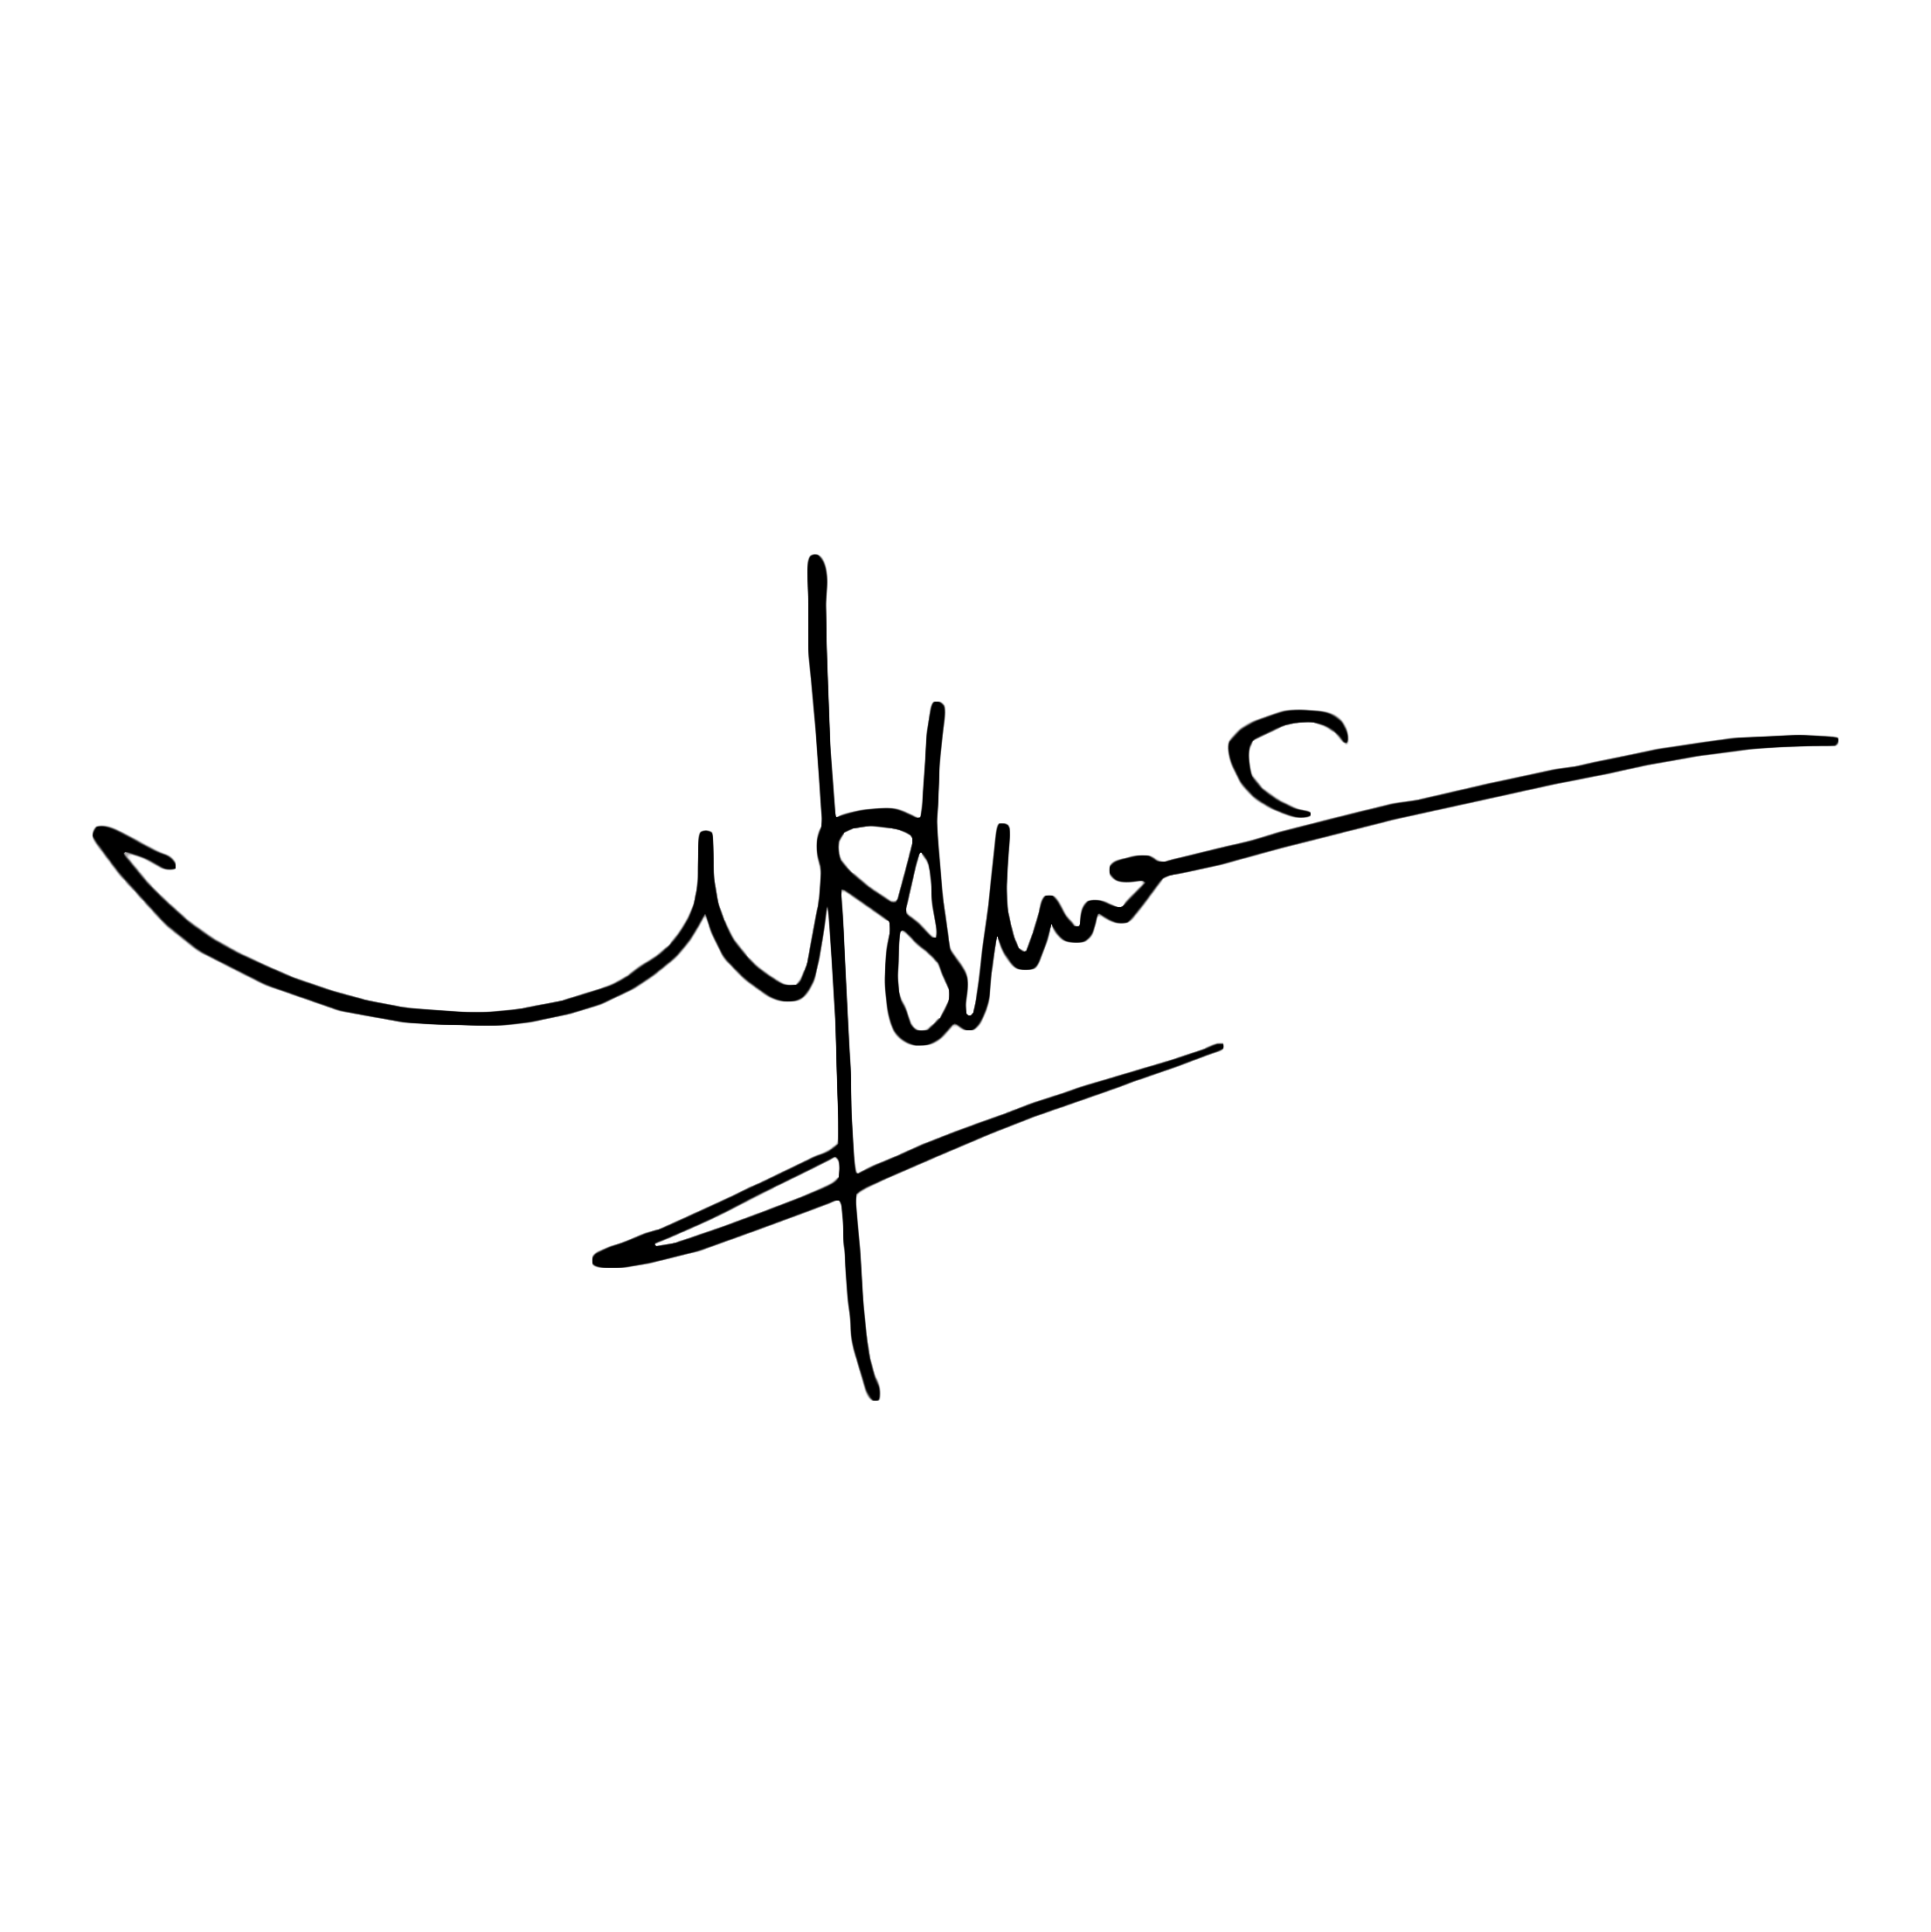
\includegraphics[width=3cm]{assets/pics/tanda_tangan_wikipedia.png}};
%\end{tikzpicture}

\begin{center}
	\bo{\type~ini adalah hasil karya saya sendiri, \\
	dan semua sumber baik yang dikutip maupun dirujuk \\
	telah saya nyatakan dengan benar.} \\
	\vspace*{2.6cm}

	\begin{tabular}{l c l}
	\ifx\blank\npmDua
	\bo{Nama} & : & \bo{\penulisSatu} \\
	\bo{NPM} & : & \bo{\npmSatu} \\
	\bo{Tanda Tangan} & : & \\
	& & \\
	& & \\
	\else
	\bo{Nama Penulis 1} & : & \bo{\penulisSatu} \\
	\bo{NPM Penulis 1} & : & \bo{\npmSatu} \\
	\bo{Tanda Tangan Penulis 1} & : & \\
	& & \\
	& & \\
	\bo{Nama Penulis 2} & : & \bo{\penulisDua} \\
	\bo{NPM Penulis 2} & : & \bo{\npmDua} \\
	\bo{Tanda Tangan Penulis 2} & : & \\
	& & \\
	& & \\
	\fi
	\ifx\blank\npmTiga\else
	\bo{Nama Penulis 3} & : & \bo{\penulisTiga} \\
	\bo{NPM Penulis 3} & : & \bo{\npmTiga} \\
	\bo{Tanda Tangan Penulis 3} & : & \\
	& & \\
	& & \\
	\fi
	\bo{Tanggal} & : & \bo{\tanggalSiapSidang} \\
	\end{tabular}
\end{center}

\newpage

	\forceclearchapter
}}

% Memunculkan penomoran kembali
\pagenumbering{roman}

%
% setelah bagian ini, halaman dihitung sebagai halaman ke 2
\setcounter{page}{2}

%
% Lembar Penegesahan
\strcompare{Laporan Kerja Praktik}{\type}
{
	% Lembar Pengesahan Kerja Praktik dari LaTeX
	\addChapter{LEMBAR PERSETUJUAN DOSEN KERJA PRAKTIK}
	%
% Halaman Pengesahan Laporan Kerja Praktik
%
% @author  Ichlasul Affan
% @version 2.1.2
% @edit by Ichlasul Affan
%

\chapter*{HALAMAN PERSETUJUAN DOSEN KERJA PRAKTIK}
\thispagestyle{empty}
\vspace*{0.4cm}
\noindent

\noindent
\begin{tabular}{ll p{9cm}}
	\multicolumn{3}{l}{\type~ini diajukan oleh:}  \\
	Nama&: & \penulisSatu \\
	NPM&: & \npmSatu \\
	Program Studi&: & \programSatu \\
	Judul Kerja Praktik&: & \judul \\
\end{tabular} \\

\vspace*{1.0cm}

\noindent \bo{Telah berhasil diselesaikan laporan kerja praktik untuk
Fakultas \fakultas~dan dipresentasikan hasil kerja praktiknya sebagai
persyaratan yang harus dipenuhi dalam mata kuliah Kerja Praktik.}\\[0.2cm]

\begin{center}
	DOSEN MATA KULIAH KERJA PRAKTIK\\[2cm]
\end{center}

\begin{center}
	\underline{\pembimbingSatu}\\[0.1cm]
\end{center}

\vspace*{2.0cm}

\begin{tabular}{ll l}
	Ditetapkan di&: & Depok\\
	Tanggal&: & \tanggalLulus \\
\end{tabular}

\newpage

	\forceclearchapter
}{
\strcompare{Kampus Merdeka}{\type}
{
	\addChapter{LEMBAR PENGESAHAN}
	%
% Halaman Pengesahan Laporan Kampus Merdeka
%
% @author  Ichlasul Affan
% @version 2.1.3
% @edit by Ichlasul Affan
%

\chapter*{LEMBAR PENGESAHAN}
\thispagestyle{empty}
\vspace*{0.4cm}
\noindent

\noindent
\begin{tabular}{ll p{9cm}}
	\multicolumn{3}{l}{Laporan Kegiatan Kampus Merdeka ini diajukan oleh:}  \\
	Nama&: & \penulisSatu \\
	NPM&: & \npmSatu \\
	Program Studi&: & \programSatu \\
	Judul Kegiatan&: & \judul \\
\end{tabular} \\

\vspace*{1.0cm}

\noindent \bo{Telah berhasil menyelesaikan program \kampusMerdekaType{} di bawah Kampus Merdeka, menyusun laporan akhir untuk Fakultas \fakultas, dan mempresentasikan hasil pekerjaannya sebagai persyaratan yang harus dipenuhi untuk melaksanakan transfer Satuan Kredit Semester (SKS) dari kegiatan tersebut.}\\[0.2cm]

\ifx\blank\pembimbingDua
	\begin{center}
		\bo{Dosen Pembimbing \kampusMerdekaType}\\
		\bo{\fakultas~Universitas Indonesia}\\[2cm]
	\end{center}
	
	\begin{center}
		\underline{\pembimbingSatu}\\[0.1cm]
	\end{center}
\else
	\begin{center}
		\begin{multicols}{2}
		\underline{\pembimbingSatu}\\[0.1cm]
		Dosen Pembimbing \kampusMerdekaType\\
		\fakultas~Universitas Indonesia\\
	
		\underline{\pembimbingDua}\\[0.1cm]
		\partnerPosition\\
		\partnerInstance\\
		\end{multicols}
	\end{center}
\fi

\vspace*{2.0cm}

\begin{tabular}{ll l}
	Ditetapkan di&: & Depok\\
	Tanggal&: & \tanggalLulus \\
\end{tabular}

\newpage

	\forceclearchapter
}
{
	\addChapter{LEMBAR PENGESAHAN}
	% Gunakan salah satu (comment atau hapus kode yang tidak perlu):
	% Lembar Pengesahan Tugas Akhir dari LaTeX
	\strcompare{Doktor}{\jenjang}
	{%
% Halaman Pengesahan Sidang (S3)
%
% @author  Andreas Febrian, Andre Tampubolon
% @version 2.1.2
% @edit by Ichlasul Affan
%

\chapter*{HALAMAN PENGESAHAN}
\thispagestyle{empty}
\vspace*{0.4cm}
\noindent

\noindent
\begin{tabular}{ll p{9cm}}
	\type~ini diajukan oleh&: & \\
	Nama&: & \penulisSatu \\
	NPM&: & \npmSatu \\
	Program Studi&: & \programSatu \\
	Judul \type&: & \judul \\
\end{tabular} \\

\vspace*{1.0cm}

\noindent \bo{Telah berhasil dipertahankan di hadapan Dewan Penguji
dan diterima sebagai bagian persyaratan yang diperlukan untuk
memperoleh gelar Doktor pada Program Studi \programSatu, Fakultas
\fakultas, Universitas Indonesia.}\\[0.2cm]

\begin{center}
	\bo{DEWAN PENGUJI}
\end{center}

\vspace*{0.3cm}

\begin{longtable}{l l p{7cm} l }
	\centering
	& & & \\
	Promotor&: & \pembimbingSatu & (\hspace*{3.0cm}) \\
	\ifx\blank\pembimbingDua
    \else
        & & & \\
    	Kopromotor&: & \pembimbingDua & (\hspace*{3.0cm}) \\
    \fi
    \ifx\blank\pembimbingTiga
    \else
        & & & \\
    	&: & \pembimbingTiga & (\hspace*{3.0cm}) \\
    \fi
	& & & \\
	Tim Penguji&: & \pengujiSatu~(Ketua) & (\hspace*{3.0cm}) \\
	& & & \\
	&: & \pengujiDua~(Anggota) & (\hspace*{3.0cm}) \\
	\ifx\blank\pengujiTiga
    \else
        & & & \\
    	&: & \pengujiTiga~(Anggota) & (\hspace*{3.0cm}) \\
    \fi
	\ifx\blank\pengujiEmpat
	\else
		& & & \\
		&: & \pengujiEmpat~(Anggota) & (\hspace*{3.0cm}) \\
	\fi
	\ifx\blank\pengujiLima
	\else
		& & & \\
		&: & \pengujiLima~(Anggota) & (\hspace*{3.0cm}) \\
	\fi
	\ifx\blank\pengujiEnam
	\else
		& & & \\
		&: & \pengujiEnam~(Anggota) & (\hspace*{3.0cm}) \\
	\fi
\end{longtable}

\vspace*{2.0cm}

\begin{tabular}{ll l}
	Ditetapkan di&: & Depok\\
	Tanggal&: & \tanggalLulus \\
\end{tabular}


\newpage
}
	{%
% Halaman Pengesahan Sidang
%
% @author  Andreas Febrian, Andre Tampubolon
% @version 2.1.2
% @edit by Muhammad Aulia Adil Murtito
%

\chapter*{HALAMAN PENGESAHAN}
\thispagestyle{empty}
\vspace*{0.4cm}

\noindent\begin{tabular}{ll p{9cm}}
	\type~ini diajukan oleh&: & \\
	\ifx\blank\npmDua
	Nama&: & \penulisSatu \\
	NPM&: & \npmSatu \\
	Program Studi&: & \programSatu\\
	\else
	\bo{Penulis 1}\\
	Nama&: & \penulisSatu \\
	NPM&: & \npmSatu \\
	Program Studi&: & \programSatu \vspace*{0.2cm}\\
	\bo{Penulis 2}\\
	Nama&: & \penulisDua \\
	NPM&: & \npmDua \\
	Program Studi&: & \programDua \vspace*{0.2cm}\\
	\fi
	\ifx\blank\npmTiga\else
	\bo{Penulis 3}\\
	Nama&: & \penulisTiga \\
	NPM&: & \npmTiga \\
	Program Studi&: & \programTiga \vspace*{0.2cm}\\
	\fi
	Judul \type&: & \judul \\
\end{tabular}

\vspace*{1.0cm}

\noindent \bo{Telah berhasil dipertahankan di hadapan Dewan Penguji
dan diterima sebagai bagian persyaratan yang diperlukan untuk
memperoleh gelar \jenjang~pada Program Studi \programSatu, Fakultas
\fakultas, Universitas Indonesia.}\\[0.2cm]

\ifx\blank\npmTiga\else\clearpage\fi

\begin{center}
	\bo{DEWAN PENGUJI}
\end{center}

\vspace*{0.3cm}

\begin{tabular}{l l p{7cm} l }
	\centering
	& & & \\
	Pembimbing 1&: & \pembimbingSatu & (\hspace*{3.0cm}) \\
	\ifx\blank\pembimbingDua
    \else
        & & & \\
    	Pembimbing 2&: & \pembimbingDua & (\hspace*{3.0cm}) \\
    \fi
	& & & \\
	Penguji 1&: & \pengujiSatu & (\hspace*{3.0cm}) \\
	& & & \\
	Penguji 2&: & \pengujiDua & (\hspace*{3.0cm}) \\
	\ifx\blank\pengujiTiga
    \else
        & & & \\
    	Penguji 3&: & \pengujiTiga & (\hspace*{3.0cm}) \\
    \fi
\end{tabular}\\

\vspace*{2.0cm}

\begin{tabular}{ll l}
	Ditetapkan di&: & Depok\\
	Tanggal&: & \tanggalLulus \\
\end{tabular}


\newpage
}
	\forceclearchapter
	% Lembar Pengesahan dari PDF lain (misal: generated oleh SISIDANG [Fasilkom])
	%\putpdf{assets/pdfs/pengesahanSidang.pdf}
}}


\strcompare{Laporan Kerja Praktik}{\type}{} {
\strcompare{Kampus Merdeka}{\type}{} {
	%
	% Kata Pengantar
	\addChapter{\kataPengantar}
	%-----------------------------------------------------------------------------%
\chapter*{\kataPengantar}
%-----------------------------------------------------------------------------%
\pagestyle{first-pages}

Template ini disediakan untuk orang-orang yang berencana menggunakan \latex~untuk membuat dokumen tugas akhir.

\todo{Silakan ganti pesan ini dengan pendahuluan kata pengantar Anda.}

Ucapan Terima Kasih:
\begin{enumerate}[topsep=0pt,itemsep=-1ex,partopsep=1ex,parsep=1ex]
	\item Pembimbing.
	\item Dosen.
	\item Instansi.
	\item Orang tua.
	\item Sahabat.
	\item Teman.
\end{enumerate}

Penulis menyadari bahwa laporan \type~ini masih jauh dari sempurna. Oleh karena itu, apabila terdapat kesalahan atau kekurangan dalam laporan ini, Penulis memohon agar kritik dan saran bisa disampaikan langsung melalui \f{e-mail} \code{emailanda@mail.id}.

\begin{figure}
	\centering
	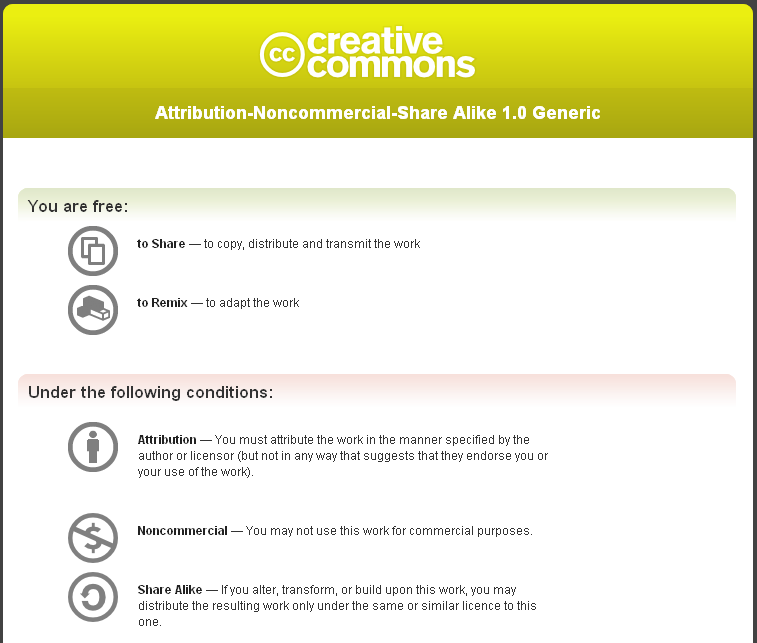
\includegraphics[width=0.74\textwidth]
	{assets/pics/creative_commons.png}
	\caption*{\license}
	\label{fig:lisensi}
\end{figure}

Terkait template ini, gambar lisensi di atas diambil dari \url{http://creativecommons.org/licenses/by-nc-sa/1.0/deed.en_CA}. Jika ingin mengentahui lebih lengkap mengenai \license, silahkan buka \url{http://creativecommons.org/licenses/by-nc-sa/1.0/legalcode}.
Seluruh dokumen yang dibuat dengan menggunakan template ini sepenuhnya menjadi hak milik pembuat dokumen dan bebas didistribusikan sesuai dengan keperluan masing-masing.
Lisensi hanya berlaku jika ada orang yang membuat template baru dengan menggunakan template ini sebagai dasarnya.

Penyusun template ingin berterima kasih kepada Andreas Febrian, Lia Sadita, Fahrurrozi Rahman, Andre Tampubolon, dan Erik Dominikus atas kontribusinya dalam template yang menjadi pendahulu template ini.
Penyusun template juga ingin mengucapkan terima kasih kepada Azhar Kurnia atas kontribusinya dalam template yang menjadi pendahulu template ini.

Semoga template ini dapat membantu orang-orang yang ingin mencoba menggunakan \latex.
Semoga template ini juga tidak berhenti disini dengan ada kontribusi dari para penggunanya.
Jika Anda memiliki perubahan yang dirasa penting untuk disertakan dalam template, silakan lakukan \f{fork} repositori Git template ini di \url{https://gitlab.com/ichlaffterlalu/latex-skripsi-ui-2017}, lalu lakukan \f{merge request} perubahan Anda terhadap \f{branch} \code{master}.
Kami berharap agar \f{template} ini dapat terus diperbarui mengikuti perubahan ketentuan dari pihak Rektorat Universitas Indonesia, dan hal itu tidak mungkin terjadi tanpa kontribusi dari teman-teman sekalian.

% Untuk input gambar tanda tangan, silahkan sesuaikan xshift, yshift, dan width dengan gambar tanda tangan Anda
%\begin{tikzpicture}[remember picture,overlay,shift={(current page.north east)}]
%\node[anchor=north east,xshift=-3cm,yshift=-6.2cm]{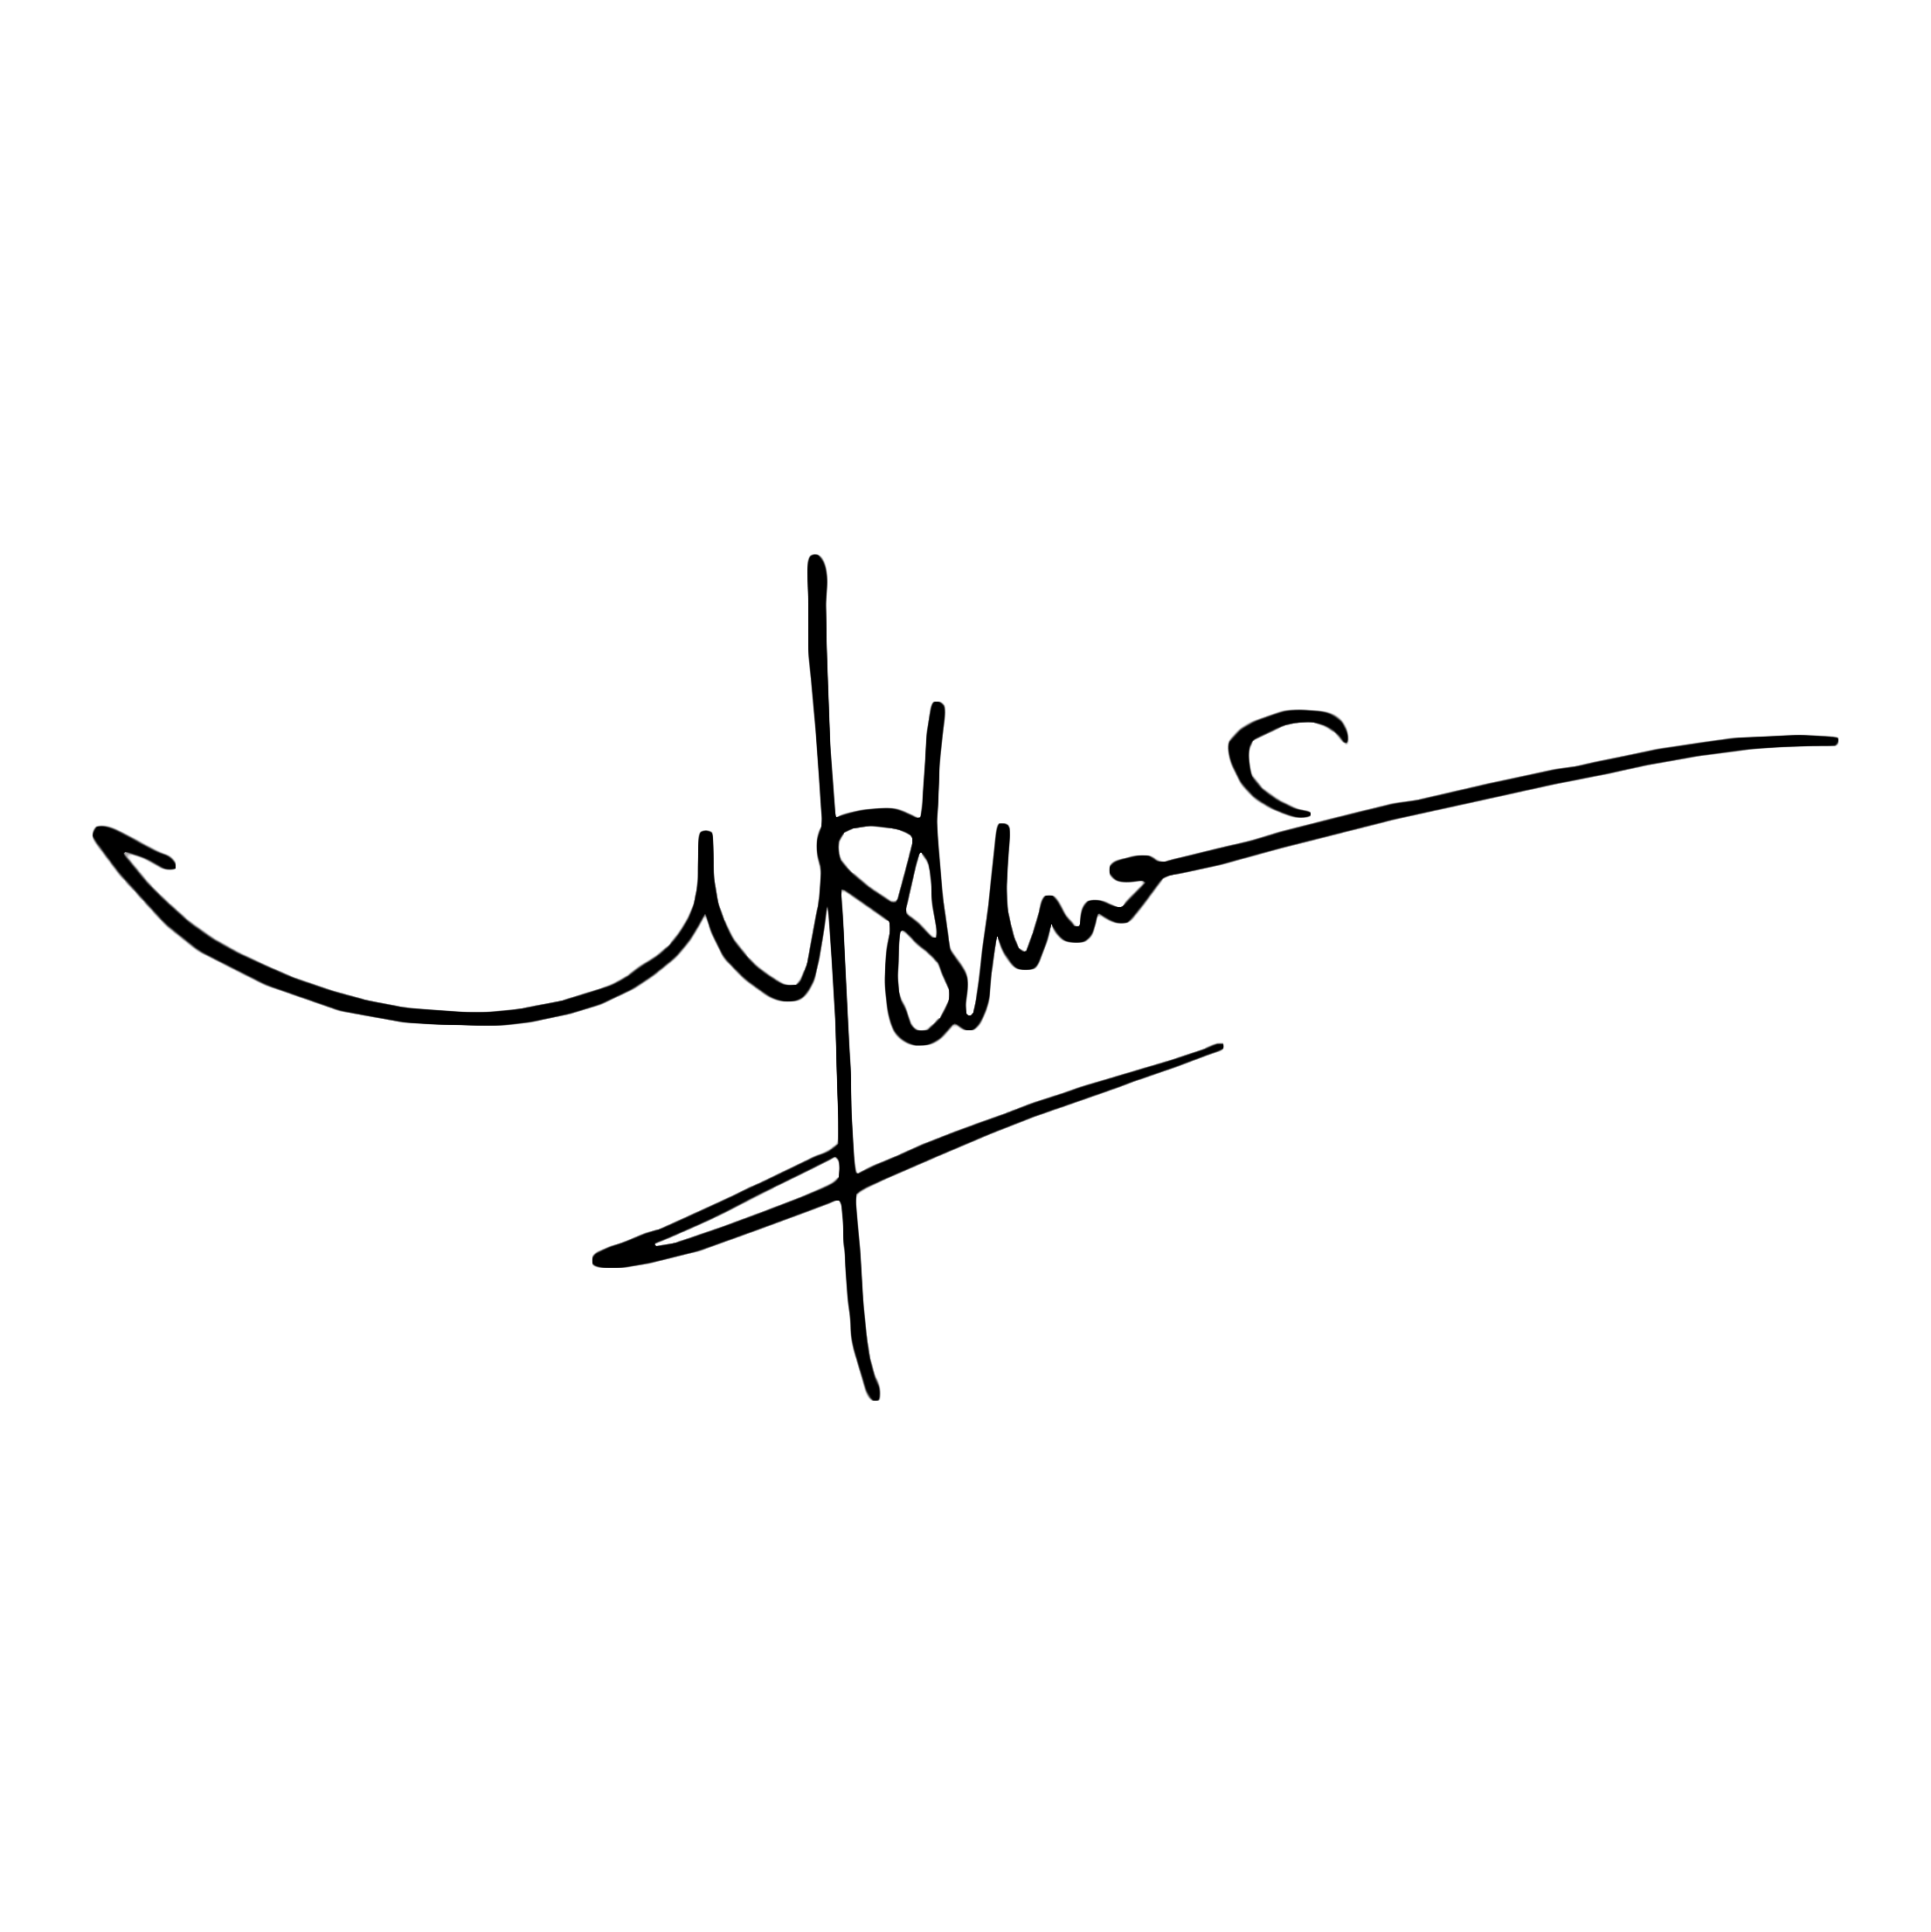
\includegraphics[width=3cm]{assets/pics/tanda_tangan_wikipedia.png}};
%\end{tikzpicture}

\vspace*{0.1cm}
\begin{flushright}
Depok, \tanggalSiapSidang\\[0.1cm]
\ifx\blank\npmDua
	\vspace*{1.5cm}
	\penulisSatu
\else
	Tim Penulis
\fi

\end{flushright}

	\forceclearchapter
	%
	% Lembar Persetujuan Publikasi Ilmiah
	\addChapter{LEMBAR PERSETUJUAN PUBLIKASI ILMIAH}
	%
% @author  Andre Tampubolon, Andreas Febrian
% @version 2.1.2
% @edit by Muhammad Aulia Adil Murtito
%

\chapter*{\uppercase{Halaman Pernyataan Persetujuan Publikasi Tugas Akhir untuk Kepentingan Akademis}}
\thispagestyle{empty}
\noindent
Sebagai sivitas akademik Universitas Indonesia, \ifx\blank\npmDua{saya}\else{kami}\fi~yang bertanda
tangan di bawah ini:

\vspace*{0.2cm}

\begin{tabular}{p{4.2cm} l p{6.5cm}}
	\ifx\blank\npmDua
	Nama&: & \penulisSatu \\
	NPM&: & \npmSatu \\
	Program Studi&: & \programSatu\\
	\else
	\bo{Penulis 1}\\
	Nama&: & \penulisSatu \\
	NPM&: & \npmSatu \\
	Program Studi&: & \programSatu \vspace*{0.1cm}\\
	\bo{Penulis 2}\\
	Nama&: & \penulisDua \\
	NPM&: & \npmDua \\
	Program Studi&: & \programDua \vspace*{0.1cm}\\
	\fi
	\ifx\blank\npmTiga\else
	\bo{Penulis 3}\\
	Nama&: & \penulisTiga \\
	NPM&: & \npmTiga \\
	Program Studi&: & \programTiga \vspace*{0.1cm}\\
	\fi
	\bo{Jenis Karya} & : & \type \\
\end{tabular}

\vspace*{0.2cm}

\noindent demi pengembangan ilmu pengetahuan, menyetujui untuk memberikan
kepada Universitas Indonesia \bo{Hak Bebas Royalti Noneksklusif
(\textit{Non-exclusive Royalty Free Right})} atas karya ilmiah saya yang berjudul:
\begin{center}
	\judul
\end{center}
beserta perangkat yang ada (jika diperlukan). Dengan Hak Bebas Royalti
Noneksklusif ini Universitas Indonesia berhak menyimpan,
mengalihmedia/formatkan, mengelola dalam bentuk pangkalan data
(\textit{database}), merawat, dan memublikasikan tugas akhir saya selama
tetap mencantumkan nama saya sebagai penulis/pencipta dan sebagai
pemilik Hak Cipta. \\

\noindent Demikian pernyataan ini saya buat dengan sebenarnya.

\ifx\blank\npmDua\else\clearpage\fi

% Untuk input gambar tanda tangan, silahkan sesuaikan xshift, yshift, dan width dengan gambar tanda tangan Anda
%\begin{tikzpicture}[remember picture,overlay,shift={(current page.north east)}]
%\node[anchor=north east,xshift=-9cm,yshift=-23.5cm]{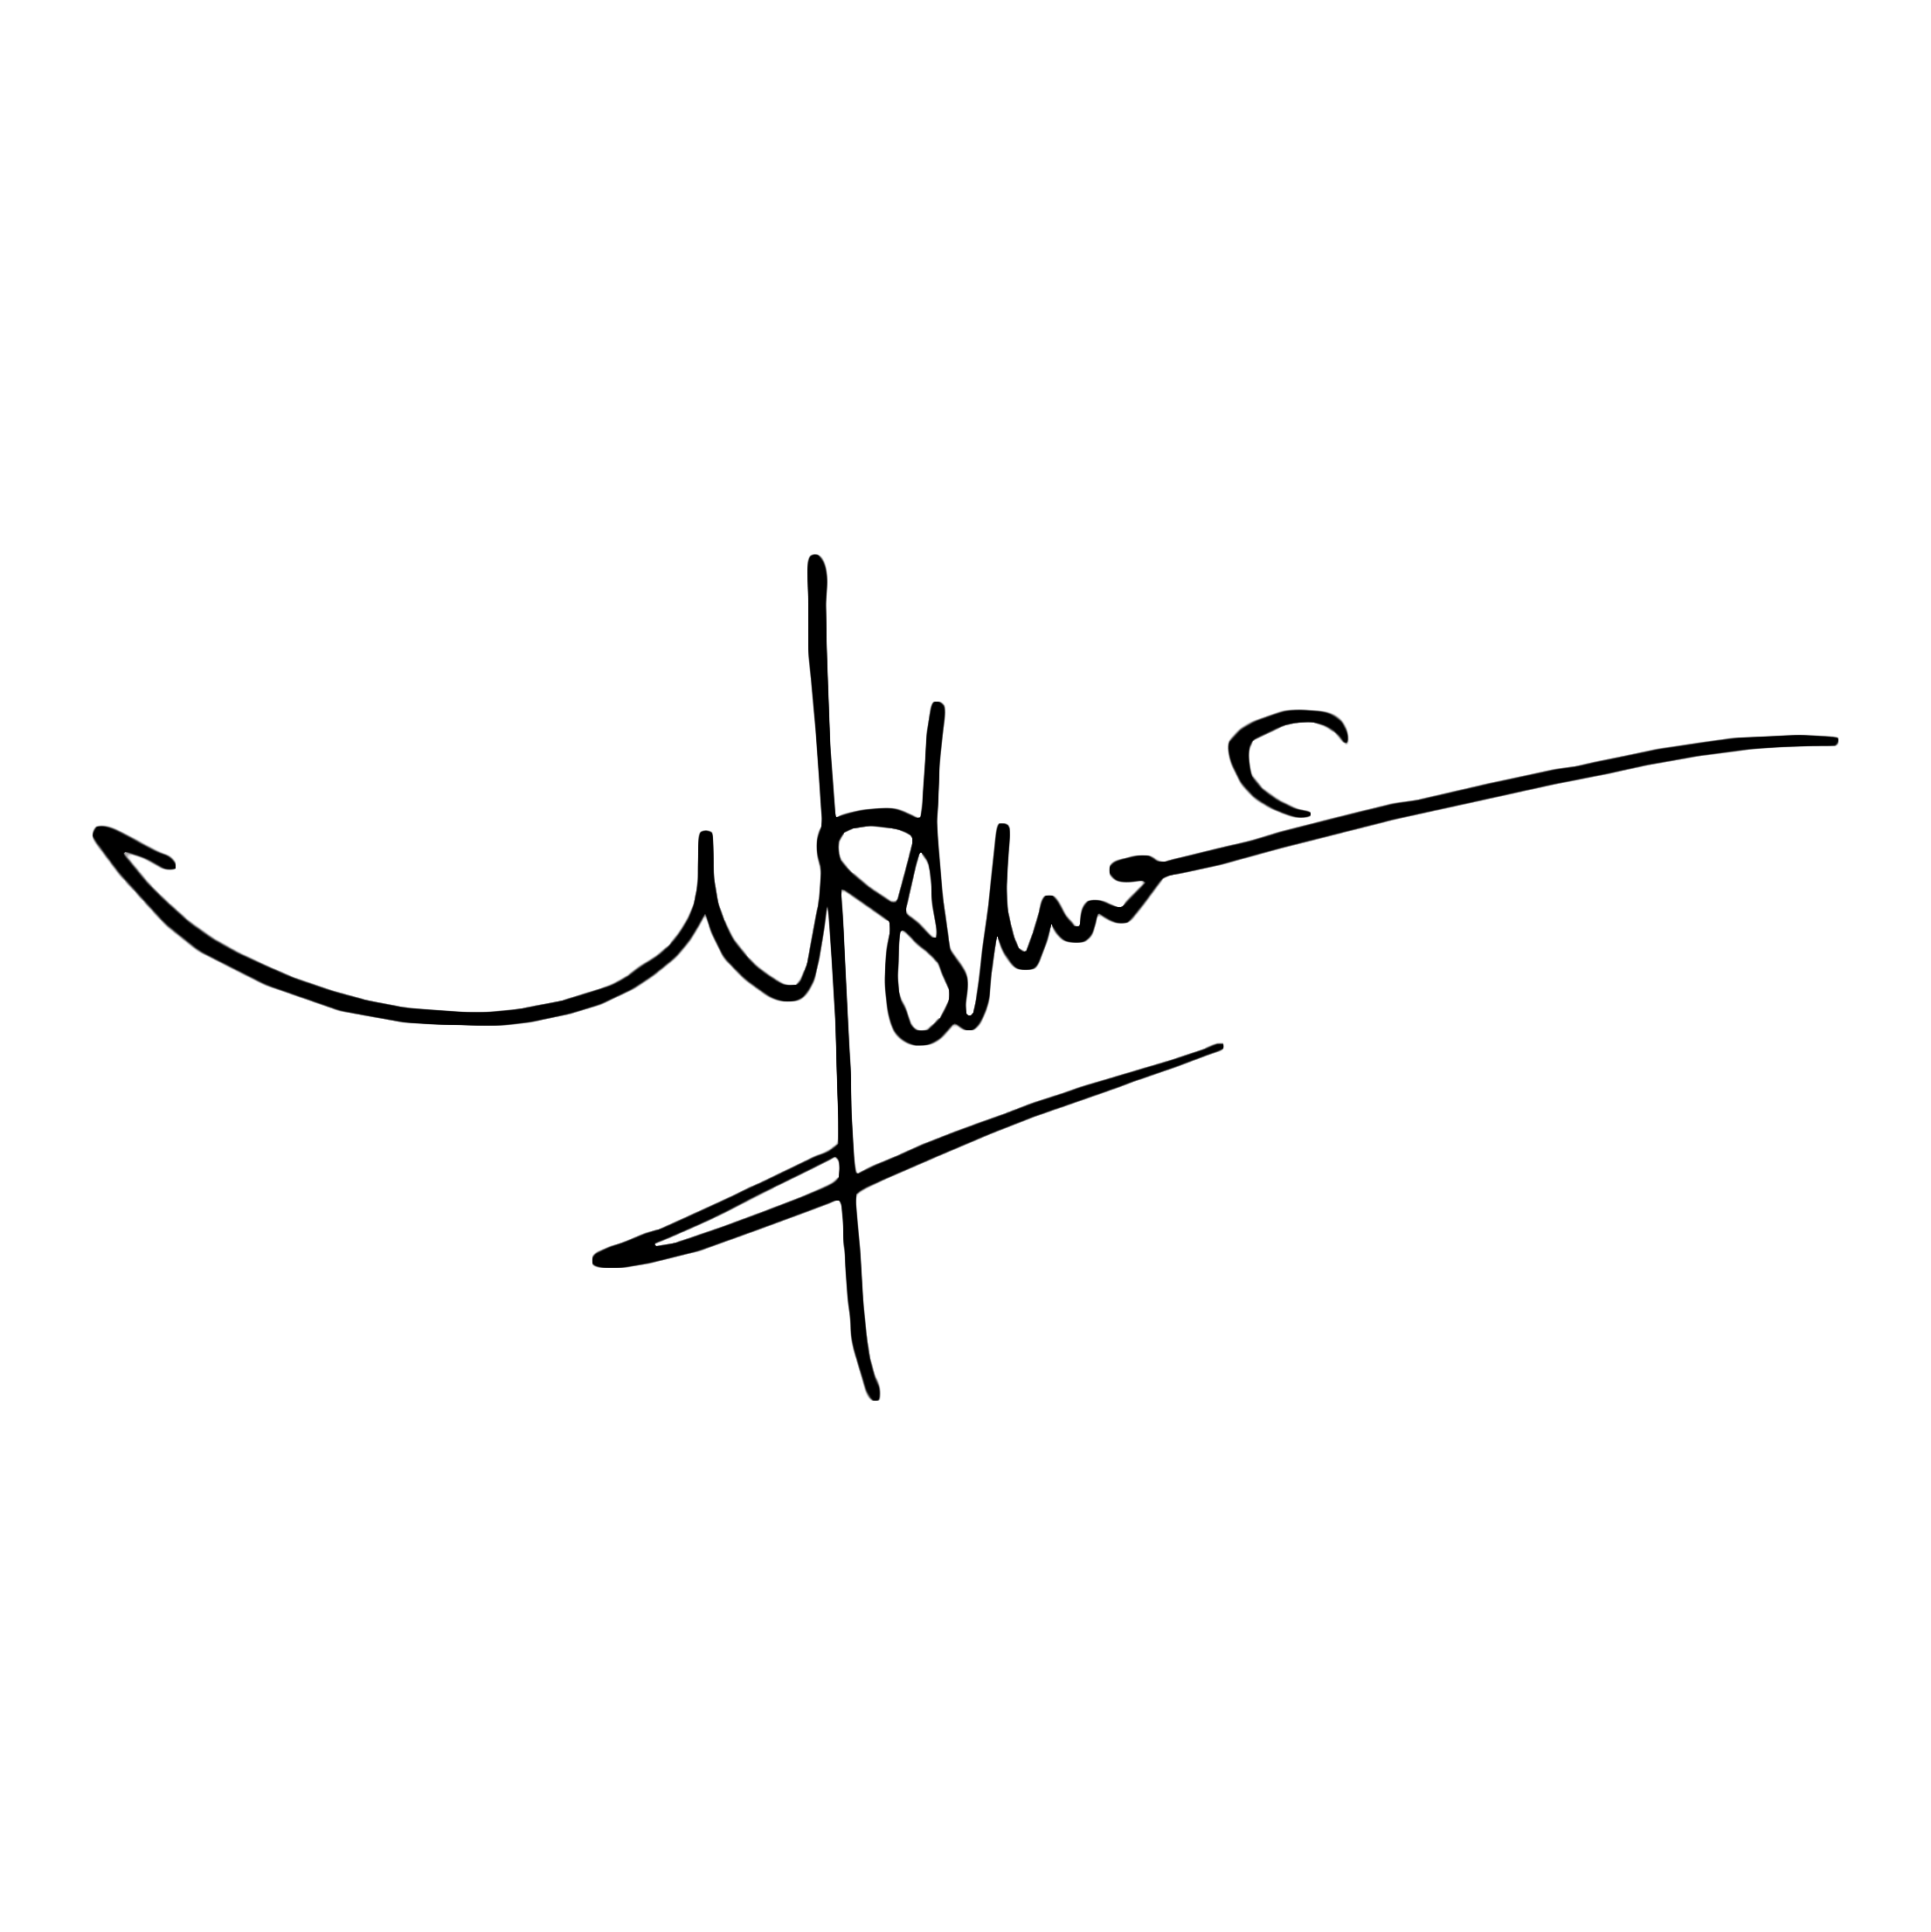
\includegraphics[width=3cm]{assets/pics/tanda_tangan_wikipedia.png}};
%\end{tikzpicture}


\begin{center}
	\vspace*{0.8cm}
	\begin{tabular}{lll}
		Dibuat di&: & Depok \\
		Pada tanggal&: & \tanggalSiapSidang \\
	\end{tabular}\\

	\vspace*{0.2cm}
	Yang menyatakan \\
	\ifx\blank\npmDua
		\vspace*{2cm}
		(\penulisSatu)
	\else
		\begin{multicols}{2}
			Penulis 1:\\
			\vspace*{2cm}
			(\penulisSatu)\\
			
			Penulis 2:\\
			\vspace*{2cm}
			(\penulisDua)\\
		\end{multicols}
	\fi
	\ifx\blank\npmTiga\else
		\vspace*{0.2cm}
		Penulis 3:\\
		\vspace*{2cm}
		(\penulisTiga)
	\fi
\end{center}

\newpage

	\forceclearchapter
}}

%
% Untuk halaman pertama setiap chapter mulai dari abstrak, tetap berikan mark universitas.
%
\pagestyle{first-pages}

%
\addChapter{ABSTRAK}
%
% Halaman Abstrak
%
% @author  Andreas Febrian
% @version 2.1.2
% @edit by Ichlasul Affan
%

\chapter*{Abstrak}
\singlespacing

\vspace*{0.2cm}

\noindent \begin{tabular}{l l p{10cm}}
	\ifx\blank\npmDua
		Nama&: & \penulisSatu \\
		Program Studi&: & \programSatu \\
	\else
		Nama Penulis 1 / Program Studi&: & \penulisSatu~/ \programSatu\\
		Nama Penulis 2 / Program Studi&: & \penulisDua~/ \programDua\\
	\fi
	\ifx\blank\npmTiga\else
		Nama Penulis 3 / Program Studi&: & \penulisTiga~/ \programTiga\\
	\fi
	Judul&: & \judul \\
	Pembimbing&: & \pembimbingSatu \\
	\ifx\blank\pembimbingDua
    \else
        \ &\ & \pembimbingDua \\
    \fi
    \ifx\blank\pembimbingTiga
    \else
    	\ &\ & \pembimbingTiga \\
    \fi
\end{tabular} \\

\vspace*{0.5cm}

\noindent Isi abstrak. \\

\vspace*{0.2cm}

\noindent Kata kunci: \\ \f{Keyword} satu, kata kunci dua \\

\setstretch{1.4}
\newpage

%
%
%
% Halaman Abstract
%
% @author  Andreas Febrian
% @version 2.1.2
% @edit by Ichlasul Affan
%

\chapter*{ABSTRACT}
\singlespacing

\vspace*{0.2cm}

\noindent \begin{tabular}{l l p{11.0cm}}
	\ifx\blank\npmDua
		Name&: & \penulisSatu \\
		Study Program&: & \studyProgramSatu \\
	\else
		Writer 1 / Study Program&: & \penulisSatu~/ \studyProgramSatu\\
		Writer 2 / Study Program&: & \penulisDua~/ \studyProgramDua\\
	\fi
	\ifx\blank\npmTiga\else
		Writer 3 / Study Program&: & \penulisTiga~/ \studyProgramTiga\\
	\fi
	Title&: & \judulInggris \\
	Counselor&: & \pembimbingSatu \\
	\ifx\blank\pembimbingDua
	\else
		\ &\ & \pembimbingDua \\
	\fi
	\ifx\blank\pembimbingTiga
	\else
		\ &\ & \pembimbingTiga \\
	\fi
\end{tabular} \\

\vspace*{0.5cm}

\noindent Abstract content. \\

\vspace*{0.2cm}

\noindent Key words: \\ Keyword one, keyword two \\

\setstretch{1.4}
\newpage


%
% Daftar isi, gambar, tabel, dan kode
%
\CAPinToC % All entries in ToC will be CAPITALIZED from here on
\phantomsection %hack to make them clickable
\singlespacing
\tableofcontents
\setstretch{1.4}
\clearpage
\phantomsection %hack to make them clickable
\singlespacing
\listoffigures
\setstretch{1.4}
\clearpage
\phantomsection %hack to make them clickable
\singlespacing
\listoftables
\setstretch{1.4}
\clearpage

%
% Daftar Kode Program
% Comment to disable.
%
\phantomsection %hack to make them clickable
\addcontentsline{toc}{chapter}{\lstlistlistingname}
\singlespacing
\listoflistings
\setstretch{1.4}
\clearpage

%
% Daftar Isi yang Didefinisikan Sendiri (Custom)
% Definisi jenis objek baru dapat dilakukan di uithesis.sty
% Uncomment to use.
%
%\phantomsection %hack to make them clickable
%\addcontentsline{toc}{chapter}{\listofthingname}
%\singlespacing
%\listofthing
%\setstretch{1.4}
%\clearpage

%
% Daftar Equation (Persamaan Matematis)
% Uncomment to use.
%
% \phantomsection %hack to make them clickable
% \addcontentsline{toc}{chapter}{\listofequname}
% \singlespacing
% \listofequ
% \setstretch{1.4}
% \clearpage

%
% Daftar Lampiran
% Comment to disable.
%
\phantomsection %hack to make them clickable
\addcontentsline{toc}{chapter}{\listofappendixname}
\singlespacing
\listofappendix
\setstretch{1.4}

% Table of content normal lagi hurufnya
\enableboldchapterintoc

\clearpage

% Jika penomoran romawi selesai di ganjil
%\naiveoddclearchapter
% Jika penomoran romawi selesai di genap
%\naiveevenclearchapter

\noCAPinToC % Revert to original \addcontentsline formatting

%
% Gunakan penomeran Arab (1, 2, 3, ...) setelah bagian ini.
%
\pagenumbering{arabic}
\pagestyle{standard}
% \setlength{\belowcaptionskip}{+2pt}


\setoddevenheader
%-----------------------------------------------------------------------------%
\chapter{\babSatu}
\label{bab:1}
%-----------------------------------------------------------------------------%
Bab pertama ini menjelaskan mengenai pendahuluan penelitian yang telah penulis rancang untuk penelitian ini. Sub-bab 1.1 menjelaskan mengenai latar belakang penelitian. Sub-bab 1.2 menjelaskan mengenai rumusan masalah yang akan dipecahkan pada penelitian ini. Sub-bab 1.3 menjelaskan tentang tujuan penelitian. Sub-bab 1.4 menjelaskan tentang manfaat penelitian. Sub-bab 1.4 menjelaskan tentang ruang lingkup dan limitasi dari penelitian ini. Sub-bab 1.6 menjelaskan tentang sistematika penulisan laporan penelitian ini.

%-----------------------------------------------------------------------------%
\section{Latar Belakang}
\label{sec:latarBelakang}
%-----------------------------------------------------------------------------%
Sistem tanya jawab (\emph{question answering}) merupakan suatu permasalahan pada domain \emph{natural language processing} (NLP), sederhananya permasalahan sistem tanya jawab adalah suatu task di mana mesin akan belajar untuk menjawab pertanyaan yang diberikan oleh pengguna berdasarkan konteks yang ada (Stroh \& Mathur, n.d.). Sehingga, dapat disimpulkan bahwa masukan dari \emph{task} ini adalah pertanyaan dan konteks; dan keluarannya adalah jawaban berdasarkan pertanyaan dan konteks yang diberikan sebelumnya. Pada \emph{task} sistem tanya jawab, kita dapat meningkatkan performa model dengan berbagai macam metode, salah satunya dengan memanfaatkan \emph{natural language inference} (NLI). NLI merupakan suatu \emph{semantic task} pada domain NLP yang bertujuan untuk mengkarakterisasi dan memanfaatkan relasi antar dua kalimat, untuk menyelesaikan hal tersebut, model membutuhkan kemampuan untuk mengurai semantik kalimat dan penalaran logis (\emph{commonsense}) yang baik \citep{bowman-etal-2015-large}. Sebenarnya, model sistem tanya jawab sudah banyak ditemui dengan berbasis bahasa Inggris, namun masih sedikit model sistem tanya jawab berbasis bahasa Indonesia dan juga performa model sistem tanya jawab berbahasa Indonesia masih kurang baik.


Berdasarkan uraian pada di atas, penulis berusaha untuk mengembangkan model sistem tanya jawab berbahasa Indonesia dengan memanfaatkan model IndoNLI sebagai media penyelesaian jawaban, verifikator jawaban, dan peningkatan performa model sistem tanya jawab itu sendiri. IndoNLI merupakan dataset NLI berbahasa Indonesia (Mahendra, et.al, 2021). Pemanfaatan IndoNLI pada sistem sistem tanya jawab berbahasa Indonesia rencananya akan menggunakan dua metode, yaitu: \emph{intermediate pre-training} dan \emph{task recasting}. \emph{Intermediate pre-training} merupakan teknik peningkatan performa dengan melakukan \emph{pre-training} dengan \emph{dataset} IndoNLI pada model BERT \emph{baseline}, lalu model tersebut akan dilakukan \emph{fine-tuning} untuk \emph{task} sistem tanya jawab-nya. Sedangkan \emph{task recasting} merupakan teknik peningkatan performa dengan melakukan \emph{recasting input} \& \emph{output} sistem tanya jawab menjadi \emph{input \& output task} NLI atau sebaliknya, hal tersebut dilakukan dalam rangka validasi hasil prediksi jawaban dari sistem tanya jawab maupun sebagai penghasil jawaban dari dataset IndoNLI. Harapan penulis, dengan memanfaatkan IndoNLI, performa sistem tanya jawab berbahasa Indonesia dapat meningkat dibanding sistem tanya jawab sebelumnya yang tidak memanfaatkan IndoNLI.


%-----------------------------------------------------------------------------%
\section{Permasalahan}
\label{sec:masalah}
%-----------------------------------------------------------------------------%
\noindent\todo{Sebutkan permasalahan penelitian Anda dari latar belakang tersebut.}

%-----------------------------------------------------------------------------%
\subsection{Definisi Permasalahan}
\label{sec:definisiMasalah}
%-----------------------------------------------------------------------------%
Berikut ini adalah rumusan permasalahan dari penelitian yang dilakukan:
\begin{itemize}
	\item Bagaimana cara membuat pertanyaan penelitian?
\end{itemize}
\noindent\todo{Tuliskan permasalahan yang ingin diselesaikan. Bisa juga berbentuk pertanyaan}

%-----------------------------------------------------------------------------%
\subsection{Batasan Permasalahan}
\label{sec:batasanMasalah}
%-----------------------------------------------------------------------------%
Berikut ini adalah asumsi yang digunakan sebagai batasan penelitian ini:
\begin{itemize}
	\item Salah satu batasannya adalah, ini hanya \f{template}.
\end{itemize}

\noindent\todo{Umumnya ada asumsi atau batasan yang digunakan untuk menjawab pertanyaan-pertanyaan penelitian diatas.}


%-----------------------------------------------------------------------------%
\section{Tujuan Penelitian}
\label{sec:tujuan}
%-----------------------------------------------------------------------------%
Berikut ini adalah tujuan penelitian yang dilakukan:
\begin{itemize}
	\item Untuk memberikan \f{template} yang dapat mempermudah skripsi orang lain.
\end{itemize}

\noindent\todo{Tuliskan tujuan penelitian Anda di bagian ini.}


%-----------------------------------------------------------------------------%
\section{Posisi Penelitian}
\label{sec:posisiPenelitian}
%-----------------------------------------------------------------------------%
\todo{
	Sebutkan posisi penelitian Anda. Ada baiknya jika Anda menggunakan gambar atau diagram.
	Template ini telah menyediakan contoh cara memasukkan gambar.
	}

\begin{figure}
	\centering
	
\includegraphics[width=0.4\textwidth]{assets/pics/makara.png}
	\caption{Penjelasan singkat terkait gambar.}
	\label{fig:research_position}
\end{figure}

\noindent\todo{Jelaskan \pic~\ref{fig:research_position} di sini.}


%-----------------------------------------------------------------------------%
\section{Langkah Penelitian}
\label{sec:langkahPenelitian}
%-----------------------------------------------------------------------------%
Berikut ini adalah langkah penelitian yang telah dilakukan:
\begin{enumerate}
	\item Tinjauan literatur \\
	Pada tahap ini, dipelajari teori-teori yang terkait dengan penelitian ini untuk mendapatkan konsep dasar yang dibutuhkan dalam mencapai tujuan penelitian.
	\item Analisis implementasi dan kesimpulan \\
	Pada tahap ini, digunakan studi kasus untuk analisis terkait kegunaan \f{template}.
	Setelah melakukan analisis tersebut, ditarik kesimpulan keseluruhan dari penelitian ini.
\end{enumerate}


%-----------------------------------------------------------------------------%
\section{Sistematika Penulisan}
\label{sec:sistematikaPenulisan}
%-----------------------------------------------------------------------------%
Sistematika penulisan laporan adalah sebagai berikut:
\begin{itemize}
	\item Bab 1 \babSatu \\
	    Bab ini mencakup latar belakang, cakupan penelitian, dan pendefinisian masalah.
	\item Bab 2 \babDua \\
	    Bab ini mencakup pemaparan terminologi dan teori yang terkait dengan penelitian berdasarkan hasil tinjauan pustaka yang telah digunakan, sekaligus memperlihatkan kaitan teori dengan penelitian.
	\item Bab 3 \babTiga \\
	    Apa itu Bab 3?
	\item Bab 4 \babEmpat \\
		Apa itu Bab 4?
	\item Bab 5 \babLima \\
	    Apa itu Bab 5?
	\item Bab 6 \kesimpulan \\
	    Bab ini mencakup kesimpulan akhir penelitian dan saran untuk pengembangan berikutnya.
\end{itemize}

\noindent\todo{Anda bisa mengubah atau menambahkan penjelasan singkat mengenai isi masing-masing bab. Setiap tugas akhir pasti ada yang berbeda pada bagian ini.}

\clearchapter
%-----------------------------------------------------------------------------%
\chapter{\babDua}
\label{bab:2}
%-----------------------------------------------------------------------------%
Bab kedua ini menjelaskan mengenai studi literatur yang telah penulis telusuri dan kaji untuk penelitian ini. Sub-bab \ref{2.1} menjelaskan mengenai sistem tanya jawab, \emph{question answering task}, bidang khusus yang menjadi domain penelitian ini. Sub-bab \ref{2.2} menjelaskan tentang \emph{dataset} sistem tanya jawab, \emph{dataset} tersebut ada yang berbahasa Indonesia maupun berbahasa Inggris. Sub-bab \ref{2.3} menjelaskan tentang \emph{natural language inference}, salah satu alat (\emph{tools}) eksperimen untuk meningkatkan performa dari sistem tanya jawab dan \emph{dataset} NLI berbahasa Indonesia yang digunakan, yaitu: IndoNLI. Sub-bab \ref{2.4} menjelaskan tentang \emph{transformer}, salah satu arsitektur model kecerdasan buatan terbaru untuk dapat memprediksi jawaban. Sub-bab \ref{2.5} menjelaskan tentang \emph{pre-trained language model} yang digunakan pada penelitian ini. Sub-bab \ref{2.6} dan sub-bab \ref{2.7} menjelaskan tentang \emph{intermediate-task transfer learning} dan \emph{task recasting}, yaitu metode-metode eksperimen yang akan dilakukan pada penelitian ini. Terakhir, sub-bab \ref{2.8} menjelaskan tentang metrik evaluasi yang digunakan pada penelitian ini.

%-----------------------------------------------------------------------------%
\section{Sistem Tanya Jawab (\emph{Question Answering System})}
\label{2.1}
%-----------------------------------------------------------------------------%

\begin{figure}[h]
\vspace{3pt}
\hrule
\vspace{3pt}

\textbf{\emph{Context}}: Otranto adalah kota dan komune yang terletak di  \colorbox{BurntOrange}{provinsi Lecce} (\colorbox{ForestGreen}{Apulia, Italia}). Otranto berada di pantai timur semenanjung Salento. Selat Otranto menghubungkan Laut Adriatik dengan Laut Ionia. Pelabuhan kota ini kecil dan terdapat sedikit perdagangan.\\

\textbf{\emph{Question}}: \colorbox{BurntOrange}{Dimanakah letak Lecce ?}\\

\textbf{\emph{Answer}}:  \colorbox{ForestGreen}{Apulia, Italia}

\vspace{3pt}
\hrule
\vspace{3pt}
\centering
\caption{Contoh dari \emph{question answering task} dari data \citep{putri-oh-2022-idk}.}
\end{figure}

Sistem tanya jawab merupakan salah satu tugas (\emph{task}) dari domain \emph{Natural Language Processing} (NLP). Sistem tanya jawab adalah sistem yang dirancang untuk memenuhi kebutuhan informasi manusia yang mungkin muncul dalam situasi seperti berbicara dengan asisten virtual, berinteraksi dengan pencarian mesin (\emph{search engine}), atau sekedar menanyakan data di basis data (\emph{database}) saja \citep{daniel2007speech}. Salah satu paradigma pencarian jawaban dari suatu sistem tanya jawab ini adalah dengan berbasis pencarian informasi (\emph{information-retrieval-based}). Arti dari berbasis pencarian informasi di atas adalah: mesin diberikan suatu informasi (nanti disebut sebagai konteks) dan suatu pertanyaan, dan mesin sistem tanya jawab menggunakan metode pencarian informasi untuk menentukan bagian teks yang relevan dengan pertanyaan yang diberikan, dengan menggunakan algoritma dari \emph{machine reading comprehension} (MRC) mesin sistem tanya jawab dapat menemukan jawaban dari bagian teks tersebut dengan mengambil kalimat (\emph{span of text}) yang kemungkinan besar menjadi jawabannya; mesin sistem tanya jawab dengan berbasis pencarian informasi ini bergantung pada kumpulan teks yang besar agar mesin menjadi lebih akurat. 

Jenis-jenis tugas (\emph{task}) yang dapat diselesaikan oleh suatu sistem tanya jawab, antara lain: \emph{factoid question answering} dimana pertanyaan dapat dijawab dengan fakta sederhana yang dapat dituliskan dalam teks pendek, lalu \emph{long-form question answering} dimana pertanyaan dapat dijawab dengan kalimat yang panjang, biasanya pertanyaan “mengapa”; kemudian \emph{community question answering} dimana pasangan tanya jawab didapatkan dari suatu komunitas seperti Quora, dan lain sebagainya. Tugas-tugas yang dapat diselesaikan oleh sistem tanya jawab bisa bertambah varian dan ragamnya seiring dengan pesatnya riset dan pengembangan di bidang NLP.

%-----------------------------------------------------------------------------%
\section{\emph{Dataset} Umum Pada Sistem Tanya Jawab}
\label{2.2}
%-----------------------------------------------------------------------------%
Pada bagian ini, akan dipaparkan berbagai macam \emph{dataset} yang biasa dan umum digunakan pada pengembangan suatu sistem tanya jawab.

%-----------------------------------------------------------------------------%
\subsection{SQuAD}
\label{2.2.1}
%-----------------------------------------------------------------------------%
\emph{Stanford Question Answering Dataset} atau disingkat dengan SQuAD (versi 1.1) merupakan suatu kumpulan data (\emph{dataset}) yang berisi pasangan dari 100.000 lebih pertanyaan dan jawaban \citep{rajpurkar-etal-2016-squad}. Pertanyaan diajukan kepada anotator dari sebuah konteks dari halaman Wikipedia, yang dimana jawabannya harus dapat diekstrak dari konteks halaman Wikipedia tersebut. Konteks tersebut dipilih dari 536 halaman Wikipedia. Bentuk jawaban beragam dan butuh alasan (\emph{reasoning}) untuk dapat menjawabnya. Alur pengumpulan data dilakukan dalam alur sebagai berikut: pencarian 10.000 halaman teratas pada Wikipedia, lalu dilakukan pengambilan contoh/sampel (\emph{sampling}) sebanyak 536 halaman, lalu dari halaman-halaman tersebut ditanyakan kepada anotator untuk dicari jawabannya, terakhir; untuk evaluasi model yang lebih kokoh (\emph{robust}) maka dicari lagi anotator baru untuk menambahkan jawaban baru pada sebagian pertanyaan.

Saat ini, SQuAD sudah sampai versi 2.0, perbedaan SQuAD versi ini dengan sebelumnya adalah penambahan 50.000 soal yang tidak dapat dijawab (\emph{unanswerable question}) dari konteks halaman Wikipedia yang telah diberikan \citep{rajpurkar-etal-2018-know}. Hal tersebut dilakukan untuk memaksa model pembelajaran mesin (\emph{machine learning}) agar dapat menjawab “tidak ada jawaban” dibanding dengan harus mengarang jawaban yang sebenarnya tidak ada pada konteks yang diberikan. SQuAD sudah menjadi tolak ukur (\emph{benchmark}) dalam penilaian evaluasi dari suatu sistem tanya jawab (\emph{question answering system}).

%-----------------------------------------------------------------------------%
\subsection{TyDi-QA}
\label{2.2.2}
%-----------------------------------------------------------------------------%
\emph{Typologically Diverse Languages Question Answer} atau disingkat dengan TyDi-QA merupakan suatu kumpulan data (\emph{dataset}) yang berisi pasangan dari 204.000 lebih pertanyaan dan jawaban dalam 11 bahasa yang beragam secara tipologis \citep{clark-etal-2020-tydi}. Tujuan dari penggunaan bahasa yang beragam ini agar dapat menangkap beragam fenomena bahasa dan fenomena linguistik yang tidak ditemukan pada dokumen yang hanya memiliki bahasa Inggris saja. Kemudian, menurut \citet{clark-etal-2020-tydi} \emph{dataset} TyDi-QA ini lebih berkualitas dan realistis, sebab anotator yang menulis pertanyaan memang benar-benar ingin tahu jawaban dari suatu petunjuk tema (\emph{prompt}) yang diberikan, bukan sekadar menulis pertanyaan sederhana yang jawabannya dengan mudah diekstrak dari petunjuk tema (\emph{prompt}) yang diberikan. Pada \emph{dataset} ini, terdapat \emph{dataset} berbahasa Indonesia, yang terdapat pada \emph{secondary gold passage task dataset} TyDi-QA ini, bagian ini yang \citet{cahyawijaya-etal-2021-indonlg} sebut sebagai TyDi-QA-ID , dengan pembagian 15\% dari data pelatihan (\emph{training}) digunakan sebagai set pengujian (\emph{testing}).

Alur pengumpulan data dilakukan dalam alur sebagai berikut: anotator diberikan sebuah petunjuk tema (\emph{prompt}) dari halaman Wikipedia yang berisi 100 karakter pertama dari halaman tersebut, lalu anotator diminta untuk menulis pertanyaan (yang benar-benar ingin diketahui atau yang tidak dapat terjawab) dari petunjuk tersebut, kemudian dicarikan artikel Wikipedia lainnya untuk dapat menjawab pertanyaan tersebut, jika ditemukan jawaban di artikel tersebut, maka akan dilakukan pelabelan jawaban (\emph{answer labelling}) oleh anotator \citep{clark-etal-2020-tydi}. Sebelas bahasa yang dikumpulkan itu memang benar-benar dikumpulkan dalam bahasa aslinya, bukan penerjemahan dari bahasa yang satu ke bahasa yang lainnya, agar dapat menjaga urutan bahasa asli tersebut yang akhirnya akan bisa menangkap fenomena bahasa dan fenomena linguistik yang lebih beragam dan realistis. Harapan \citet{clark-etal-2020-tydi} adalah \emph{dataset} TyDi-QA ini menjadi tolak ukur (\emph{benchmark}) untuk sistem tanya jawab yang setidaknya dapat digunakan oleh 100 bahasa dengan penutur terbanyak.

%-----------------------------------------------------------------------------%
\subsection{IDK-MRC}
\label{2.2.3}
%-----------------------------------------------------------------------------%
\emph{I Don’t Know Machine Reading Comprehension} atau yang disingkat dengan IDK-MRC merupakan suatu kumpulan data (\emph{dataset}) yang berisi dengan 5.000 lebih pertanyaan dan jawaban berbahasa Indonesia yang mayoritas pertanyaannya sengaja agar tidak bisa dijawab (\emph{unanswerable}) dari konteks yang diberikan \citep{putri-oh-2022-idk}. Sebenarnya ide pembuatan \emph{dataset} ini mirip dengan ide \emph{dataset} SQuAD versi 2.0, yang bertujuan untuk memaksa model pembelajaran mesin (\emph{machine learning}) agar dapat menjawab “tidak ada jawaban” dibandingkan harus mengarang jawaban. Namun karena SQuAD tidak memfasilitasi bahasa Indonesia, maka IDK-MRC dapat menjadi solusinya. \emph{Dataset} IDK-MRC ini dibangun di atas hasil penerjemahan dari SQuAD versi 2.0.

Alur pengumpulan data dilakukan dalam alur sebagai berikut: awalnya akan dihasilkan pertanyaan yang tidak terjawab (\emph{unanswerable question}) dari mesin \emph{question generation} (QG) yang dipicu dari sebuah sampel konteks, pertanyaan, dan jawaban yang diberikan, lalu dilakukan penyaringan agar pertanyaan tersebut dapat lebih masuk akal untuk ditanyakan walaupun juga tidak terdapat jawabannya, lalu dilakukan pengecekan kemiripan dengan pertanyaan yang dapat dijawab agar pertanyaan yang tidak dapat dijawab dapat lebih relevan untuk ditanyakan, lalu akan dicek secara manual oleh anotator nilai relevansi pertanyaan tersebut dan akan dihasilkan (\emph{generate}) lagi pertanyaan yang tidak dapat terjawab secara manual agar dapat mengatasi permasalahan sulitnya mesin \emph{question generation} (QG) untuk dapat menghasilkan pertanyaan yang tak dapat terjawab dari sebagian tipe-tipe pertanyaan yang ada \citep{putri-oh-2022-idk}.

%-----------------------------------------------------------------------------%
\subsection{SQuAD-ID}
\label{2.2.4}
%-----------------------------------------------------------------------------%
\emph{Stanford Question Answering Dataset Indonesia} atau yang disingkat dengan SQuAD-ID merupakan kumpulan data (\emph{dataset}) yang berisi pasangan dari 100.000 lebih pertanyaan dan jawaban dalam bahasa Indonesia yang terdapat juga pertanyaan yang tidak terjawab di dalamnya \citep{muis2020sequencetosequence}. Mirip dengan \emph{dataset} IDK-MRC, \emph{dataset} SQuAD-ID juga merupakan hasil penerjemahan dari \emph{dataset} SQuAD versi 2.0, namun pada \emph{dataset} SQuAD-ID penerjemahan dilakukan secara otomatis, tidak menggunakan penerjemahan manual oleh anotator yang dimana \emph{dataset} IDK-MRC melakukannya. Otomasi penerjemahan \emph{dataset} SQuAD yang berbahasa Inggris menjadi SQuAD yang berbahasa Indonesia dilakukan dengan metode: \emph{Sequence-to-Sequence Learning}. Pemilihan metode tersebut dikarenakan metode tersebut adalah \emph{state-of-the-art} dari pembuatan model \emph{Automatic Question Generator} (AQG). 

Alur pengumpulan data dilakukan dalam alur sebagai berikut: penerjemahan \emph{dataset} SQuAD secara kasar terlebih dahulu, lalu terjemahan tersebut dilakukan pra proses (\emph{preprocessing}), lalu terjemahan tersebut digunakan untuk suplai model \emph{sequence-to-sequence learning} yang sudah dibangun, lalu hasil prediksi dari model \emph{sequence-to-sequence learning} tersebut akan dievaluasi sebagai bagian dari evaluasi model (\emph{model evaluation}), agar model \emph{sequence-to-sequence learning} tersebut dapat lebih akurat menerjemahkan \emph{dataset} SQuAD-nya.

%-----------------------------------------------------------------------------%
\section{\emph{Natural Language Inference}}
\label{2.3}
%-----------------------------------------------------------------------------%

\begin{figure}[h]
\vspace{3pt}
\hrule
\vspace{3pt}

\textbf{\emph{Premise}}: Selanjutnya, dua pemain Arsenal yang dirasa Ian Wright kurang sip adalah di sektor serang. Mereka adalah Willian dan Alexandre Lacazette, yang disebutnya buntu.\\

\textbf{\emph{Hypothesis}}: Alexandre Lacazette tidak memiliki performa yang baik sebagai penyerang.\\

\textbf{\emph{Label}}:  \emph{Entailment}

\vspace{3pt}
\hrule
\vspace{3pt}

\textbf{\emph{Premise}}: Seakan tak bisa dipisahkan, dua sahabat itu sama-sama sedang menggarap proyek musik.\\

\textbf{\emph{Hypothesis}}: Dua sahabat itu selalu bersama-sama.\\

\textbf{\emph{Label}}:  \emph{Neutral}

\vspace{3pt}
\hrule
\vspace{3pt}

\textbf{\emph{Premise}}: Meskipun trikomoniasis adalah penyakit yang sangat umum, penyakit ini seringkali sulit diketahui.\\

\textbf{\emph{Hypothesis}}: Trikomoniasis bukanlah penyakit yang umum.\\

\textbf{\emph{Label}}:  \emph{Contradiction}

\vspace{5pt}
\hrule
\vspace{5pt}

\centering
\caption{Contoh dari \emph{natural language inference} dari data IndoNLI \citep{mahendra-etal-2021-indonli}.}
\end{figure}

\emph{Natural Language Inference} atau disingkat dengan NLI merupakan suatu tugas semantik (\emph{semantic task}) pada domain NLP yang bertujuan untuk mengkarakterisasi dan memanfaatkan relasi antar dua kalimat, untuk menyelesaikan hal tersebut, model membutuhkan kemampuan untuk mengurai semantik kalimat dan penalaran logis (\emph{commonsense}) yang baik \citep{bowman-etal-2015-large}. Permasalahan NLI ini dapat diselesaikan dengan berbagai teknik, seperti: menggunakan logika simbolis (\emph{symbolic logic}), menggunakan logika pengetahuan umum (\emph{knowledge-based}), dan yang paling baru adalah dengan menggunakan \emph{neural networks}. 

Sekarang, NLI sudah dijadikan menjadi tolak ukur (\emph{benchmark}) dalam bidang representasi semantik dari suatu kalimat. Sudah banyak \emph{dataset} pengujian NLI ini, antara lain seperti: \emph{Stanford Natural Language} Inference (SNLI), \emph{Multi-Genre Natural Language Inference} (MultiNLI) yang dapat digunakan sebagai bahan pengujian dari suatu sistem NLI. MultiNLI merupakan \emph{dataset} yang lebih baru dibandingkan dengan SNLI dengan penambahan ragam genre tema kalimat \citep{williams-etal-2018-broad}. Pengaplikasian NLI ini masih relevan dengan permasalahan sistem tanya jawab, NLI dapat diaplikasikan sebagai \emph{intermediate task transfer learning}, validasi prediksi jawaban, dan bisa juga menghasilkan (\emph{generate}) prediksi jawaban dengan melakukan pra proses (\emph{preprocess}) terlebih dahulu.

Kemudian, salah satu \emph{dataset} NLI berbahasa Indonesia yang dapat digunakan sebagai bahan eksperimen adalah IndoNLI. IndoNLI merupakan \emph{dataset} NLI pertama yang diperoleh dari manusia (bukan dari mesin otomatis) dengan berbahasa Indonesia. Pada \emph{dataset} ini terdapat sekitar 18 ribu lebih pasangan kalimat yang dianotasi \citep{mahendra-etal-2021-indonli}; \emph{dataset} ini dianotasi oleh dua kelompok individu, yaitu: individu biasa yang jumlahnya lebih banyak (\emph{lay annotator}), dan para pakar dalam bidang NLP (\emph{expert annotator}). Ada beberapa bagian dari data yang sengaja dijadikan data uji coba (\emph{test bed}) dengan memasukkan beragam fenomena linguistik, seperti: penalaran numerik (\emph{numerical reasoning}), perubahan struktural kalimat (\emph{structural changes}), idiom, atau penalaran temporal dan spasial (\emph{temporal and spatial reasoning}). Kemudian, menurut \citet{mahendra-etal-2021-indonli} \emph{dataset} IndoNLI yang dianotasi oleh pakar lebih banyak keragamannya (\emph{diverse}) dan memiliki artefak anotasi yang lebih sedikit dibandingkan dengan data yang dianotasi orang banyak.

Alur pengumpulan data IndoNLI mengikuti protokol pengumpulan data \emph{Multi-Genre Natural Language Inference} (MultiNLI), yaitu dilakukan dalam alur sebagai berikut: pengumpulan teks premis dari tiga genre, yaitu dari Wikipedia, berita, dan artikel web; lalu premis-premis tersebut diberikan kepada setiap anotator dan anotator diminta untuk menuliskan enam hipotesis, masing-masing dua label \emph{entailment}, \emph{contradiction}, dan \emph{neutral}; di bagian ini anotator pakar menuliskan fenomena linguistik untuk setiap pasangan premis dan hipotesis; terakhir, dilakukan validasi untuk setiap premis, hipotesis, dan labelnya yang dilakukan secara manual oleh anotator independen lainnya. Harapan \citet{mahendra-etal-2021-indonli}, \emph{dataset} IndoNLI ini dapat membantu mengembangkan kemajuan penelitian dan riset pada bidang NLP di Indonesia.

%-----------------------------------------------------------------------------%
\section{\emph{Transformer}}
\label{2.4}
%-----------------------------------------------------------------------------%

\begin{figure}[h]
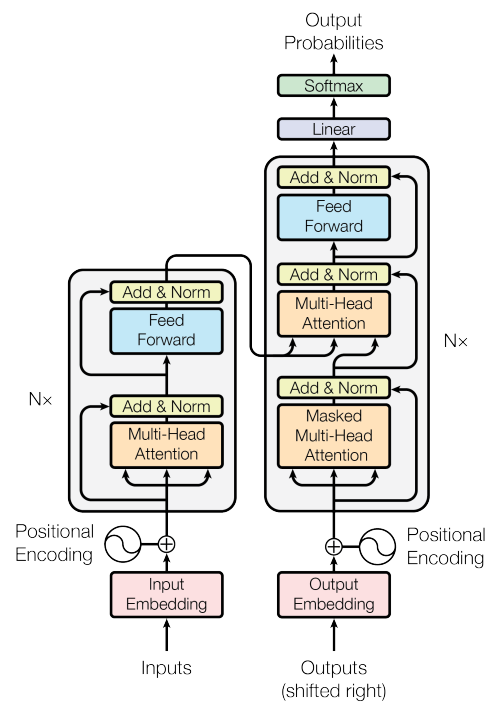
\includegraphics[scale=0.5]{assets/pics/transformer-achitecture.png}
\centering
\caption{Arsitektur model \emph{transformer}.\\\hspace{\textwidth}Referensi gambar: \citep{DBLP:journals/corr/VaswaniSPUJGKP17}}.
\end{figure}

\emph{Transformer} merupakan tipe arsitektur \emph{artificial neural networks} yang digunakan untuk memecahkan masalah transformasi dari urutan masukan (\emph{input}) menjadi urutan keluaran (\emph{output}) dalam suatu aplikasi \emph{deep learning} \citep{transformers-self-attention-to-the-rescue}. Keberadaan Transformer dianggap sebagai solusi dari permasalahan-permasalahan pada \emph{recurrent neural network} (RNN) dan \emph{long short-term memory} (LSTM), yang berkaitan dengan \emph{vanishing \& exploding gradient problem} pada RNN dan keterkaitan antar kata (\emph{relationship between words}) pada LSTM. Cara \emph{transformer} mengatasi masalah-masalah tersebut adalah dengan menggunakan \emph{self-attention}. \emph{Self-attention} merupakan mekanisme perhatian (\emph{attention}) yang menghubungkan posisi yang berbeda dari suatu urutan untuk menghitung representasi urutan tersebut \citep{DBLP:journals/corr/VaswaniSPUJGKP17}; sederhananya \emph{self-attention} merupakan mekanisme yang mempelajari keterkaitan antar kata (\emph{relationship between words}) yang gagal diatasi oleh LSTM. 

Kemudian, alasan mengapa \emph{transformer} dapat mengatasi \emph{vanishing \& exploding gradient problem}, adalah karena \emph{transformer} tidak bergantung pada perulangan (\emph{recurrent}) seperti yang dilakukan pada RNN, namun \emph{Transformer} bergantung kepada mekanisme perhatian (\emph{attention}) sepenuhnya, sehingga \emph{transformer} dapat terhindar dari perkalian angka-angka gradien kecil maupun besar yang dapat menyebabkan \emph{vanishing \& exploding gradient problem}. Kemudian, \emph{transformer} memungkinkan paralelisasi yang lebih signifikan dari arsitektur-arsitektur lainnya. Hal tersebut yang membuat \emph{transformer} menjadi \emph{state-of-the-art} model dari perkembangan arsitektur \emph{artificial neural networks} sampai saat ini.

%-----------------------------------------------------------------------------%
\section{\emph{Pre-trained Language Model}}
\label{2.5}
%-----------------------------------------------------------------------------%
Pada bagian ini, akan dipaparkan berbagai macam \emph{pre-trained language model} yang akan digunakan pada penelitian saat ini. Sederhananya, \emph{pre-trained language model} adalah model bahasa yang telah dilatih terlebih dahulu pada korpus teks yang besar untuk mempelajari pola bahasa dan representasi dari suatu kata. Proses \emph{training} model biasa dilakukan dengan teknik: belajar untuk memprediksi atau menghasilkan kata berikutnya dalam sebuah kalimat berdasarkan konteks kata sebelumnya dan/atau setelahnya (\emph{masked language modelling}) ataupun dengan memprediksi apakah suatu kalimat ada setelah kalimat lainnya (\emph{next sentence prediction}), hal tersebut bertujuan untuk menangkap pola statistik dan hubungan semantik dalam suatu bahasa. Proses ini memungkinkan model untuk mempelajari "\emph{word embeddings}" dan representasi kontekstual yang menyimpan informasi tentang makna kata, struktur sintaksis, dan beragam hal lainnya \citep{radford2018improving}.

%-----------------------------------------------------------------------------%
\subsection{BERT}
\label{2.5.1}
%-----------------------------------------------------------------------------%

BERT yang merupakan singkatan dari \emph{Bidirectional Encoder Representations from Transformers} merupakan salah satu \emph{pre-trained language model} yang dikembangkan oleh Google dan secara spesifik bertujuan sebagai representasi suatu bahasa atau dalam kata lain sebagai \emph{language representation models}. BERT sengaja dirancang untuk belajar representasi bahasa secara dua arah, yaitu: kiri ke kanan, dan kanan ke kiri. BERT dapat digunakan sebagai model untuk menjawab pertanyaan (\emph{question answering task}), inferensi bahasa, dan lain-lain \citep{devlin-etal-2019-bert}. Untuk jumlah komponen dalam model BERT itu sendiri, dapat dipaparkan sebagai berikut: untuk jenis BERT-\emph{base}, \emph{layer}-nya sebanyak 12 \emph{layer}, \emph{hidden-size} sebanyak 768, dan banyaknya \emph{self-attention heads} sebanyak 12, dan terakhir, banyaknya parameter sebanyak 110 juta parameter; kemudian untuk jenis BERT-\emph{large}, \emph{layer}-nya sebanyak 24 \emph{layer}, \emph{hidden-size} sebanyak 1024, dan banyaknya \emph{self-attention heads} sebanyak 16, dan terakhir, banyaknya parameter sebanyak 340 juta parameter. BERT sendiri secara orisinil dilatih dengan bahasa Inggris saja, namun, untuk kepentingan penelitian ini, kita menggunakan IndoBERT, yaitu BERT yang dilatih dengan bahasa Indonesia \citep{koto2020indolem}.

Arsitektur dari model BERT itu sendiri mengusung arsitektur \emph{multi-layer bidirectional Transformer encoder}, yaitu: model yang memiliki beberapa \emph{layer} dan bersifat dua arah (\emph{bidirectional}), hal tersebut berbeda dengan kebanyakan arsitektur model yang biasanya bersifat satu arah (\emph{directional}). Menurut 
\citet{devlin-etal-2019-bert} penggunaan sifat \emph{bidirectional} ini ditekankan untuk memahami pentingnya kontribusi sifat \emph{bidirectional} pada keberhasilan performa \emph{training} BERT itu sendiri, karena kelebihan yang dimiliki sifat \emph{bidirectional} dibandingkan dengan sifat \emph{directional} biasa. Karena, menurut \citet{devlin-etal-2019-bert} dengan sifat \emph{bidirectional} akan memungkinkan setiap kata untuk secara langsung untuk dapat melatih kata masing-masing secara independen, dan model dapat dengan mudah memprediksi kata target dalam suatu konteks.

%-----------------------------------------------------------------------------%
\subsection{RoBERTa}
\label{2.5.2}
%-----------------------------------------------------------------------------%
RoBERTa yang merupakan singkatan dari \emph{A Robustly Optimized BERT Pretraining Approach} adalah salah satu model yang merupakan suatu \emph{pre-trained language model} pengembangan dari \emph{pre-trained language model} BERT. Modifikasi yang dilakukan oleh \citet{liu2019roberta} pada model BERT antara lain: memperbanyak waktu \emph{training} dengan jumlah \emph{batch} yang lebih besar, menghapus objektif \emph{next-sentence-prediction}, melatih model untuk \emph{sequence} yang lebih panjang, mengubah secara dinamis \emph{masking pattern} pada data latih, dan dilatih dengan \emph{dataset} baru yang lebih besar. 

Alasan mengapa dilakukan modifikasi tersebut adalah karena menurut \citet{liu2019roberta} setelah dilakukan evaluasi terhadap model BERT termasuk \emph{hyperparameters tuning} dan \emph{training set size}, model BERT dianggap \emph{ significantly undertrained} yang menyebabkan hasil performa dari BERT masih dirasa kurang baik oleh \citeauthor{liu2019roberta}. Oleh karena itu \citet{liu2019roberta} mengusulkan resep yang terbukti lebih baik untuk melatih model BERT, yaitu: RoBERTa; yang performanya dianggap setara atau melebihi kinerja semua metode pasca kemunculan model BERT.

%-----------------------------------------------------------------------------%
\subsection{XLM-RoBERTa}
\label{2.5.3}
%-----------------------------------------------------------------------------%
XLM-RoBERTa yang merupakan singkatan dari \emph{Cross-lingual Language Model For Robustly Optimized BERT Pretraining Approach} adalah salah satu \emph{pre-trained language model} yang merupakan suatu model pengembangan dari \emph{pre-trained language model} RoBERTa. Modifikasi yang dilakukan oleh \citet{conneau2020unsupervised} pada model RoBERTa adalah penggunaan banyak bahasa pada data latih model XLM-RoBERTa, yang mencakup sekitar 100 bahasa yang disadur dari halaman Wikipedia dengan beragam bahasa yang tersedia. Penggunaan banyak bahasa ini dipengaruhi oleh adanya model mBERT yang menggunakan data latih dari 104 bahasa.

Alasan mengapa dilakukan modifikasi tersebut adalah untuk menguji \emph{cross-lingual language understanding (XLU) task} untuk  memperoleh performa terbaik dalam \emph{task-task} lintas bahasa, seperti: \emph{cross-lingual classification, cross-lingual sequence labeling} dan \emph{cross-lingual question answering}. Karena kebutuhan model untuk \emph{task} lintas bahasa masih banyak dibutuhkan. Apalagi dengan anggapan bahwa dengan \emph{task} lintas bahasa dapat meningkatkan kinerja pada \emph{task} NLP lainnya dengan memanfaatkan struktur linguistik pada beragam bahasa tersebut.

%-----------------------------------------------------------------------------%
\section{\emph{Intermediate-Task Transfer Learning}}
\label{2.6}
%-----------------------------------------------------------------------------%

\begin{figure}[h]
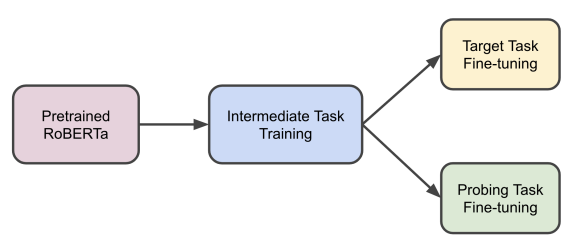
\includegraphics[width=\linewidth]{assets/pics/ittl-pipeline.png}
\centering
\caption{Salah satu contoh alur penggunaan \emph{Intermediate-Task Transfer Learning}.\\\hspace{\textwidth}Referensi gambar: \citep{pruksachatkun-etal-2020-intermediate}.}
\end{figure}

\emph{Intermediate-Task Transfer Learning} merupakan teknik peningkatan performa dengan melakukan \emph{fine-tuning} dengan \emph{dataset} tugas lain (\emph{intermediate task}) pada model \emph{Transformer}, lalu model yang sudah dilakukan \emph{fine-tuning} tersebut akan dilakukan \emph{fine-tuning} kembali untuk tugas tujuannya (\emph{target task}) \citep{pruksachatkun-etal-2020-intermediate}. Harapannya, dengan logis, bila suatu model sudah dilatih pada tugas lain, model tersebut cenderung akan memberikan hasil yang baik bila model yang sudah dilatih tersebut dilatih kembali di tugas yang berbeda, namun masih dalam lingkup domain \emph{task} yang relevan. Teknik \emph{Intermediate-Task Transfer Learning} ini memanfaatkan kelebihan yang terdapat pada arsitektur \emph{Transformer} yang sudah dilatih pada \emph{dataset} yang sangat besar; seharusnya kinerja \emph{Transformer} dapat ditingkatkan dengan melatih model lebih lanjut pada tugas perantara (\emph{intermediate task}) yang memiliki data yang lebih kaya, beragam, dan berkualitas; sebelum melakukan penyempurnaan model pada tugas target (\emph{target task}) via \emph{transfer learning}. 

Namun, menurut \citet{pruksachatkun-etal-2020-intermediate}, masih belum mengetahui kapan dan bagaimana cara tugas perantara (\emph{intermediate task}) mempengaruhi dan bermanfaat bagi tugas target (\emph{target task}). Untuk mengetahui hal tersebut, studi \citet{pruksachatkun-etal-2020-intermediate} menemukan beberapa hal menarik, antara lain: \emph{intermediate task} membutuhkan inferensi tingkat tinggi (\emph{high-level inference}) dan kemampuan penalaran (\emph{reasoning abilities}) yang baik agar dapat bermanfaat bagi tugas targetnya, kemudian kinerja dari tugas target sangat berkorelasi dengan kemampuan inferensi tingkat yang lebih tinggi seperti pengelompokan penyebutan kata dalam teks yang mengacu pada entitas dunia nyata yang sama \citep{coference-resolution}. Contoh dari \emph{intermediate task} yang dapat membantu meningkatkan performa \emph{target task} dari eksperimen \citeauthor{pruksachatkun-etal-2020-intermediate} adalah MNLI dan \emph{commonsense-oriented tasks} seperti CommonsenseQA, HellaSWAG, dan CosmosQA yang terbukti dapat memberikan peningkatan performa yang signifikan kepada sebagian \emph{target task} yang sedang diuji.

%-----------------------------------------------------------------------------%
\section{\emph{Task Recasting}}
\label{2.7}
%-----------------------------------------------------------------------------%
\emph{Task recasting} merupakan teknik untuk mengubah bentuk \emph{dataset} (atau model), dari satu \emph{task} ke \emph{task} lainnya. \emph{Task recasting} biasanya digunakan untuk menurunkan (\emph{derive}) \emph{dataset task} untuk dapat digunakan pada \emph{task} lainnya, karena ada kecenderungan untuk mendapatkan \emph{dataset} yang lebih bagus dan lebih \emph{robust}, bila diturunkan dari \emph{dataset task} lain \citep{DBLP:journals/corr/abs-1809-02922}. Pada konteks penelitian ini, akan dilakukan \emph{task recasting} antar \emph{question answering task} dengan \emph{sequence classification task (natural language inference)} sebagai alternatif metode eksperimen yang nanti akan dilaksanakan.

Namun, penggunaan \emph{task recasting} tidak hanya sebatas menggunakan teknik ini saja (tanpa penambahan eksperimen apapun), melainkan dibutuhkan eksperimen tambahan untuk menyelesaikan eksperimen yang menggunakan \emph{task recasting} ini, pada konteks penelitian ini contohnya seperti: \emph{task recasting} dengan memanfaatkan IndoNLI sebagai verifikator.

%-----------------------------------------------------------------------------%
\section{Sistem Metrik Evaluasi}
\label{2.8}
%-----------------------------------------------------------------------------%
Pada bagian ini, akan dipaparkan dua metrik evaluasi utama yang akan digunakan pada penelitian saat ini.

%-----------------------------------------------------------------------------%
\subsection{Metrik \emph{Exact Match}}
\label{2.8.1}
%-----------------------------------------------------------------------------%

\begin{figure}[h]
\vspace{3pt}
\hrule
\vspace{3pt}

\textbf{Jawaban Prediksi}: Joanne Rowling\\
\textbf{Jawaban \emph{Gold Truth}}: Joanne Rowling\\
\textbf{Skor}: 1

\vspace{3pt}
\hrule
\vspace{3pt}

\textbf{Jawaban Prediksi}: \emph{The Wizarding World of Harry Potter di Island of Adventure Time}\\
\textbf{Jawaban \emph{Gold Truth}}: \emph{The Wizarding World of Harry Potter di Islands of Adventure}
\textbf{Skor}: 0\\

\vspace{3pt}
\hrule
\vspace{3pt}

\textbf{Jawaban Prediksi}: Gramedia Pustaka Utama\\
\textbf{Jawaban \emph{Gold Truth}}: Gramedia Pustaka Utama\\
\textbf{Skor}: 1

\vspace{5pt}
\hrule
\vspace{5pt}

\textbf{Jawaban Prediksi}: Severus Snape\\
\textbf{Jawaban \emph{Gold Truth}}: Hermione Granger\\
\textbf{Skor}: 0

\vspace{3pt}
\hrule
\vspace{3pt}

\textbf{Jawaban Prediksi}: The Scotsman\\
\textbf{Jawaban \emph{Gold Truth}}: The Scotsman\\
\textbf{Skor}: 1

\vspace{3pt}
\hrule
\vspace{3pt}

\textbf{Skor Akhir \emph{Exact Match}}: $\frac{1+0+1+0+1}{5}=0.6$

\centering
\caption{Contoh cara perhitungan skor akhir metrik \emph{exact match}.}
\end{figure}

Metrik \emph{exact match} pada suatu sistem tanya jawab mengukur persentase dari jawaban prediksi yang sama persis dengan jawaban \emph{ground truth}-nya \citep{rajpurkar-etal-2016-squad}. Saat melakukan evaluasi sistem tanya jawab, biasanya jawaban prediksi model akan dibandingkan dengan jawaban \emph{ground truth} yang didapatkan dari anotator manusia atau anotator ahli, bila jawaban prediksi model sistem tanya jawab sama persis hingga detail terkecil tanpa ada \emph{typo}, variasi, perbedaan format penulisan, dan kesalahan (\emph{error}) apapun, maka akan dihitung sebagai \emph{exact match}.

Contohnya, misal: suatu pertanyaan hanya memiliki satu jawaban \emph{ground truth} yaitu "Ir. Soekarno" (dengan titik), maka metrik evaluasi \emph{exact match} menilai benar, bila jawaban prediksi model menghasilkan jawaban yang sama persis: "Ir. Soekarno", bila jawaban prediksi model menghasilkan "Ir Soekarno" atau "Ir. Sukarno", maka metrik metrik evaluasi \emph{exact match} akan menilai salah. Padahal, maknanya sama namun dengan penyertaan informasi tambahan atau jawaban prediksi memiliki format yang berbeda dari jawaban \emph{ground truth}, namun tetap dinilai salah oleh metrik evaluasi \emph{exact match}. Dengan hal tersebut, metrik evaluasi \emph{exact match} ini biasa digunakan sebagai tolak ukur bagi suatu sistem tanya jawab yang memberikan pengukuran kebenaran yang biner, yang menunjukkan apakah jawaban prediksi sama persis dengan jawaban yang diharapkan atau tidak.

%-----------------------------------------------------------------------------%
\subsection{Metrik Skor F1}
\label{2.8.2}
%-----------------------------------------------------------------------------%

\begin{figure}[h]
\vspace{3pt}
\hrule
\vspace{3pt}

\textbf{Jawaban Prediksi}: Joanne Rowling\\
\textbf{Jawaban \emph{Gold Truth}}: Joanne Rowling\\
\textbf{\emph{Precision}}: $\frac{2}{2}=1$\\
\textbf{\emph{Recall}}: $\frac{2}{2}=1$\\
\textbf{Skor F1}: $\frac{2 \times 1 \times 1}{1 + 1}=1$

\vspace{3pt}
\hrule
\vspace{3pt}

\textbf{Jawaban Prediksi}: \emph{The Wizarding World of Harry Potter di Island of Adventure Time}\\
\textbf{Jawaban \emph{Gold Truth}}: \emph{The Wizarding World of Harry Potter di Islands of Adventure}\\
\textbf{\emph{Precision}}: $\frac{9}{11}=0.818$\\
\textbf{\emph{Recall}}: $\frac{9}{10}=0.9$\\
\textbf{Skor F1}: $\frac{2 \times 0.82 \times 0.9}{0.82 + 0.9}=0.857$

\vspace{3pt}
\hrule
\vspace{3pt}

\textbf{Jawaban Prediksi}: Gramedia Pustaka Utama\\
\textbf{Jawaban \emph{Gold Truth}}: Gramedia Pustaka Utama\\
\textbf{\emph{Precision}}: $\frac{2}{2}=1$\\
\textbf{\emph{Recall}}: $\frac{2}{2}=1$\\
\textbf{Skor F1}: $\frac{2 \times 1 \times 1}{1 + 1}=1$

\vspace{5pt}
\hrule
\vspace{5pt}

\textbf{Jawaban Prediksi}: Severus Snape\\
\textbf{Jawaban \emph{Gold Truth}}: Hermione Granger\\
\textbf{\emph{Precision}}: $\frac{0}{2}=0$\\
\textbf{\emph{Recall}}: $\frac{0}{2}=0$\\
\textbf{Skor F1}: $\frac{2 \times 0 \times 0}{0 + 0}=1$

\vspace{3pt}
\hrule
\vspace{3pt}

\textbf{Jawaban Prediksi}: The Scotsman\\
\textbf{Jawaban \emph{Gold Truth}}: The Scotsman\\
\textbf{\emph{Precision}}: $\frac{2}{2}=1$\\
\textbf{\emph{Recall}}: $\frac{2}{2}=1$\\
\textbf{Skor F1}: $\frac{2 \times 1 \times 1}{1 + 1}=1$

\vspace{3pt}
\hrule
\vspace{3pt}

\textbf{Skor Akhir \emph{F1}}: $\frac{1+0.857+1+0+1}{5}=0.771$

\centering
\caption{Contoh cara perhitungan skor akhir metrik F1.}
\end{figure}

Metrik skor F1  pada suatu sistem tanya jawab mengukur rata-rata tumpang-tindih (\emph{average overlap}) antara jawaban prediksi dan jawaban \emph{ground truth} \citep{rajpurkar-etal-2016-squad}. Berbeda dengan skor F1 pada umumnya, bagi \citeauthor{rajpurkar-etal-2016-squad} skor F1 pada sistem tanya jawab, jawaban prediksi dan jawaban \emph{ground truth} diperlakukan sebagai kumpulan token (\emph{bag of token}), Skor F1 sejatinya juga mengukur bagaimana performa dari suatu sistem tanya jawab dengan memperhatikan nilai \emph{precision} dan \emph{recall}-nya masing-masing. 


\begin{equation}
Precision = \frac{True \; Positive}{True \; Positive + False \; Positive}
\end{equation}

Nilai \emph{precision} dapat dimaknai dengan: seberapa baik prediksi model memilih jawaban yang benar dan terprediksi benar dibandingkan dengan semua jawaban yang terprediksi benar. Biasanya nilai \emph{precision} ini bertujuan untuk mengukur kesalahan pada kasus-kasus terprediksi positif. Namun, nilai \emph{precision} tidak melibatkan kasus-kasus yang terprediksi negatif, dimana hal ini bisa menjadi celah untuk yang dapat berkembang menjadi buruknya hasil prediksi negatif dari suatu sistem tanya jawab.

\begin{equation}
Recall = \frac{True \; Positive}{True \; Positive + True \; Negative}
\end{equation}

Kemudian, nilai \emph{recall} dapat dimaknai dengan: seberapa baik prediksi model memilih jawaban yang benar dan terprediksi benar dibandingkan dengan semua jawaban yang \emph{ground truth}-nya benar. Biasanya nilai \emph{recall} ini bertujuan untuk mengukur kesalahan pada kasus-kasus terprediksi negatif. Hal tersebut merupakan solusi dari permasalahan \emph{precision} sebelumnya, dimana nilai \emph{recall} juga mempertimbangkan kasus yang terprediksi negatif. Namun, disini terbalik dengan permasalahan \emph{precision}, nilai \emph{recall} tidak melibatkan kasus-kasus yang terprediksi positif, dimana hal ini bisa menjadi celah untuk yang dapat berkembang menjadi buruknya hasil prediksi positif dari suatu sistem tanya jawab.

\begin{equation}
F1 \; Score = \frac{2 \times Precision \times Recall}{Precision + Recall}
\end{equation}

Logikanya, bila hasil metrik \emph{precision} mencapai 100\% maka hasil metrik \emph{recall} sama dengan 0\%, sebaliknya bila hasil metrik \emph{recall} mencapai 100\% maka hasil metrik \emph{precision} sama dengan 0\%. Maka dari itu, hadir metrik skor F1 yang merupakan \emph{harmonic mean} dari metrik \emph{precision} dan metrik \emph{recall}, dimana skor F1 berusaha mengukur seberapa baik metrik \emph{precision} sekaligus metrik \emph{recall} dalam suatu prediksi. Sederhananya, skor F1 adalah metrik perbandingan seimbang (\emph{balanced comparison}) dari hasil representasi nilai tunggal (\emph{single value}) dari metrik \emph{precision} sekaligus metrik \emph{recall}. Dengan hal tersebut, metrik evaluasi skor F1 ini biasa digunakan sebagai tolak ukur bagi suatu sistem tanya jawab yang memberikan pengukuran kebenaran dengan memperhatikan metrik \emph{precision} dan metrik \emph{recall} secara bersamaan, yang menunjukkan seberapa mirip jawaban prediksi dengan jawaban yang diharapkan atau tidak, hal tersebut sekaligus dapat menghitung performa prediksi jawaban dengan lebih toleran dengan tanpa terlalu memperhatikan detail terkecil, seperti: \emph{typo}, variasi, perbedaan format penulisan, dan kesalahan (\emph{error}) kecil yang padahal memiliki makna yang sama dengan jawaban \emph{ground truth}-nya.
\clearchapter
%-----------------------------------------------------------------------------%
\chapter{\babTiga}
%-----------------------------------------------------------------------------%
Bab ketiga ini menjelaskan tentang rancangan dan metodologi yang penulis lakukan dalam penelitian ini. Sub-bab 3.1 menjelaskan mengenai tahapan penelitian yang akan penulis lakukan. Sub-bab 3.2 menjelaskan bagaimana persiapan data, model, dan metode yang akan dilakukan pada penelitian ini. Sub-bab 3.3 menjelaskan pelatihan model dan alur eksperimen yang dilakukan. Sub-bab 3.4 lalu menjelaskan metrik umum yang digunakan setiap metode dan metrik khusus yang digunakan untuk setiap metode.

%-----------------------------------------------------------------------------%
\section{Tahapan Penelitian}
%-----------------------------------------------------------------------------%
Pada sub-bab ini, akan dijelaskan mengenai tahapan penelitian yang penulis gunakan pada penelitian ini. Tahapan penelitian yang penulis lakukan adalah sebagai berikut:

\begin{itemize}
    
    \item \textbf{Persiapan data, model, dan metode}: Pada tahap ini penulis melakukan pencarian untuk memilih data, model, dan metode eksperimen apa saja yang akan digunakan dalam penelitian ini. Tahap ini meliputi pemilihan data dan model yang akan digunakan untuk tiap metode dan penjelasan metode yang dipakai untuk penelitian. Pada akhirnya, penulis menentukan beberapa \emph{dataset} sistem tanya jawab: SQuAD-ID, TyDi-QA-ID, dan IDK-MRC sebagai dataset pengujian sistem tanya jawab, dan pada penelitian ini menggunakan model-model seperti: \emph{indolem/indobert-base-uncased, indobenchmark/indobert-large-p2, xlm-roberta-base}, dan \emph{xlm-roberta-large}. Kemudian, untuk metode penelitian, penulis memutuskan untuk menggunakan tiga metode eksperimen, yaitu: \emph{intermediate-task transfer learning}, \emph{task recasting} dengan IndoNLI sebagai verifikator, dan \emph{task recasting} dengan IndoNLI sebagai penghasil jawaban. Hasil dari tahap ini adalah data yang akan digunakan pada tahap selanjutnya.

    \item \textbf{Eksplorasi \emph{dataset} (EDA)}: Pada tahap ini penulis melakukan eksplorasi dari \emph{dataset} sistem tanya jawab yang telah dipilih, yaitu: SQuAD-ID, TyDi-QA-ID, dan IDK-MRC. Eksplorasi \emph{dataset} (EDA) dilakukan dengan bertujuan untuk mengerti karakteristik dari suatu \emph{dataset} sistem tanya jawab yang sedang diproses.
    
    \item \textbf{Pelatihan model dan eksperimen}: Pada tahap ini penulis melakukan pelatihan model dan eksperimen-eksperimen berdasarkan data, model, dan metode yang sudah dipilih pada tahap sebelumnya. Tahap ini meliputi pelatihan model yang akan digunakan untuk tiap metode. Hasil dari tahap ini adalah model yang sudah dilatih berdasarkan metode yang telah dipilih yang menghasilkan hasil eksperimen untuk dilakukan analisis pada tahap berikutnya.

    \item \textbf{Evaluasi dan analisis hasil}: Pada tahap ini penulis melakukan evaluasi dan analisis berdasarkan hasil yang sudah didapatkan pada tahap sebelumnya. Tahap ini meliputi pemilihan metrik evaluasi yang digunakan untuk setiap metode eksperimen penelitian.

\end{itemize}

%-----------------------------------------------------------------------------%
\section{Persiapan Data, Model, dan Metode}
%-----------------------------------------------------------------------------%
Pada sub-bab ini, akan dijelaskan mengenai data, model, dan metode yang penulis gunakan pada eksperimen-eksperimen pada penelitian ini. 

%-----------------------------------------------------------------------------%
\subsection{Data dan Model}
%-----------------------------------------------------------------------------%
Data yang penulis gunakan dapat terbagi menjadi dua bagian, data NLI dan data sistem tanya jawab. Untuk data NLI, penulis hanya menggunakan satu \emph{dataset}, yaitu: \emph{dataset} IndoNLI \citep{mahendra-etal-2021-indonli}. Alasan menggunakan \emph{dataset} ini adalah: karena topik utama penelitian ini adalah melanjutkan topik penelitian \citet{mahendra-etal-2021-indonli} terkait pemanfaatan \emph{dataset} IndoNLI pada beragam tugas (\emph{task}) bidang NLP, salah satunya adalah sistem tanya jawab (\emph{question answering}). Kemudian, untuk data sistem tanya jawab, penulis menggunakan tiga \emph{dataset} sebagai tolak ukur (\emph{benchmark}) dari evaluasi sistem tanya jawab yang penulis rancang, yaitu: \emph{dataset} SQuAD-ID \citep{muis2020sequencetosequence}, TyDi-QA-ID \citep{cahyawijaya-etal-2021-indonlg}, IDK-MRC \citep{putri-oh-2022-idk}. Alasan menggunakan ketiga \emph{dataset} ini adalah: karena menurut penulis, ketiga \emph{dataset} ini merupakan \emph{dataset} terbaik untuk dijadikan tolak ukur (\emph{benchmark}) sistem tanya jawab berbahasa Indonesia. Penggunaan tiga \emph{dataset} sekaligus juga penulis tujukan agar sistem tanya jawab dapat menangkap pola-pola variasi beragam \emph{dataset} sistem tanya jawab, sehingga sistem tanya jawab buatan penulis berhasil menggeneralisasikan pola-pola tersebut untuk menghasilkan prediksi jawaban yang lebih \emph{robust}.

%-----------------------------------------------------------------------------%
\subsection{Metode Eksperimen}
%-----------------------------------------------------------------------------%
Pada sub-bab ini, akan dijelaskan beberapa metode yang penulis pilih, yaitu: \emph{intermediate-task transfer learning}, \emph{task recasting} dengan IndoNLI sebagai verifikator jawaban, dan \emph{task recasting} dengan IndoNLI sebagai penghasil jawaban. 

%-----------------------------------------------------------------------------%
\subsubsection{\emph{Intermediate-Task Transfer Learning}}
%-----------------------------------------------------------------------------%
Pada tahapan eksperimen ini, penulis menggunakan metode yang persis digunakan oleh \citep{pruksachatkun-etal-2020-intermediate}, yaitu dengan memecah tugasnya menjadi dua, yaitu: \emph{intermediate task} dan \emph{target task}. Pada penelitian ini, \emph{intermediate task} yang dipilih adalah \emph{sequence classification task} dengan menggunakan \emph{dataset} IndoNLI, dan \emph{target task} yang dipilih adalah \emph{question answering task} dengan menggunakan \emph{dataset} SQuAD-ID, TyDi-QA-ID, dan IDK-MRC. Untuk alur eksperimen tahap ini, akan dijelaskan pada sub-bab selanjutnya.

%-----------------------------------------------------------------------------%
\subsubsection{\emph{Task Recasting} dengan IndoNLI sebagai verifikator}
%-----------------------------------------------------------------------------%
Pada tahapan eksperimen ini, penulis menggunakan metode yang persis digunakan oleh \citep{chen-etal-2021-nli-models}, yaitu dengan melakukan penyaringan (\emph{filtering}) prediksi jawaban dengan parameter hasil label NLI-nya. Pada penelitian ini, prediksi jawaban oleh model \emph{question answering} tidak diganggu sama sekali, setelah prediksi jawaban didapatkan, baru dilakukan penyaringan (\emph{filtering}) prediksi jawabannya. Untuk alur eksperimen tahap ini, akan dijelaskan pada sub-bab selanjutnya. 

%-----------------------------------------------------------------------------%
\subsubsection{\emph{Task Recasting} dengan IndoNLI sebagai penghasil jawaban}
%-----------------------------------------------------------------------------%
\todo

%-----------------------------------------------------------------------------%
\section{Eksplorasi \emph{dataset} (EDA)}
%-----------------------------------------------------------------------------%
Pada sub-bab ini, akan dijelaskan mengenai eksplorasi \emph{dataset} (EDA) sistem tanya jawab yang telah dipilih sebelumnya. Eksplorasi yang penulis lakukan sama persis dengan apa yang telah dilakukan \citet{nguyen-etal-2020-vietnamese} dan \citet{rajpurkar-etal-2016-squad} pada tahapan ekplorasi \emph{dataset machine reading comprehension} untuk bahasa Vietnam. Ada beberapa bagian yang penulis jadikan bahan eksplorasi, antara lain:

\begin{itemize}

    \item \emph{Overview Statistics}

        \begin{itemize}
            \item Banyaknya artikel.
            \item Banyaknya konteks.
            \item Banyaknya pertanyaan.
            \item Banyaknya jawaban yang eksis.
            \item Banyaknya jawaban yang tidak eksis.
            \item Rata-rata panjang kata dari konteks.
            \item Rata-rata panjang kata dari pertanyaan.
            \item Rata-rata panjang kata dari jawaban.
            \item \emph{Vocabulary size}.
        \end{itemize}

    \item \emph{Length-based analysis}

        \begin{itemize}
            \item Rincian distribusi panjang kata dari konteks.
            \item Rincian distribusi panjang kata dari pertanyaan.
            \item Rincian distribusi panjang kata dari jawaban.
        \end{itemize}
        
    \item \emph{Type-based analysis}

        \begin{itemize}
            \item \emph{Question type}.
            \item \emph{Reasoning type}.
            \item \emph{Answer type}.
        \end{itemize}

\end{itemize}

Properti-properti di atas yang akan menjadi bahan evaluasi dan analisis penelitian ini yang telah tertuang pada \hyperref[sec:rumusanMasalah]{rumusan masalah} dan \hyperref[sec:tujuanPenelitian]{tujuan penelitian} yang telah dituliskan di \hyperref[bab:1]{bab 1} di atas. Penggunaan properti-properti di atas ditujukan untuk mendalami dan menambah wawasan terkait \emph{dataset} sistem tanya jawab.


%-----------------------------------------------------------------------------%
\section{Pelatihan Model dan Eksperimen}
%-----------------------------------------------------------------------------%
Pada sub-bab ini, akan dijelaskan mengenai pelatihan model dan eksperimen yang penulis lakukan pada pada penelitian ini. 

%-----------------------------------------------------------------------------%
\subsection{\emph{Intermediate-Task Transfer Learning}}
%-----------------------------------------------------------------------------%
Alur penelitian tahapan \emph{intermediate-task transfer learning} yang penulis lakukan adalah sebagai berikut:

\begin{itemize}
    
    \item Tiga model yang sudah dipilih pada tahapan persiapan data, model, dan metode sebelumnya akan diunduh via platform Hugging Face untuk mengambil \emph{tokenizer} dan model \emph{baseline}-nya.

    \item Model-model tersebut dilatih dalam \emph{sequence classification task} dengan menggunakan \emph{dataset} IndoNLI untuk dapat menentukan hubungan suatu premis dan hipotesis, apakah hubungan \emph{entailment, contradiction}, atau \emph{neutral}. Pada tahap ini, \emph{sequence classification task} disebut sebagai \emph{intermediate task}.

    \item Setelah dilatih, bobot-bobot hasil latihan \emph{sequence classification task} tersebut dipindahkan ke model khusus sistem tanya jawab (\emph{question answering task}), yang basisnya sama dengan tiga model yang sudah dipilih pada tahapan persiapan data, model, dan metode sebelumnya.

    \item Model \emph{question answering task} tersebut dilatih ulang dengan menggunakan bobot dari \emph{sequence classification task} sebelumnya dan menggunakan tiga \emph{dataset} sistem tanya jawab yang sebelumnya dipilih, yaitu: SQuAD-ID, TyDi-QA-ID, dan IDK-MRC. Pada tahap ini, kita bisa memilih \emph{layer} apa saja yang akan dilatih ulang, apakah semua \emph{layer} atau hanya \emph{layer} teratas (\emph{classifier}) saja yang akan dilatih ulang, eksperimen dengan hanya \emph{layer} teratas yang akan dilatih ulang dapat disebut juga \emph{freezing layer} \citep{lee2019elsa}. Pada tahap ini, \emph{question answering task} disebut sebagai \emph{target task}.

    \item Terakhir, menyimpan keseluruhan hasil eksperimen untuk dilakukan evaluasi dan analisis hasil eksperimen.

\end{itemize}

%-----------------------------------------------------------------------------%
\subsection{\emph{Task Recasting} dengan IndoNLI sebagai verifikator}
%-----------------------------------------------------------------------------%
Alur penelitian tahapan task Recasting dengan IndoNLI sebagai verifikator yang penulis lakukan adalah sebagai berikut:

\begin{itemize}
    
    \item Tiga model yang sudah dipilih pada tahapan persiapan data, model, dan metode sebelumnya akan diunduh via platform Hugging Face untuk mengambil \emph{tokenizer} dan model \emph{baseline}-nya. Model-model ini langsung diubah ke \emph{question answering task}.
    
    \item Model-model tersebut dilatih dalam \emph{question answering task} dengan menggunakan tiga \emph{dataset} sistem tanya jawab, yaitu: SQuAD-ID, TyDi-QA-ID, dan IDK-MRC untuk dapat memprediksi jawaban dari konteks yang telah diberikan.
    
    \item Setelah dilatih, model-model tersebut memprediksi jawaban dari konteks (dari \emph{test set}) yang sudah tersedia.
    
    \item Kemudian, pada tahap ini dilakukan perubahan struktur hasil prediksi sistem tanya jawab menjadi struktur yang dapat dinilai berdasarkan parameter label NLI-nya, pengubahan ini dapat dilakukan dengan \emph{smoothing}. \emph{Smoothing} sendiri merupakan istilah yang digunakan untuk menyebutkan pengubahan dari pasangan jawaban dan pertanyaan menjadi hipotesis deklaratif dalam sudut pandang NLI. Selanjutnya, terdapat berbagai parameter, meliputi:
    
    \begin{itemize}
        
        \item Tipe \emph{filtering}: pada tahap ini, penulis dapat memilih label NLI apa saja yang masih bisa diterima sebagai jawaban, pilihannya ada dua, yaitu: hanya label \emph{entailment}; atau label \emph{entailment} atau label \emph{neutral}.
        
        \item Tipe \emph{smoothing}: pada tahap ini, penulis dapat memilih teknik \emph{smoothing}. Tipe smoothing dapat dipilih dari berbagai pilihan, seperti: \emph{rule-based, paraphraser machine learning}, dan lain-lain.
        
        \item Pencarian iterasi maksimum: pada tahap ini, penulis dapat memilih berapa kali iterasi pencarian jawaban yang sesuai dengan parameter label NLI.
        
    \end{itemize}
    
    \item Kemudian, dilakukan penyaringan (\emph{filtering}) jawaban, alurnya dilakukan sebagai berikut:
    
    \begin{itemize}
        
        \item Jika label hasil prediksi jawaban dari model \emph{question answering task} sudah sesuai dengan label hasil pilihan tipe \emph{filtering} di atas, maka hasil jawaban tersebut disimpan dan dikeluarkan sebagai prediksi final.
        
        \item Sedangkan, jika label hasil prediksi jawaban dari model \emph{question answering task} belum sesuai dengan label hasil pilihan tipe \emph{filtering} di atas, maka akan dilakukan pencarian berdasarkan hasil pilihan parameter pencarian iterasi maksimum di atas. Pencarian ini didasari dengan ide \emph{arg max} pada \emph{tensor} hasil prediksi, sehingga mencari \emph{arg max} kedua, \emph{arg max} ketiga, dan \emph{arg max} seterusnya, sesuai dengan pilihan parameter pencarian iterasi maksimum yang sudah dipilih di atas. Setiap iterasi pencarian ini, akan disimpan jawaban dan label NLI-nya. Bila sudah menemukan label dan jawaban yang sesuai dengan label hasil pilihan tipe \emph{filtering} di atas, maka hasil jawaban tersebut disimpan dan dikeluarkan sebagai prediksi final.
        
        \item Bila sampai iterasi terakhir tidak ditemukan juga hasil prediksi jawaban yang sesuai dengan label hasil pilihan tipe \emph{filtering} di atas, maka akan otomatis menyimpan jawaban kosong sebagai prediksi final. Hal ini ditujukan untuk mencakup \emph{unanswerable question} yang terdapat pada tiga \emph{dataset} pilihan sistem tanya jawab penelitian ini.
        
    \end{itemize}
    
    \item Terakhir, menyimpan keseluruhan hasil eksperimen untuk dilakukan evaluasi dan analisis hasil eksperimen.

\end{itemize}

%-----------------------------------------------------------------------------%
\subsection{\emph{Task Recasting} dengan IndoNLI sebagai penghasil jawaban}
%-----------------------------------------------------------------------------%
\todo

%-----------------------------------------------------------------------------%
\section{Evaluasi dan Analisis Hasil}
%-----------------------------------------------------------------------------%
Pada sub-bab ini, akan dilakukan tahapan evaluasi dan analisis hasil ketiga metode itu dengan \emph{baseline} tanpa melakukan eksperimen sama sekali, kemudian, metrik yang dipilih sebagai bahan evaluasi dan analisis secara umum ada dua, yaitu: \emph{exact match} (atau bisa direpresentasikan sebagai akurasi) dan skor F1 berdasarkan \emph{token} prediksi jawaban. Pemilihan kedua metrik evaluasi tersebut didasari oleh keinginan penulis untuk mencontoh \citep{rajpurkar-etal-2016-squad} dalam penggunaan metrik evaluasi sistem tanya jawab. Namun, secara khusus, metrik evaluasi yang digunakan oleh setiap metode akan berbeda, contohnya akan dijelaskan pada sub-bab selanjutnya.

%-----------------------------------------------------------------------------%
\subsection{\emph{Intermediate-Task Transfer Learning}}
%-----------------------------------------------------------------------------%
Metrik yang penulis gunakan pada tahap ini adalah: \emph{exact match} dan skor F1 berdasarkan \emph{token} prediksi jawaban saja (sama persis dengan evaluasi \citep{rajpurkar-etal-2016-squad}). Analisis dan evaluasi hanya akan didasari oleh kedua metrik tersebut. Hal tersebut penulis contoh dari \citet{rajpurkar-etal-2016-squad}, untuk dapat membandingkan hasil sebelum dilakukan \emph{intermediate-task transfer learning} dan setelah dilakukan \emph{intermediate-task transfer learning}. Dengan kedua metrik tersebut, seharusnya sudah dapat terbaca penurunan ataupun peningkatan dari model sistem tanya jawab yang telah dirancang.

%-----------------------------------------------------------------------------%
\subsection{\emph{Task Recasting} dengan IndoNLI sebagai verifikator}
%-----------------------------------------------------------------------------%
Metrik yang penulis gunakan pada tahap ini adalah: \emph{exact match} berdasarkan \emph{token prediksi} jawaban, skor F1 berdasarkan \emph{token} prediksi jawaban, akurasi berdasarkan parameter label NLI, dan skor F1 berdasarkan parameter label NLI. Analisis dan evaluasi akan didasari oleh keempat metrik tersebut. Hal tersebut bertujuan untuk mengetahui penurunan atau peningkatan hasil prediksi jawaban yang tersaring (\emph{filtered}). Dengan keempat metrik tersebut, seharusnya sudah dapat terbaca bagaimana kualitas sistem penyaringan (\emph{filtering}) sistem tanya jawab kita, apakah jawaban benar tidak masuk prediksi final karena terhalang oleh label NLI, ataupun sebaliknya, apakah jawaban salah justru masuk prediksi final karena label NLI-nya sudah sesuai.

%-----------------------------------------------------------------------------%
\subsection{\emph{Task Recasting} dengan IndoNLI sebagai penghasil jawaban}
%-----------------------------------------------------------------------------%
\todo
\clearchapter
%-----------------------------------------------------------------------------%
\chapter{\babEmpat}
\label{bab:4}
%-----------------------------------------------------------------------------%
Bab keempat ini menjelaskan tentang implementasi teknis yang penulis lakukan dalam penelitian ini. Sub-bab 4.1 menjelaskan mengenai \emph{training} \emph{sequence classification task}. Sub-bab 4.2 menjelaskan mengenai  \emph{training} \emph{baseline} model \emph{question answering task}. Sub-bab 4.3 menjelaskan mengenai metode \emph{intermediate-task transfer learning}. Sub-bab 4.4 lalu menjelaskan mengenai metode \emph{task recasting} dengan IndoNLI sebagai verifikator.

%-----------------------------------------------------------------------------%
\section{\emph{Training} \emph{Sequence Classification Task}}
%-----------------------------------------------------------------------------%
Pada sub-bab ini, akan dijelaskan mengenai \emph{training} model pada tugas \emph{sequence classification} dalam belajar \emph{natural language inference} yang penulis lakukan pada pada penelitian ini. 

%-----------------------------------------------------------------------------%
\subsection{Pengambilan Parameter Untuk \emph{Training Sequence Classification Task}}
%-----------------------------------------------------------------------------%
Pengambilan parameter untuk \emph{training sequence classification task} menggunakan bantuan \emph{library} dari \texttt{argparse}. Penulis gunakan \texttt{argparse} agar dapat menjalankan eksperimen via \emph{terminal} bukan dengan satu-satu menjalankan via \emph{notebook}. Parameter yang dapat digunakan dalam \emph{training sequence classification task} ini meliputi: nama model, nama \emph{dataset}, jumlah \emph{epoch}, jumlah sampel data, jumlah \emph{learn rate}, jumlah \emph{seed}, jumlah \emph{batch size}, jumlah \emph{gradient accumulation}, dan token akun Hugging Face agar dapat otomatis \emph{push} ke akun Hugging Face-nya. Untuk pilihan nilai dari masing-masing parameternya, penulis sertakan di tabel bawah ini.

\begin{table}[h!]
\centering
\begin{tabular}{|P{2.0in}|P{4.0in}|}
 \hline
 Parameter & Pilihan Nilai \\ [0.5ex] 
 \hline
 Nama model & \texttt{indobert-base-uncased}, \texttt{indobert-large-p2}, \texttt{xlm-roberta-large} \\ 
 Nama data & IndoNLI-\emph{basic}, IndoNLI-\emph{translated}, IndoNLI-\emph{augmented} \\
 Jumlah \emph{epoch} & Isi dengan \emph{integer} berapapun \\
 Jumlah sampel & Isi dengan \emph{integer} berapapun, atau dengan \emph{string} \texttt{max} \\
 Jumlah \emph{learn rate} & Isi dengan \emph{float} berapapun \\ 
 Jumlah \emph{seed} & Isi dengan \emph{integer} berapapun \\ 
 Jumlah \emph{batch size} & Isi dengan \emph{integer} berapapun \\ 
 Jumlah \emph{gradient accumulation} & Isi dengan \emph{integer} berapapun \\ 
 \emph{Token} & Isi dengan \emph{string} \emph{token} yang tertera pada Hugging Face \\[1ex] 
 \hline
\end{tabular}
\caption{Tabel parameter dan pilihan nilai pada \emph{training sequence classification} IndoNLI}
\end{table}

%-----------------------------------------------------------------------------%
\subsection{Pemilihan \emph{Hyperparameter} Untuk \emph{Sequence Classification Task}}
%-----------------------------------------------------------------------------%
Selain dari \emph{hyperparameter} yang dapat diatur pada pengambilan parameter sebelumnya, terdapat beberapa \emph{hyperparameter} permanen untuk penelitian ini, berikut \emph{hyperparameter} yang tidak bisa diubah-ubah via \texttt{argparse}.

\begin{table}[h]
\centering
\begin{tabular}{||c | c||} 
 \hline\hline
 \emph{Hyperparameter} & Nilai \\ [0.5ex] 
 \hline\hline
 MAX LENGTH & 512 \\ 
 STRIDE & 128 \\
 LOGGING STEPS & 50 \\
 WARMUP RATIO & 0.0 \\
 WEIGHT DECAY & 0.0 \\ 
 EVAL STEPS RATIO & 0.5 \\ [1ex] 
 \hline\hline
\end{tabular}
\caption{Tabel \emph{hyperparameter} pada \emph{training sequence classification} IndoNLI}
\end{table}

%-----------------------------------------------------------------------------%
\subsection{Mengimpor \emph{Dataset} IndoNLI}
%-----------------------------------------------------------------------------%
Pada tahap ini, akan dijalankan pengambilan \emph{dataset} IndoNLI dari Hugging Face maupun GitHub dan penyamaan format \texttt{DatasetDict}. Tujuan dilakukan hal tersebut agar dapat lebih mempermudah eksperimen kedepannya. Untuk \emph{dataset} IndoNLI-\emph{basic}, penulis hanya mengambil via Hugging Face saja dengan fungsi \texttt{load\char`_dataset("indonli")}. 

Lalu, untuk \emph{dataset} IndoNLI-\emph{translated}, penulis mengambil via pranala: \href{https://huggingface.co/datasets/muhammadravi251001/translated-indo-nli}{\texttt{huggingface.co/datasets/muhammadravi251001/translated-indo-nli}} dan melakukan penyamaan format sehingga sama dengan \emph{dataset} IndoNLI-\emph{basic}, penyamaan format tersebut meliputi: mengubah nama kolom (\emph{column renaming}), mengganti nilai label yang sebelumnya merupakan \emph{string} menjadi \emph{integer} ID, menghapus label yang tidak diketahui (\emph{unknown}), dan mengubah tipe data menjadi \texttt{DatasetDict}. 

Terakhir, untuk \emph{dataset} IndoNLI-\emph{translated}, penulis mengambil via pranala: \href{https://huggingface.co/datasets/muhammadravi251001/augmented-indo-nli}{\texttt{huggingface.co/datasets/muhammadravi251001/augmented-indo-nli}}, penyamaan format meliputi: menghapus label yang tidak diketahui (\emph{unknown}) dan mengubah tipe data menjadi \texttt{DatasetDict}.

%-----------------------------------------------------------------------------%
\subsection{Proses \emph{Preprocess} dan Tokenisasi \emph{Dataset} IndoNLI}
%-----------------------------------------------------------------------------%
Pada tahap ini, akan dijalankan  \emph{preprocess} dan tokenisasi \emph{dataset} IndoNLI. Tokenisasi dijalankan dengan melakukan tokenisasi pada bagian \texttt{premise} dan \texttt{hypothesis} saja, dengan menggunakan \emph{hyperparameter} yang sebelumnya sudah ditentukan. \emph{Preprocess} dijalankan dengan beberapa parameter tambahan, seperti: \texttt{truncation=True} dan \texttt{return\char`_token\char`_type\char`_ids=True}. Parameter \texttt{truncation} berfungsi untuk memotong (\emph{truncate}) karakter sesuai parameter \texttt{MAX LENGTH} yang dijelaskan sebelumnya dan parameter \texttt{return\char`_token\char`_type\char`_ids} digunakan untuk mengembalikan \texttt{TOKEN\char`_IDS} yang berguna untuk membedakan antara \texttt{premise} dan \texttt{hypothesis}-nya, agak berbeda sedikit dengan model \texttt{xlm-roberta-large}, karena model tersebut tidak mengenal konsep \texttt{return\char`_token\char`_type\char`_ids}, maka cara untuk membedakan antara \texttt{premise} dan \texttt{hypothesis}-nya dengan menggunakan fungsi \texttt{index} bawaan Python dengan mencari ID = 2 (\texttt{</s>}) pada \texttt{input\char`_ids} sebagai pemisahnnya. 

Kemudian, untuk proses tokenisasi penulis menggunakan fungsi \texttt{map} bawaan dari \emph{library} \texttt{datasets}, dengan tambahan parameter \texttt{batched=True} dan \texttt{remove\char`_columns=['premise', 'hypothesis']}. Parameter \texttt{batched} berfungsi untuk memecah (\emph{batch}) \emph{dataset} agar dapat diproses per-\emph{batch} demi efisiensi penggunaan memori dan \texttt{remove\char`_columns} digunakan untuk menghapus kolom yang tidak digunakan dalam proses \emph{training} hal tersebut ditujukan untuk agar \emph{dataset} lebih terfokus kepada hal-hal yang penting saja, seperti \texttt{label} dan data hasil tokenisasi dari \texttt{premise} dan   \texttt{hypothesis} yang sudah tersimpan di variabel \texttt{input\char`_ids} saja disamping untuk efisiensi penggunaan memori.

Terakhir, penulis mengubah format kolom \texttt{input\char`_ids} dan \texttt{token\char`_type\char`_ids} keluaran dari tokenisasi dengan fungsi \texttt{set\char`_format} agar hasil tokenisasi berformat \texttt{torch}; format \texttt{torch} digunakan untuk menyuplai variabel ke \texttt{device} GPU yang penulis gunakan, setelah itu, penulis memecah hasil tokenisasi tersebut ke dua \emph{dataset}, yaitu: \emph{dataset train} dan \emph{dataset validation}, yang disimpan dalam bentuk \texttt{DatasetDict}.

%-----------------------------------------------------------------------------%
\subsection{Mengimpor Model \emph{Sequence Classification}}
%-----------------------------------------------------------------------------%
Pada tahapan ini, penulis menyuplai \texttt{pretrained\char`_model\char`_name\char`_or\char`_path} sesuai dengan parameter yang telah dipilih via \texttt{argparse} sebelumnya dan penulis menyuplai banyak label sebanyak 3, karena hasil label dari persoalan NLI di IndoNLI memiliki tiga label akhir, yaitu: \emph{entailment}, \emph{neutral}, \emph{contradiction}. Hal tersebut digunakan agar hasil dari klasifier akhir model yang telah dipilih menghasilkan tiga \emph{unit} saja sesuai dengan kebutuhan \emph{task} yang sedang dilakukan, yaitu: \emph{sequence classification task}. Pendefinisian model \emph{sequence classification} ini menggunakan modul \texttt{AutoModelForSequenceClassification}.

Kemudian, tidak lupa juga menyuplai \texttt{id2label} dan \texttt{label2id}. Dimana, isi dari \texttt{id2label} adalah \emph{mapping} dari \emph{integer} ID ke tiga label yang masih berformat \emph{string} dan sebaliknya; isi dari \texttt{label2id} adalah \emph{mapping} dari tiga label yang masih berformat \emph{string} ke \emph{integer} ID. Terakhir, penulis juga memindahkan model yang sudah dibuat tersebut ke \texttt{device} GPU yang penulis pilih dengan fungsi \texttt{.to(device)}.

%-----------------------------------------------------------------------------%
\subsection{Perancangan Metrik Komputasi Untuk Penilaian \emph{Sequence Classification Task}}
%-----------------------------------------------------------------------------%
Pada perancangan metrik komputasi \emph{sequence classification task}, penulis menggunakan \emph{library} dari \texttt{evaluate} untuk menggunakan metrik akurasi dan skor F1, dimana skor F1 penulis atur ke \texttt{average="weighted"} karena tipe \emph{average weighted} dapat menghitung metrik setiap label dengan memperhatikan \emph{label imbalance}. Perhitungan metrik akurasi dan skor F1 dilakukan secara bersamaan dengan fungsi \texttt{load} bawaan dari \emph{library} \texttt{evaluate} dengan parameter \texttt{'accuracy'} dan \texttt{'f1'}. Hasil prediksi dari model didapatkan dari hasil fungsi \texttt{np.argmax} terhadap properti \texttt{predictions} dengan parameter \texttt{axis=1}; dan \emph{golden truth} didapatkan dari properti \texttt{label\char`_ids}.

%-----------------------------------------------------------------------------%
\subsection{Perancangan Penamaan Eksperimen \emph{Sequence Classification Task}}
%-----------------------------------------------------------------------------%
Pada tahap ini, penulis merancang penamaan eksperimen agar dapat melakukan evaluasi \& analisis terkait eksperimen dengan lebih mudah, rapih, dan teratur. Pada penamaan eksperimen \emph{sequence classification task} ini, penulis memastikan untuk memberikan nama yang memenuhi berisi: nama model, nama \emph{dataset} yang digunakan, jumlah \emph{learn rate}. Penamaan tersebut berguna untuk melakukan penyimpanan eksperimen ke lokal dan saat \emph{push} ke repositori Hugging Face. 

Untuk pengarsipan eksperimen ke lokal, penulis memasukan ke dalam satu folder besar yang didalamnya berisi empat folder-folder kecil; nama folder besar tersebut merupakan gabungan dari \emph{prefix} \texttt{IndoNLI}, nama \emph{dataset} yang digunakan, nama model, jumlah \emph{learn rate}, dan juga waktu saat mulai menjalankan \emph{training}. Kemudian, folder-folder kecilnya terdiri dari folder \emph{checkpoint}, \emph{model}, \emph{output}, \emph{metric result}. Dimana, folder \emph{checkpoint} digunakan untuk menyimpan \emph{checkpoint} saat \emph{training} \emph{sequence classification task}; kemudian, folder \emph{model} digunakan untuk menyimpan \emph{model} akhir setelah \emph{training} \emph{sequence classification task}; lalu, folder \emph{output} digunakan untuk menyimpan \emph{output} akhir hasil dari prediksi model yang sudah dilatih tersebut terhadap data \emph{validation}; terakhir, folder \emph{metric result} berisi terkait perhitungan metrik dari model yang sudah dilatih tersebut terhadap data \emph{validation}.

Untuk nama repositori pada Hugging Face memiliki beberapa syarat penamaan, antara lain: memiliki \emph{prefix} "\emph{fine-tuned} \texttt{IndoNLI}", nama \emph{dataset} yang digunakan, nama model, dan jumlah \emph{learn rate}, tanpa waktu saat mulai menjalankan \emph{training}, dan juga dibatasi hingga 96 karakter saja mengikuti aturan penamaan repositori dari Hugging Face.

%-----------------------------------------------------------------------------%
\subsection{Perancangan Argumen Latih (\emph{Training Arguments}) \emph{Sequence Classification}}
%-----------------------------------------------------------------------------%
Pada tahap ini, penulis merancang \emph{training arguments} dengan modul \texttt{TrainingArguments} agar jalannya eksperimen sesuai parameter yang telah dipilih sebelumnya, seperti: jumlah \emph{epoch}, jumlah \emph{learn rate}, jumlah \emph{seed}, jumlah \emph{batch size}, jumlah \emph{gradient accumulation}, \emph{token}; dan juga \emph{hyperparameter} permanen, seperti:  \texttt{LOGGING STEPS}, \texttt{WEIGHT DECAY}, \texttt{WARMUP RATIO}. 

\texttt{STEP} disesuaikan dengan rumus: \texttt{BATCH SIZE $\times$ GRADIENT ACCUMULATION $\times$ EVAL STEPS RATIO} ditujukan agar model melakukan evaluasi setiap \texttt{EVAL STEPS RATIO} agar dapat melakukan \emph{early callback} nantinya untuk efisiensi \emph{training}. Pemilihan \emph{best model} dipilih ke metrik skor F1, karena metrik F1 dapat mengatasi permasalahan \emph{label imbalance}.

Pada bagian ini juga dilakukan penyimpanan terkait data (\emph{data-ops}) yang juga disuplai kepada parameter \texttt{TrainingArguments}, seperti: direktori \emph{checkpoint}, \emph{logging platform} yang otomatis diatur ke \texttt{tensorboard}, strategi \emph{logging}, strategi penyimpanan, dan strategi evaluasi yang otomatis diatur ke \texttt{steps}, Kecenderungan penulis untuk menggunakan \texttt{steps} pada bagian ini dikarenakan nantinya penulis akan menggunakan parameter \texttt{load\char`_best\char`_model\char`_at\char`_end} sebagai \texttt{True}, dan dimana strategi penyimpanan dan strategi evaluasi harus diatur ke \texttt{steps} sesuai dengan aturan dari modul \texttt{TrainingArguments}.

Kemudian, pada sisi memori saat melakukan \emph{training}, penulis menyuplai parameter \texttt{dataloader\char`_num\char`_workers=cpu\char`_count()} agar dapat menggunakan subproses (paralelisme) yang digunakan untuk memuat data sesuai dengan banyaknya CPU pada sistem; dan juga penulis menyuplai parameter \texttt{push\char`_to\char`_hub=True} untuk otomatis \emph{push} ke repositori Hugging Face saat menjalankan \emph{training}, sesuai dengan nama repositori yang telah dijelaskan di sub-bab sebelumnya, dan suplai parameter \texttt{load\char`_best\char`_model\char`_at\char`_end=True} agar model yang nanti diambil merupakan hasil model yang terbaik dari sepanjang proses \emph{training}.

%-----------------------------------------------------------------------------%
\subsection{Melakukan \emph{Training} dan Prediksi Jawaban \emph{Sequence Classification}}
%-----------------------------------------------------------------------------%
Pada tahap ini, dilakukan \emph{training} dengan menggunakan data \emph{train} dan data \emph{validation} sebagai parameter \emph{training}-nya. Penulis juga melakukan \emph{early callback} dengan nilai \emph{patience} sebesar 3, yang artinya model akan berhenti \emph{training} bila tiga hasil evaluasi setelahnya memiliki nilai metrik yang lebih kecil dibanding sebelumnya; hal tersebut dilakukan untuk efisiensi waktu dan \emph{resource} \emph{training}-nya. 

Sehingga, pada tahap ini, penulis menyuplai beberapa parameter pada modul \texttt{Trainer}, antara lain: model yang digunakan, \emph{training arguments} yang sebelumnya sudah didefinisikan, \emph{train\_dataset} yang diatur ke data \emph{train}-nya, \emph{validation\_dataset} yang diatur ke data \emph{validation}-nya, \emph{tokenizer} yang digunakan, \emph{data\_collator} yang digunakan, metrik komputasi yang sebelumnya sudah dirancang, dan \emph{callbacks} dimana diatur ke \emph{early callback} dengan \emph{patience} sebesar 3. Kemudian, terakhir, dilakukan prediksi terhadap data \emph{validation}, dengan menggunakan fungsi \texttt{predict}.

%-----------------------------------------------------------------------------%
\subsection{Representasi Prediksi Jawaban \emph{Sequence Classification}}
%-----------------------------------------------------------------------------%
Pada tahap ini, penulis mengubah \texttt{PredictionOutput} hasil dari prediksi model menjadi sebuah \texttt{DataFrame} yang dapat dibaca secara jelas oleh manusia. Tahapan ini berguna untuk evaluasi dan analisis kedepannya. Pada tahap ini, penulis mengekstrak \texttt{premise}, \texttt{hypothesis}, \texttt{prediction label}, \texttt{golden label} dari \texttt{PredictionOutput} hasil dari prediksi model dan diubah dalam bentuk \texttt{DataFrame}. 

Proses pemisahan antara \texttt{premise} dan \texttt{hypothesis} menggunakan properti \texttt{token\char`_type\char`_ids}, dimana bila \texttt{token\char`_type\char`_ids} bernilai 0, maka \texttt{input\char`_ids} yang bersangkutan merupakan sebuah bagian dari \texttt{premise}, sebaliknya bila \texttt{token\char`_type\char`_ids} bernilai 1, maka \texttt{input\char`_ids} yang bersangkutan merupakan sebuah bagian dari \texttt{hypothesis}; hal tersebut sesuai dengan urutan \emph{preprocess} dan tokenisasi dimana urutannya \texttt{premise} lalu \texttt{hypothesis}. Namun agak berbeda sedikit dengan model \texttt{xlm-roberta-large}, karena model tersebut tidak mengenal konsep \texttt{return\char`_token\char`_type\char`_ids}, maka cara untuk membedakan antara \texttt{premise} dan \texttt{hypothesis}-nya dengan menggunakan fungsi \texttt{index} bawaan Python dengan mencari ID = 2 (\texttt{</s>}) pada \texttt{input\char`_ids} sebagai pemisahnnya. 

%-----------------------------------------------------------------------------%
\subsection{Melakukan \emph{push} \emph{sequence classification} ke akun Hugging Face}
%-----------------------------------------------------------------------------%
Pada tahapan ini, sederhananya, penulis hanya melakukan \emph{push} hasil eksperimen, meliputi: model, evaluasi, dan keluaran dari eksperimen ke akun Hugging Face yang telah disuplai \texttt{TOKEN}-nya pada bagian parameter sebelumnya. Proses \emph{push} menggunakan API khusus Hugging Face, yaitu: \texttt{HfApi} dimana pengunggahan dilakukan dengan fungsi \texttt{upload\char`_folder}, kemudian hanya untuk folder \emph{output} dan folder \emph{metric result} saja yang diunggah ke repositori Hugging Face karena hanya folder-folder tersebut saja yang dirasa berguna untuk evaluasi dan analisis kedepannya. Untuk folder \emph{model} sudah otomatis diunggah saat \emph{training} karena penggunaan parameter \texttt{push\char`_to\char`_hub=True} pada pendefinisian \emph{TrainingArguments} sebelumnya.

%-----------------------------------------------------------------------------%
\section{\emph{Training} \emph{Baseline} Model \emph{Question Answering Task}}
%-----------------------------------------------------------------------------%
Pada sub-bab ini, akan dijelaskan mengenai \emph{training} model pada tugas \emph{question answering task} dalam belajar tiga \emph{dataset} sistem tanya jawab yang penulis lakukan pada pada penelitian ini.

%-----------------------------------------------------------------------------%
\subsection{Pengambilan Parameter Untuk \emph{Training Baseline Question Answering Task}}
%-----------------------------------------------------------------------------%
Pengambilan parameter untuk \emph{training question answering task} menggunakan bantuan \emph{library} dari \texttt{argparse}. Penulis gunakan \texttt{argparse} agar dapat menjalankan eksperimen via \emph{terminal} bukan dengan satu-satu menjalankan via \emph{notebook}. Parameter yang dapat digunakan dalam \emph{training question answering task} ini meliputi: nama model, nama \emph{dataset}, jumlah \emph{epoch}, jumlah sampel data, jumlah \emph{learn rate}, jumlah \emph{seed}, jumlah \emph{batch size}, jumlah \emph{gradient accumulation}, pilihan apakah mau melakukan \emph{intermediate-task transfer learning}, pilihan apakah mau melakukan \emph{freezing layer}, dan token akun Hugging Face agar dapat otomatis \emph{push} ke akun Hugging Face-nya. Untuk pilihan nilai dari masing-masing parameternya, penulis sertakan di tabel bawah ini.

\begin{table}[h!]
\centering
\begin{tabular}{|P{2.0in}|P{4.0in}|}
 \hline
 Parameter & Pilihan Nilai \\ [0.5ex] 
 \hline
 Nama model & \texttt{indobert-base-uncased}, \texttt{indobert-large-p2}, \texttt{xlmr-large} \\ 
 Nama data & SQuAD-ID, TyDI-QA-ID, IDK-MRC \\
 Jumlah \emph{epoch} & Isi dengan \emph{integer} berapapun \\
 Jumlah sampel & Isi dengan \emph{integer} berapapun, atau dengan \emph{string} \texttt{max} \\
 Jumlah \emph{learn rate} & Isi dengan \emph{float} berapapun \\ 
 Jumlah \emph{seed} & Isi dengan \emph{integer} berapapun \\ 
 Jumlah \emph{batch size} & Isi dengan \emph{integer} berapapun \\ 
 Jumlah \emph{gradient accumulation} & Isi dengan \emph{integer} berapapun \\ 
 \emph{Token} & Isi dengan \emph{string} \emph{token} yang tertera pada Hugging Face \\
 \emph{With ITTL} & \texttt{True} atau \texttt{False} \\
 \emph{With Freezing Layer} & \texttt{True} atau \texttt{False} \\ [1ex] 
 \hline
\end{tabular}
\caption{Tabel parameter dan pilihan nilai pada \emph{training question answering} \emph{baseline} model \emph{question answer task}. Catatan: ITTL pada tabel tersebut merupakan singkatan dari \emph{Intermediate-Task Transfer Learning}.}
\end{table}

Namun, pada bagian \emph{training question answering baseline} ini, parameter \emph{With ITTL} akan diatur sebagai \texttt{False} dan parameter \emph{With Freezing Layer} juga akan diatur sebagai \texttt{False}. Untuk kedua parameter tersebut akan dapat bisa diatur sebagai \texttt{True} pada bagian selanjutnya: \emph{training question answering intermediate-task transfer learning}, yang terdapat pada sub-bab selanjutnya.

%-----------------------------------------------------------------------------%
\subsection{Pemilihan \emph{Hyperparameter} Untuk \emph{Baseline Question Answering Task}}
%-----------------------------------------------------------------------------%
Selain dari \emph{hyperparameter} yang dapat diatur pada pengambilan parameter di atas, terdapat beberapa \emph{hyperparameter} permanen untuk penelitian ini, berikut \emph{hyperparameter} yang tidak bisa diubah-ubah via \texttt{argparse}.

\begin{table}[h]
\centering
\begin{tabular}{||c | c||} 
 \hline\hline
 \emph{Hyperparameter} & Nilai \\ [0.5ex] 
 \hline\hline
 MAX LENGTH & 512 \\ 
 STRIDE & 128 \\
 LOGGING STEPS & 50 \\
 WARMUP RATIO & 0.0 \\
 WEIGHT DECAY & 0.0 \\ 
 EVAL STEPS RATIO & 0.5 \\ [1ex] 
 \hline\hline
\end{tabular}
\caption{Tabel \emph{hyperparameter} pada \emph{training question answering} \emph{baseline} sistem tanya jawab}
\end{table}

%-----------------------------------------------------------------------------%
\subsection{Mengimpor \emph{Dataset} Sistem Tanya Jawab}
%-----------------------------------------------------------------------------%
Pada tahap ini, akan dijalankan pengambilan semua \emph{dataset} sistem tanya jawab yang akan dieksperimenkan dari \href{https://github.com/IndoNLP/nusa-crowd/tree/master/nusacrowd/nusa_datasets/}{\texttt{nusacrowd}} dan penyamaan format \texttt{DatasetDict}. Tujuan dilakukan hal tersebut agar dapat lebih mempermudah eksperimen kedepannya. Untuk \emph{dataset} SQuAD-ID, penulis hanya mengambil via \href{https://github.com/IndoNLP/nusa-crowd/tree/master/nusacrowd/nusa_datasets/}{\texttt{nusacrowd}} dengan bantuan modul \texttt{NusantaraConfigHelper()} dengan fungsi \texttt{load\char`_dataset} dengan nama \emph{dataset}-nya adalah: \texttt{squad\char`_id}. 

\emph{Preprocess} yang penulis lakukan untuk \emph{dataset} SQuAD-ID meliputi: melakukan format ulang kolom \emph{context}, \emph{question}, \emph{answer}, \emph{answer\_start}, dan \emph{answer\_end}, dimana  \emph{answer\_start} dan \emph{answer\_end} merupakan bagian dari \emph{dictionary answer}; kemudian, penulis melakukan pemecahan \emph{dataset} menjadi tiga bagian, yaitu: data \emph{train}, data \emph{validation}, dan data \emph{test}. Pembagian tersebut dilakukan secara manual, karena pada \emph{library} \href{https://github.com/IndoNLP/nusa-crowd/tree/master/nusacrowd/nusa_datasets/}{\texttt{nusacrowd}} tidak menyediakan data \emph{test}. Untuk mencapai perbandingan yang seimbang dengan data \emph{validation} (perbandingan 8:1:1), maka untuk data \emph{train} penulis pecah menjadi dua, menjadi data \emph{train} dan data \emph{validation}, dan data \emph{validation} yang sebelumnya didapatkan dari \emph{library} \href{https://github.com/IndoNLP/nusa-crowd/tree/master/nusacrowd/nusa_datasets/}{\texttt{nusacrowd}} diubah menjadi data \emph{test}-nya. Pemecahan (\emph{splitting}) tersebut mempertahankan perbandingan 8:1:1 antara data \emph{train}, data \emph{validation}, dan data \emph{test} dan juga tetap mempertahankan persebaran jenis pertanyaan diantara ketiga bagian data tersebut; kemudian, mengubah ketiga bagian data tersebut menjadi format \texttt{Dataset}, sehingga ketiganya bisa digabung dalam format \texttt{DatasetDict}.

Lalu, untuk \emph{dataset} TyDI-QA-ID, penulis hanya mengambil via \href{https://github.com/IndoNLP/nusa-crowd/tree/master/nusacrowd/nusa_datasets/}{\texttt{nusacrowd}} dengan bantuan modul \texttt{NusantaraConfigHelper()} dengan fungsi \texttt{load\char`_dataset} dengan nama \emph{dataset}-nya adalah: \texttt{tydiqa\char`_id}. \emph{Preprocess} yang penulis lakukan untuk \emph{dataset} TyDI-QA-ID meliputi: membuat kolom \emph{answer\_end} dengan menambahkan nilai dari \emph{answer\_start} dengan panjang \emph{answer}, hal ini bertujuan untuk mempermudah tokenisasi nantinya; lalu, melakukan format ulang kolom \emph{context}, \emph{question}, \emph{answer}, \emph{answer\_start}, dan \emph{answer\_end}, dimana  \emph{answer\_start} dan \emph{answer\_end} merupakan bagian dari \emph{dictionary answer}; kemudian, penulis melakukan pemecahan \emph{dataset} menjadi tiga bagian, yaitu: data \emph{train}, data \emph{validation}, dan data \emph{test}. Pembagian tersebut dilakukan secara otomatis, karena pada \emph{library} \href{https://github.com/IndoNLP/nusa-crowd/tree/master/nusacrowd/nusa_datasets/}{\texttt{nusacrowd}} telah menyediakan ketiga bagian data tersebut; kemudian, mengubah ketiga bagian data tersebut menjadi format \texttt{Dataset}, sehingga ketiganya bisa digabung dalam format \texttt{DatasetDict}.

Terakhir, untuk \emph{dataset} IDK-MRC, penulis hanya mengambil via \href{https://github.com/IndoNLP/nusa-crowd/tree/master/nusacrowd/nusa_datasets/}{\texttt{nusacrowd}} dengan bantuan modul \texttt{NusantaraConfigHelper()} dengan fungsi \texttt{load\char`_dataset} dengan nama \emph{dataset}-nya adalah: \texttt{idk\char`_mrc}. \emph{Preprocess} yang penulis lakukan untuk \emph{dataset} IDK-MRC mirip dengan \emph{preprocess} yang dilakukan pada \emph{dataset} TyDI-QA-ID, yaitu meliputi: membuat kolom \emph{answer\_end} dengan menambahkan nilai dari \emph{answer\_start} dengan panjang \emph{answer}, hal ini bertujuan untuk mempermudah tokenisasi nantinya; lalu, melakukan format ulang kolom \emph{context}, \emph{question}, \emph{answer}, \emph{answer\_start}, dan \emph{answer\_end}, dimana  \emph{answer\_start} dan \emph{answer\_end} merupakan bagian dari \emph{dictionary answer}; kemudian, penulis melakukan pemecahan \emph{dataset} menjadi tiga bagian, yaitu: data \emph{train}, data \emph{validation}, dan data \emph{test}. Pembagian tersebut dilakukan secara otomatis, karena pada \emph{library} \href{https://github.com/IndoNLP/nusa-crowd/tree/master/nusacrowd/nusa_datasets/}{\texttt{nusacrowd}} telah menyediakan ketiga bagian data tersebut; kemudian, mengubah ketiga bagian data tersebut menjadi format \texttt{Dataset} sehingga ketiganya bisa digabung dalam format \texttt{DatasetDict}.

%-----------------------------------------------------------------------------%
\subsection{Proses \emph{Preprocess} dan Tokenisasi \emph{Dataset} Sistem Tanya Jawab}
%-----------------------------------------------------------------------------%
Pada tahap ini, akan dijalankan  \emph{preprocess} dan tokenisasi \emph{dataset} sistem tanya jawab. Tokenisasi dijalankan dengan melakukan tokenisasi pada bagian \texttt{question} dan \texttt{context} saja, dengan menggunakan \emph{hyperparameter} yang sebelumnya sudah ditentukan. \emph{Preprocess} dijalankan dengan beberapa parameter tambahan, seperti: \texttt{truncation=True}, \texttt{return\char`_token\char`_type\char`_ids=True}, \texttt{return\char`_overflowing\char`_tokens=True}, \texttt{return\char`_offsets\char`_mapping=True}, \texttt{padding="max\char`_length"}, \texttt{return\char`_tensors='np'}.Parameter \texttt{truncation} berfungsi untuk memotong (\emph{truncate}) karakter sesuai parameter \texttt{MAX LENGTH} yang dijelaskan sebelumnya, lalu parameter \texttt{return\char`_token\char`_type\char`_ids} digunakan untuk mengembalikan \texttt{TOKEN\char`_IDS} yang berguna untuk membedakan antara \texttt{premise} dan \texttt{hypothesis}-nya. agak berbeda sedikit dengan model \texttt{xlm-roberta-large}, karena model tersebut tidak mengenal konsep \texttt{return\char`_token\char`_type\char`_ids}, maka cara untuk membedakan antara \texttt{premise} dan \texttt{hypothesis}-nya dengan menggunakan fungsi \texttt{index} bawaan Python dengan mencari ID = 2 (\texttt{</s>}) pada \texttt{input\char`_ids} sebagai pemisahnnya. 

Kemudian, parameter \texttt{return\char`_overflowing\char`_tokens} berfungsi untuk mendapatkan token-token yang berlebihan dari \texttt{MAX LENGTH} yang telah ditentukan (\emph{overflowing}), lalu, parameter \texttt{return\char`_offsets\char`_mapping} berfungsi untuk mengembalikan index (dalam level \emph{char}) dari suatu ID pada \texttt{input\char`_ids}, kemudian, parameter \texttt{padding} berfungsi untuk melakukan "pengisian" (\emph{pad}) untuk menyesuaikan panjang \texttt{input\char`_ids}-nya, dalam konteks \texttt{padding='max\char`_length'}, maka \texttt{padding} dilakukan sampai ID sama panjang dengan \texttt{MAX LENGTH}-nya; terakhir, parameter \texttt{return\char`_tensors} berfungsi untuk mengembalikan keluaran dalam bentuk \emph{tensor} agar mempermudah perubahan ke format \texttt{torch} nantinya. Sederhananya, pada tahap \emph{preprocess} ini, penulis menyuplai \texttt{answer\char`_start\char`_position} dan \texttt{answer\char`_end\char`_position} dengan menggunakan properti \texttt{offset\char`_mapping}, \texttt{overflow\char`_to\char`_sample\char`_mapping}, dan fungsi \texttt{sequence\char`_ids}.

Kemudian, untuk proses tokenisasi penulis menggunakan fungsi \texttt{map} bawaan dari \emph{library} \texttt{datasets}, dengan tambahan parameter \texttt{batched=True} dan \texttt{remove\char`_columns=['context', 'question', 'answer', 'offset\char`_mapping', 'overflow\char`_to\char`_sample\char`_mapping']}. Parameter \texttt{batched} berfungsi untuk memecah (\emph{batch}) \emph{dataset} agar dapat diproses per-\emph{batch} demi efisiensi penggunaan memori dan \texttt{remove\char`_columns} digunakan untuk menghapus kolom yang tidak digunakan dalam proses \emph{training} hal tersebut ditujukan untuk agar \emph{dataset} lebih terfokus kepada hal-hal yang penting saja, seperti \texttt{answer\char`_start\char`_position}, \texttt{answer\char`_end\char`_position} dan data hasil tokenisasi dari \texttt{context} dan   \texttt{question} yang sudah tersimpan di variabel \texttt{input\char`_ids} saja disamping untuk efisiensi penggunaan memori.

Terakhir, penulis mengubah format kolom \texttt{input\char`_ids} dan \texttt{token\char`_type\char`_ids} keluaran dari tokenisasi dengan fungsi \texttt{set\char`_format} agar hasil tokenisasi berformat \texttt{torch}; format \texttt{torch} digunakan untuk menyuplai variabel ke \texttt{device} GPU yang penulis gunakan, setelah itu, penulis memecah hasil tokenisasi tersebut ke tiga \emph{dataset}, yaitu: \emph{dataset train}, \emph{dataset validation}, dan \emph{dataset test}; yang disimpan dalam bentuk \texttt{DatasetDict}.

%-----------------------------------------------------------------------------%
\subsection{Mengimpor Model \emph{Question Answering}}
%-----------------------------------------------------------------------------%
Pada tahapan ini, penulis menyuplai \texttt{pretrained\char`_model\char`_name\char`_or\char`_path} sesuai dengan parameter yang telah dipilih via \texttt{argparse} sebelumnya dan penulis menyuplai banyak label sebanyak 2, karena pada \emph{question answering task} membutuhkan dua label, yaitu: \texttt{answer\char`_start\char`_position} dan \texttt{answer\char`_end\char`_position}. Hal tersebut digunakan agar hasil dari klasifier akhir model yang telah dipilih menghasilkan dua \emph{unit} saja sesuai dengan kebutuhan \emph{task} yang sedang dilakukan, yaitu: \emph{question answering task}. Pendefinisian model \emph{question answering} ini menggunakan modul \texttt{AutoModelForQuestionAnswering}. Terakhir, penulis juga memindahkan model yang sudah dibuat tersebut ke \texttt{device} GPU yang penulis pilih dengan fungsi \texttt{.to(device)}.

%-----------------------------------------------------------------------------%
\subsection{Perancangan Metrik Komputasi Untuk Penilaian \emph{Baseline Question Answering Task}}
%-----------------------------------------------------------------------------%
Pada perancangan metrik komputasi \emph{question answering task}, penulis melakukan kalkulasi skor \emph{exact match} dan skor F1 secara manual, tanpa menggunakan \emph{library} apapun, termasuk \emph{library} \texttt{evaluate}. Perhitungan metrik skor \emph{exact match} dan skor F1 dilakukan secara bersamaan. Perhitungan skor \emph{exact match} hanya dengan melakukan perbandingan antara jawaban prediksi dengan jawaban \emph{golden truth} dalam bentuk \emph{string}, jika sama persis maka skor \emph{exact match} akan ditambah dengan 1. 

Kemudian, perhitungan skor F1 lebih rumit dibandingkan perhitungan skor \emph{exact match}, berikut alurnya: melakukan normalisasi teks (menghapus kata-kata spesifik, menghapus spasi berlebih, menghapus tanda baca, mengganti huruf kapital dengan huruf kecil) jawaban prediksi dan jawaban \emph{golden truth}, lalu, setiap jawaban prediksi dan jawaban \emph{golden truth} akan dipecah menjadi token, pada token tersebutlah akan dihitung nilai \emph{confusion matrix}-nya (\emph{true positive}, \emph{true negative}, \emph{false positive}, dan \emph{false negative}), sehingga mendapatkan skor F1-nya, pada akhirnya, hasil metrik skor \emph{exact match} dan skor F1 akan dirata-ratakan sebagai metrik komputasi akhirnya. Hasil prediksi dari model didapatkan dari hasil fungsi \texttt{np.argmax} terhadap properti \texttt{predictions} dengan parameter \texttt{axis=2}; dan \emph{golden truth} didapatkan dari properti \texttt{label\char`_ids}. 

%-----------------------------------------------------------------------------%
\subsection{Perancangan Penamaan Eksperimen \emph{Baseline Question Answering Task}}
%-----------------------------------------------------------------------------%
Pada tahap ini, penulis merancang penamaan eksperimen agar dapat melakukan evaluasi \& analisis terkait eksperimen dengan lebih mudah, rapih, dan teratur. Pada penamaan eksperimen \emph{question answering task} ini, penulis memastikan untuk memberikan nama yang memenuhi berisi: nama model, nama \emph{dataset} yang digunakan, jumlah \emph{learn rate}. Penamaan tersebut berguna untuk melakukan penyimpanan eksperimen ke lokal dan saat \emph{push} ke repositori Hugging Face. 

Untuk pengarsipan eksperimen ke lokal, penulis memasukan ke dalam satu folder besar yang didalamnya berisi empat folder-folder kecil; nama folder besar tersebut merupakan gabungan dari \emph{prefix} \texttt{DatasetQAS}, nama \emph{dataset} yang digunakan, nama model, jumlah \emph{learn rate}, dan juga waktu saat mulai menjalankan \emph{training}. Kemudian, folder-folder kecilnya terdiri dari folder \emph{checkpoint}, \emph{model}, \emph{output}, \emph{metric result}. Dimana, folder \emph{checkpoint} digunakan untuk menyimpan \emph{checkpoint} saat \emph{training} \emph{question answering task}; kemudian, folder \emph{model} digunakan untuk menyimpan \emph{model} akhir setelah \emph{training} \emph{question answering task}; lalu, folder \emph{output} digunakan untuk menyimpan \emph{output} akhir hasil dari prediksi model yang sudah dilatih tersebut terhadap data \emph{validation}; terakhir, folder \emph{metric result} berisi terkait perhitungan metrik dari model yang sudah dilatih tersebut terhadap data \emph{test}. 

Untuk nama repositori pada Hugging Face memiliki beberapa syarat penamaan, antara lain: memiliki \emph{prefix} "\emph{fine-tuned} \texttt{DatasetQAS}", nama \emph{dataset} yang digunakan, nama model, dan jumlah \emph{learn rate}, tanpa waktu saat mulai menjalankan \emph{training}, dan juga dibatasi hingga 96 karakter saja mengikuti aturan penamaan repositori dari Hugging Face. Karena bagian ini merupakan \emph{training question answering baseline}, maka ada nama tambahan yang disimpan di lokal maupun pada repositori Hugging Face, yaitu: \emph{without-ITTL} dan \emph{without-freeze}.

%-----------------------------------------------------------------------------%
\subsection{Perancangan Argumen Latih (\emph{Training Arguments})}
%-----------------------------------------------------------------------------%
Pada tahap ini, penulis merancang \emph{training arguments} dengan modul \texttt{TrainingArguments} agar jalannya eksperimen sesuai parameter yang telah dipilih sebelumnya, seperti: jumlah \emph{epoch}, jumlah \emph{learn rate}, jumlah \emph{seed}, jumlah \emph{batch size}, jumlah \emph{gradient accumulation}, \emph{token}; dan juga \emph{hyperparameter} permanen, seperti:  \texttt{LOGGING STEPS}, \texttt{WEIGHT DECAY}, \texttt{WARMUP RATIO}. 

\texttt{STEP} disesuaikan dengan rumus: \texttt{BATCH SIZE $\times$ GRADIENT ACCUMULATION $\times$ EVAL STEPS RATIO} ditujukan agar model melakukan evaluasi setiap \texttt{EVAL STEPS RATIO} agar dapat melakukan \emph{early callback} nantinya untuk efisiensi \emph{training}. Pemilihan \emph{best model} dipilih ke metrik skor F1, karena metrik F1 dapat mengatasi permasalahan \emph{label imbalance}.

Pada bagian ini juga dilakukan penyimpanan terkait data (\emph{data-ops}) yang juga disuplai kepada parameter \texttt{TrainingArguments}, seperti: direktori \emph{checkpoint}, \emph{logging platform} yang otomatis diatur ke \texttt{tensorboard}, strategi \emph{logging}, strategi penyimpanan, dan strategi evaluasi yang otomatis diatur ke \texttt{steps}, Kecenderungan penulis untuk menggunakan \texttt{steps} pada bagian ini dikarenakan nantinya penulis akan menggunakan parameter \texttt{load\char`_best\char`_model\char`_at\char`_end} sebagai \texttt{True}, dan dimana strategi penyimpanan dan strategi evaluasi harus diatur ke \texttt{steps} sesuai dengan aturan dari modul \texttt{TrainingArguments}.

Kemudian, pada sisi memori saat melakukan \emph{training}, penulis menyuplai parameter \texttt{dataloader\char`_num\char`_workers=cpu\char`_count()} agar dapat menggunakan subproses (paralelisme) yang digunakan untuk memuat data sesuai dengan banyaknya CPU pada sistem; dan juga penulis menyuplai parameter \texttt{push\char`_to\char`_hub=True} untuk otomatis \emph{push} ke repositori Hugging Face saat menjalankan \emph{training}, sesuai dengan nama repositori yang telah dijelaskan di sub-bab sebelumnya, dan suplai parameter \texttt{load\char`_best\char`_model\char`_at\char`_end=True} agar model yang nanti diambil merupakan hasil model yang terbaik dari sepanjang proses \emph{training}.

%-----------------------------------------------------------------------------%
\subsection{Melakukan \emph{Training} dan Prediksi Jawaban \emph{Baseline Question Answering}}
%-----------------------------------------------------------------------------%
Pada tahap ini, dilakukan \emph{training} dengan menggunakan data \emph{train} dan data \emph{validation} sebagai parameter \emph{training}-nya. Penulis juga melakukan \emph{early callback} dengan nilai \emph{patience} sebesar 3, yang artinya model akan berhenti \emph{training} bila tiga hasil evaluasi setelahnya memiliki nilai metrik yang lebih kecil dibanding sebelumnya; hal tersebut dilakukan untuk efisiensi waktu dan \emph{resource} \emph{training}-nya. 

Sehingga, pada tahap ini, penulis menyuplai beberapa parameter pada modul \texttt{Trainer}, antara lain: model yang digunakan, \emph{training arguments} yang sebelumnya sudah didefinisikan, \emph{train\_dataset} yang diatur ke data \emph{train}-nya, \emph{validation\_dataset} yang diatur ke data \emph{validation}-nya, \emph{tokenizer} yang digunakan, \emph{data\_collator} yang digunakan, metrik komputasi yang sebelumnya sudah dirancang, dan \emph{callbacks} dimana diatur ke \emph{early callback} dengan \emph{patience} sebesar 3. Kemudian, terakhir, dilakukan prediksi terhadap data \emph{test}, dengan menggunakan fungsi \texttt{predict}.

%-----------------------------------------------------------------------------%
\subsection{Representasi Prediksi Jawaban Untuk Evaluasi dan Analisis}
%-----------------------------------------------------------------------------%
Pada tahap ini, penulis mengubah \texttt{PredictionOutput} hasil dari prediksi model menjadi sebuah \texttt{DataFrame} yang dapat dibaca secara jelas oleh manusia. Tahapan ini berguna untuk evaluasi dan analisis kedepannya. Pada tahap ini, penulis mengekstrak \texttt{context}, \texttt{question}, \texttt{prediction answer}, \texttt{golden answer} dari \texttt{PredictionOutput} hasil dari prediksi model dan diubah dalam bentuk \texttt{DataFrame}. 

Proses pemisahan antara \texttt{question} dan \texttt{context} menggunakan properti \texttt{token\char`_type\char`_ids}, dimana bila \texttt{token\char`_type\char`_ids} bernilai 0, maka \texttt{input\char`_ids} yang bersangkutan merupakan sebuah bagian dari \texttt{question}, sebaliknya bila \texttt{token\char`_type\char`_ids} bernilai 1, maka \texttt{input\char`_ids} yang bersangkutan merupakan sebuah bagian dari \texttt{question}; hal tersebut sesuai dengan urutan \emph{preprocess} dan tokenisasi dimana urutannya \texttt{question} lalu \texttt{question}. Namun agak berbeda sedikit dengan model \texttt{xlm-roberta-large}, karena model tersebut tidak mengenal konsep \texttt{return\char`_token\char`_type\char`_ids}, maka cara untuk membedakan antara \texttt{question} dan \texttt{context}-nya dengan menggunakan fungsi \texttt{index} bawaan Python dengan mencari ID = 2 (\texttt{</s>}) pada \texttt{input\char`_ids} sebagai pemisahnnya. 

%-----------------------------------------------------------------------------%
\subsection{Melakukan \emph{Push} ke Akun Hugging Face}
%-----------------------------------------------------------------------------%
Pada tahapan ini, sederhananya, penulis hanya melakukan \emph{push} hasil eksperimen, meliputi: model, evaluasi, dan keluaran dari eksperimen ke akun Hugging Face yang telah disuplai \texttt{TOKEN}-nya pada bagian parameter sebelumnya. Proses \emph{push} menggunakan API khusus Hugging Face, yaitu: \texttt{HfApi} dimana pengunggahan dilakukan dengan fungsi \texttt{upload\char`_folder}, kemudian hanya untuk folder \emph{output} dan folder \emph{metric result} saja yang diunggah ke repositori Hugging Face karena hanya folder-folder tersebut saja yang dirasa berguna untuk evaluasi dan analisis kedepannya. Untuk folder \emph{model} sudah otomatis diunggah saat \emph{training} karena penggunaan parameter \texttt{push\char`_to\char`_hub=True} pada pendefinisian \emph{TrainingArguments} sebelumnya.

%-----------------------------------------------------------------------------%
\section{Metode \emph{Intermediate-Task Transfer Learning}}
%-----------------------------------------------------------------------------%
Pada sub-bab ini, akan dijelaskan mengenai \emph{training} model pada tugas \emph{question answering task} dalam belajar tiga \emph{dataset} sistem tanya jawab dengan metode \emph{intermediate-task transfer learning} yang penulis lakukan pada pada penelitian ini. Secara keseluruhan, sub-bab ini cenderung mirip dengan sub-bab \emph{training} \emph{baseline} model \emph{question answering task}, namun ada beberapa perbedaan mendasar diantara kedua sub-bab ini.

%-----------------------------------------------------------------------------%
\subsection{Pengambilan Parameter Untuk \emph{Training Intermediate-Task Transfer Learning Question Answering Task}}
%-----------------------------------------------------------------------------%
Pengambilan parameter untuk \emph{training question answering task} menggunakan bantuan \emph{library} dari \texttt{argparse}. Penulis gunakan \texttt{argparse} agar dapat menjalankan eksperimen via \emph{terminal} bukan dengan satu-satu menjalankan via \emph{notebook}. Parameter yang dapat digunakan dalam \emph{training question answering task} ini meliputi: nama model, nama \emph{dataset}, jumlah \emph{epoch}, jumlah sampel data, jumlah \emph{learn rate}, jumlah \emph{seed}, jumlah \emph{batch size}, jumlah \emph{gradient accumulation}, pilihan apakah mau melakukan \emph{intermediate-task transfer learning}, pilihan apakah mau melakukan \emph{freezing layer}, dan token akun Hugging Face agar dapat otomatis \emph{push} ke akun Hugging Face-nya. Untuk pilihan nilai dari masing-masing parameternya, penulis sertakan di tabel bawah ini.

\begin{table}[h!]
\centering
\begin{tabular}{|P{2.0in}|P{4.0in}|}
 \hline
 Parameter & Pilihan Nilai \\ [0.5ex] 
 \hline
 Nama model & \texttt{indobert-base-uncased}, \texttt{indobert-large-p2}, \texttt{xlm-roberta-large} \\ 
 Nama data & SQuAD-ID, TyDI-QA-ID, IDK-MRC \\
 Jumlah \emph{epoch} & Isi dengan \emph{integer} berapapun \\
 Jumlah sampel & Isi dengan \emph{integer} berapapun, atau dengan \emph{string} \texttt{max} \\
 Jumlah \emph{learn rate} & Isi dengan \emph{float} berapapun \\ 
 Jumlah \emph{seed} & Isi dengan \emph{integer} berapapun \\ 
 Jumlah \emph{batch size} & Isi dengan \emph{integer} berapapun \\ 
 Jumlah \emph{gradient accumulation} & Isi dengan \emph{integer} berapapun \\ 
 \emph{Token} & Isi dengan \emph{string} \emph{token} yang tertera pada Hugging Face \\
 \emph{With ITTL} & \texttt{True} atau \texttt{False} \\
 \emph{With Freezing Layer} & \texttt{True} atau \texttt{False} \\ [1ex] 
 \hline
\end{tabular}
\caption{Tabel parameter dan pilihan nilai pada \emph{training question answering} \emph{intermediate-task transfer learning} model \emph{question answer task}. Catatan: ITTL pada tabel tersebut merupakan singkatan dari \emph{Intermediate-Task Transfer Learning}.}
\end{table}

Pada bagian \emph{training question answering intermediate-task transfer learning} ini, parameter \emph{With ITTL} akan diatur sebagai \texttt{True} dan parameter \emph{With Freezing Layer} boleh diatur sebagai \texttt{True} ataupun \texttt{False}. Parameter \emph{With Freezing Layer} boleh diubah secara opsional, untuk memberikan alternatif metode \emph{training}.

%-----------------------------------------------------------------------------%
\subsection{Pemilihan \emph{Hyperparameter} Untuk \emph{Intermediate-Task Transfer Learning Question Answering Task}}
%-----------------------------------------------------------------------------%
Selain dari \emph{hyperparameter} yang dapat diatur pada pengambilan parameter di atas, terdapat beberapa \emph{hyperparameter} permanen untuk penelitian ini, berikut \emph{hyperparameter} yang tidak bisa diubah-ubah via \texttt{argparse}.

\begin{table}[h]
\centering
\begin{tabular}{||c | c||} 
 \hline\hline
 \emph{Hyperparameter} & Nilai \\ [0.5ex] 
 \hline\hline
 MAX LENGTH & 512 \\ 
 STRIDE & 128 \\
 LOGGING STEPS & 50 \\
 WARMUP RATIO & 0.0 \\
 WEIGHT DECAY & 0.0 \\ 
 EVAL STEPS RATIO & 0.5 \\ [1ex] 
 \hline\hline
\end{tabular}
\caption{Tabel \emph{hyperparameter} pada \emph{training question answering} \emph{intermediate-task transfer learning} sistem tanya jawab}
\end{table}

%-----------------------------------------------------------------------------%
\subsection{Mengimpor \emph{Dataset} Sistem Tanya Jawab}
%-----------------------------------------------------------------------------%
Pada tahap ini, akan dijalankan pengambilan semua \emph{dataset} sistem tanya jawab yang akan dieksperimenkan dari \href{https://github.com/IndoNLP/nusa-crowd/tree/master/nusacrowd/nusa_datasets/}{\texttt{nusacrowd}} dan penyamaan format \texttt{DatasetDict}. Tujuan dilakukan hal tersebut agar dapat lebih mempermudah eksperimen kedepannya. Untuk \emph{dataset} SQuAD-ID, penulis hanya mengambil via \href{https://github.com/IndoNLP/nusa-crowd/tree/master/nusacrowd/nusa_datasets/}{\texttt{nusacrowd}} dengan bantuan modul \texttt{NusantaraConfigHelper()} dengan fungsi \texttt{load\char`_dataset} dengan nama \emph{dataset}-nya adalah: \texttt{squad\char`_id}. 

\emph{Preprocess} yang penulis lakukan untuk \emph{dataset} SQuAD-ID meliputi: melakukan format ulang kolom \emph{context}, \emph{question}, \emph{answer}, \emph{answer\_start}, dan \emph{answer\_end}, dimana  \emph{answer\_start} dan \emph{answer\_end} merupakan bagian dari \emph{dictionary answer}; kemudian, penulis melakukan pemecahan \emph{dataset} menjadi tiga bagian, yaitu: data \emph{train}, data \emph{validation}, dan data \emph{test}. Pembagian tersebut dilakukan secara manual, karena pada \emph{library} \href{https://github.com/IndoNLP/nusa-crowd/tree/master/nusacrowd/nusa_datasets/}{\texttt{nusacrowd}} tidak menyediakan data \emph{test}. Untuk mencapai perbandingan yang seimbang dengan data \emph{validation} (perbandingan 8:1:1), maka untuk data \emph{train} penulis pecah menjadi dua, menjadi data \emph{train} dan data \emph{validation}, dan data \emph{validation} yang sebelumnya didapatkan dari \emph{library} \href{https://github.com/IndoNLP/nusa-crowd/tree/master/nusacrowd/nusa_datasets/}{\texttt{nusacrowd}} diubah menjadi data \emph{test}-nya. Pemecahan (\emph{splitting}) tersebut mempertahankan perbandingan 8:1:1 antara data \emph{train}, data \emph{validation}, dan data \emph{test} dan juga tetap mempertahankan persebaran jenis pertanyaan diantara ketiga bagian data tersebut; kemudian, mengubah ketiga bagian data tersebut menjadi format \texttt{Dataset}, sehingga ketiganya bisa digabung dalam format \texttt{DatasetDict}.

Lalu, untuk \emph{dataset} TyDI-QA-ID, penulis hanya mengambil via \href{https://github.com/IndoNLP/nusa-crowd/tree/master/nusacrowd/nusa_datasets/}{\texttt{nusacrowd}} dengan bantuan modul \texttt{NusantaraConfigHelper()} dengan fungsi \texttt{load\char`_dataset} dengan nama \emph{dataset}-nya adalah: \texttt{tydiqa\char`_id}. \emph{Preprocess} yang penulis lakukan untuk \emph{dataset} TyDI-QA-ID meliputi: membuat kolom \emph{answer\_end} dengan menambahkan nilai dari \emph{answer\_start} dengan panjang \emph{answer}, hal ini bertujuan untuk mempermudah tokenisasi nantinya; lalu, melakukan format ulang kolom \emph{context}, \emph{question}, \emph{answer}, \emph{answer\_start}, dan \emph{answer\_end}, dimana  \emph{answer\_start} dan \emph{answer\_end} merupakan bagian dari \emph{dictionary answer}; kemudian, penulis melakukan pemecahan \emph{dataset} menjadi tiga bagian, yaitu: data \emph{train}, data \emph{validation}, dan data \emph{test}. Pembagian tersebut dilakukan secara otomatis, karena pada \emph{library} \href{https://github.com/IndoNLP/nusa-crowd/tree/master/nusacrowd/nusa_datasets/}{\texttt{nusacrowd}} telah menyediakan ketiga bagian data tersebut; kemudian, mengubah ketiga bagian data tersebut menjadi format \texttt{Dataset}, sehingga ketiganya bisa digabung dalam format \texttt{DatasetDict}.

Terakhir, untuk \emph{dataset} IDK-MRC, penulis hanya mengambil via \href{https://github.com/IndoNLP/nusa-crowd/tree/master/nusacrowd/nusa_datasets/}{\texttt{nusacrowd}} dengan bantuan modul \texttt{NusantaraConfigHelper()} dengan fungsi \texttt{load\char`_dataset} dengan nama \emph{dataset}-nya adalah: \texttt{idk\char`_mrc}. \emph{Preprocess} yang penulis lakukan untuk \emph{dataset} IDK-MRC mirip dengan \emph{preprocess} yang dilakukan pada \emph{dataset} TyDI-QA-ID, yaitu meliputi: membuat kolom \emph{answer\_end} dengan menambahkan nilai dari \emph{answer\_start} dengan panjang \emph{answer}, hal ini bertujuan untuk mempermudah tokenisasi nantinya; lalu, melakukan format ulang kolom \emph{context}, \emph{question}, \emph{answer}, \emph{answer\_start}, dan \emph{answer\_end}, dimana  \emph{answer\_start} dan \emph{answer\_end} merupakan bagian dari \emph{dictionary answer}; kemudian, penulis melakukan pemecahan \emph{dataset} menjadi tiga bagian, yaitu: data \emph{train}, data \emph{validation}, dan data \emph{test}. Pembagian tersebut dilakukan secara otomatis, karena pada \emph{library} \href{https://github.com/IndoNLP/nusa-crowd/tree/master/nusacrowd/nusa_datasets/}{\texttt{nusacrowd}} telah menyediakan ketiga bagian data tersebut; kemudian, mengubah ketiga bagian data tersebut menjadi format \texttt{Dataset} sehingga ketiganya bisa digabung dalam format \texttt{DatasetDict}.

%-----------------------------------------------------------------------------%
\subsection{Proses \emph{Preprocess} dan Tokenisasi \emph{Dataset} Sistem Tanya Jawab}
%-----------------------------------------------------------------------------%
Pada tahap ini, akan dijalankan  \emph{preprocess} dan tokenisasi \emph{dataset} sistem tanya jawab. Tokenisasi dijalankan dengan melakukan tokenisasi pada bagian \texttt{question} dan \texttt{context} saja, dengan menggunakan \emph{hyperparameter} yang sebelumnya sudah ditentukan. \emph{Preprocess} dijalankan dengan beberapa parameter tambahan, seperti: \texttt{truncation=True}, \texttt{return\char`_token\char`_type\char`_ids=True}, \texttt{return\char`_overflowing\char`_tokens=True}, \texttt{return\char`_offsets\char`_mapping=True}, \texttt{padding="max\char`_length"}, \texttt{return\char`_tensors='np'}.Parameter \texttt{truncation} berfungsi untuk memotong (\emph{truncate}) karakter sesuai parameter \texttt{MAX LENGTH} yang dijelaskan sebelumnya, lalu parameter \texttt{return\char`_token\char`_type\char`_ids} digunakan untuk mengembalikan \texttt{TOKEN\char`_IDS} yang berguna untuk membedakan antara \texttt{premise} dan \texttt{hypothesis}-nya. agak berbeda sedikit dengan model \texttt{xlm-roberta-large}, karena model tersebut tidak mengenal konsep \texttt{return\char`_token\char`_type\char`_ids}, maka cara untuk membedakan antara \texttt{premise} dan \texttt{hypothesis}-nya dengan menggunakan fungsi \texttt{index} bawaan Python dengan mencari ID = 2 (\texttt{</s>}) pada \texttt{input\char`_ids} sebagai pemisahnnya. 

Kemudian, parameter \texttt{return\char`_overflowing\char`_tokens} berfungsi untuk mendapatkan token-token yang berlebihan dari \texttt{MAX LENGTH} yang telah ditentukan (\emph{overflowing}), lalu, parameter \texttt{return\char`_offsets\char`_mapping} berfungsi untuk mengembalikan index (dalam level \emph{char}) dari suatu ID pada \texttt{input\char`_ids}, kemudian, parameter \texttt{padding} berfungsi untuk melakukan "pengisian" (\emph{pad}) untuk menyesuaikan panjang \texttt{input\char`_ids}-nya, dalam konteks \texttt{padding='max\char`_length'}, maka \texttt{padding} dilakukan sampai ID sama panjang dengan \texttt{MAX LENGTH}-nya; terakhir, parameter \texttt{return\char`_tensors} berfungsi untuk mengembalikan keluaran dalam bentuk \emph{tensor} agar mempermudah perubahan ke format \texttt{torch} nantinya. Sederhananya, pada tahap \emph{preprocess} ini, penulis menyuplai \texttt{answer\char`_start\char`_position} dan \texttt{answer\char`_end\char`_position} dengan menggunakan properti \texttt{offset\char`_mapping}, \texttt{overflow\char`_to\char`_sample\char`_mapping}, dan fungsi \texttt{sequence\char`_ids}.

Kemudian, untuk proses tokenisasi penulis menggunakan fungsi \texttt{map} bawaan dari \emph{library} \texttt{datasets}, dengan tambahan parameter \texttt{batched=True} dan \texttt{remove\char`_columns=['context', 'question', 'answer', 'offset\char`_mapping', 'overflow\char`_to\char`_sample\char`_mapping']}. Parameter \texttt{batched} berfungsi untuk memecah (\emph{batch}) \emph{dataset} agar dapat diproses per-\emph{batch} demi efisiensi penggunaan memori dan \texttt{remove\char`_columns} digunakan untuk menghapus kolom yang tidak digunakan dalam proses \emph{training} hal tersebut ditujukan untuk agar \emph{dataset} lebih terfokus kepada hal-hal yang penting saja, seperti \texttt{answer\char`_start\char`_position}, \texttt{answer\char`_end\char`_position} dan data hasil tokenisasi dari \texttt{context} dan   \texttt{question} yang sudah tersimpan di variabel \texttt{input\char`_ids} saja disamping untuk efisiensi penggunaan memori.

Terakhir, penulis mengubah format kolom \texttt{input\char`_ids} dan \texttt{token\char`_type\char`_ids} keluaran dari tokenisasi dengan fungsi \texttt{set\char`_format} agar hasil tokenisasi berformat \texttt{torch}; format \texttt{torch} digunakan untuk menyuplai variabel ke \texttt{device} GPU yang penulis gunakan, setelah itu, penulis memecah hasil tokenisasi tersebut ke tiga \emph{dataset}, yaitu: \emph{dataset train}, \emph{dataset validation}, dan \emph{dataset test}; yang disimpan dalam bentuk \texttt{DatasetDict}.

%-----------------------------------------------------------------------------%
\subsection{Mengimpor Model \emph{Question Answering}}
%-----------------------------------------------------------------------------%
Pada tahapan ini, penulis menyuplai \texttt{pretrained\char`_model\char`_name\char`_or\char`_path} sesuai dengan parameter yang telah dipilih via \texttt{argparse} sebelumnya dan penulis menyuplai banyak label sebanyak 2, karena pada \emph{question answering task} membutuhkan dua label, yaitu: \texttt{answer\char`_start\char`_position} dan \texttt{answer\char`_end\char`_position}. Hal tersebut digunakan agar hasil dari klasifier akhir model yang telah dipilih menghasilkan dua \emph{unit} saja sesuai dengan kebutuhan \emph{task} yang sedang dilakukan, yaitu: \emph{question answering task}. Pendefinisian model \emph{question answering} ini menggunakan modul \texttt{AutoModelForQuestionAnswering}. Terakhir, penulis juga memindahkan model yang sudah dibuat tersebut ke \texttt{device} GPU yang penulis pilih dengan fungsi \texttt{.to(device)}.

%-----------------------------------------------------------------------------%
\subsection{Proses Pemberian Bobot Dari Model \emph{Sequence Classification Task}}
%-----------------------------------------------------------------------------%

\begin{lstlisting}[language=Python, caption=Proses pemberian bobot dari model \emph{sequence classification task}]
model_qa = AutoModelForQuestionAnswering.from_pretrained(MODEL_QA_NAME, num_labels=2)

id2label = {0: 'entailment', 1: 'neutral', 2: 'contradiction'}
label2id = {'entailment': 0, 'neutral': 1, 'contradiction': 2}

model_sc = AutoModelForSequenceClassification.from_pretrained(
    MODEL_SC_NAME, num_labels=3, 
    id2label=id2label, label2id=label2id)

filtered_dict = {k: v for k, v in model_sc.state_dict().items() \
    if k in model_qa.state_dict()}

model_qa.state_dict().update(filtered_dict)
model_qa.load_state_dict(model_qa.state_dict())
\end{lstlisting}

Pada tahap ini, akan dilakukan \emph{transfer learning} dengan cara mengambil model \emph{sequence classification task} sebelumnya dengan cara yang sama persis dengan proses mengimpor model \emph{sequence classification} pada sub-bab \emph{training} \emph{sequence classification task}; dan melakukan \emph{update} \texttt{state dict} model \emph{question answering task} dengan \texttt{state dict} model \emph{sequence classification task}. \texttt{State dict} merupakan bobot (dalam bentuk \emph{tensor}) hasil \emph{training} pada setiap \emph{layer}-nya. Kemudian, untuk model \emph{sequence classification task} yang dipilih adalah model yang menghasilkan skor F1 terbaik pada \emph{sequence classification task}-nya, yaitu pada model \href{https://huggingface.co/muhammadravi251001/fine-tuned-IndoNLI-Augmented-with-xlm-roberta-large-LR-1e-05}{XLM-RoBERTa dengan \emph{dataset} \emph{augmented} IndoNLI}.

%-----------------------------------------------------------------------------%
\subsection{Proses \emph{Freezing Layer} (Opsional)}
%-----------------------------------------------------------------------------%

\begin{lstlisting}[language=Python, caption=Proses \emph{freezing layer} (opsional)]
if FREEZE == True:
    for name, param in model_qa.named_parameters():
        if 'qa_outputs' not in name:
            param._trainable = False
\end{lstlisting}

Pada tahap ini, akan dijalankan proses \emph{freezing layer} sesuai nilai yang disuplai pada pengambilan parameter sebelumnya. Sederhananya, kita dapat melakukan \emph{freezing layer} dengan "mematikan" properti \texttt{trainable} dengan mengubahnya menjadi \texttt{False}. Setiap \emph{layer} memiliki namanya yang masing-masing unik, dan untuk \emph{layer} \emph{classifier} memiliki nama: \texttt{qa\char`_outputs}, jadi dengan menjalankan kode di atas, kita hanya akan "mematikan" properti \texttt{trainable} pada semua \emph{layer} kecuali \emph{layer} \emph{classifier}-nya (ada di \emph{layer} terakhir), yaitu: \emph{layer} \texttt{qa\char`_outputs}.

%-----------------------------------------------------------------------------%
\subsection{Perancangan Metrik Komputasi Untuk Penilaian \emph{Intermediate-Task Transfer Learning Question Answering Task}}
%-----------------------------------------------------------------------------%
Pada perancangan metrik komputasi \emph{question answering task}, penulis melakukan kalkulasi skor \emph{exact match} dan skor F1 secara manual, tanpa menggunakan \emph{library} apapun, termasuk \emph{library} \texttt{evaluate}. Perhitungan metrik skor \emph{exact match} dan skor F1 dilakukan secara bersamaan. Perhitungan skor \emph{exact match} hanya dengan melakukan perbandingan antara jawaban prediksi dengan jawaban \emph{golden truth} dalam bentuk \emph{string}, jika sama persis maka skor \emph{exact match} akan ditambah dengan 1. 

Kemudian, perhitungan skor F1 lebih rumit dibandingkan perhitungan skor \emph{exact match}, berikut alurnya: melakukan normalisasi teks (menghapus kata-kata spesifik, menghapus spasi berlebih, menghapus tanda baca, mengganti huruf kapital dengan huruf kecil) jawaban prediksi dan jawaban \emph{golden truth}, lalu, setiap jawaban prediksi dan jawaban \emph{golden truth} akan dipecah menjadi token, pada token tersebutlah akan dihitung nilai \emph{confusion matrix}-nya (\emph{true positive}, \emph{true negative}, \emph{false positive}, dan \emph{false negative}), sehingga mendapatkan skor F1-nya, pada akhirnya, hasil metrik skor \emph{exact match} dan skor F1 akan dirata-ratakan sebagai metrik komputasi akhirnya. Hasil prediksi dari model didapatkan dari hasil fungsi \texttt{np.argmax} terhadap properti \texttt{predictions} dengan parameter \texttt{axis=2}; dan \emph{golden truth} didapatkan dari properti \texttt{label\char`_ids}. 

%-----------------------------------------------------------------------------%
\subsection{Perancangan Penamaan Eksperimen \emph{Intermediate-Task Transfer Learning Question Answering Task}}
%-----------------------------------------------------------------------------%
Pada tahap ini, penulis merancang penamaan eksperimen agar dapat melakukan evaluasi \& analisis terkait eksperimen dengan lebih mudah, rapih, dan teratur. Pada penamaan eksperimen \emph{question answering task} ini, penulis memastikan untuk memberikan nama yang memenuhi berisi: nama model, nama \emph{dataset} yang digunakan, jumlah \emph{learn rate}. Penamaan tersebut berguna untuk melakukan penyimpanan eksperimen ke lokal dan saat \emph{push} ke repositori Hugging Face. 

Untuk pengarsipan eksperimen ke lokal, penulis memasukan ke dalam satu folder besar yang didalamnya berisi empat folder-folder kecil; nama folder besar tersebut merupakan gabungan dari \emph{prefix} \texttt{DatasetQAS}, nama \emph{dataset} yang digunakan, nama model, jumlah \emph{learn rate}, dan juga waktu saat mulai menjalankan \emph{training}. Kemudian, folder-folder kecilnya terdiri dari folder \emph{checkpoint}, \emph{model}, \emph{output}, \emph{metric result}. Dimana, folder \emph{checkpoint} digunakan untuk menyimpan \emph{checkpoint} saat \emph{training} \emph{question answering task}; kemudian, folder \emph{model} digunakan untuk menyimpan \emph{model} akhir setelah \emph{training} \emph{question answering task}; lalu, folder \emph{output} digunakan untuk menyimpan \emph{output} akhir hasil dari prediksi model yang sudah dilatih tersebut terhadap data \emph{validation}; terakhir, folder \emph{metric result} berisi terkait perhitungan metrik dari model yang sudah dilatih tersebut terhadap data \emph{test}. 

Untuk nama repositori pada Hugging Face memiliki beberapa syarat penamaan, antara lain: memiliki \emph{prefix} "\emph{fine-tuned} \texttt{DatasetQAS}", nama \emph{dataset} yang digunakan, nama model, dan jumlah \emph{learn rate}, tanpa waktu saat mulai menjalankan \emph{training}, dan juga dibatasi hingga 96 karakter saja mengikuti aturan penamaan repositori dari Hugging Face. Karena bagian ini merupakan \emph{training question answering intermediate-task transfer learning}, maka ada nama tambahan yang disimpan di lokal maupun pada repositori Hugging Face, yaitu: \emph{with-ITTL} dan apabila parameter \emph{With Freezing Layer} diatur sebagai \texttt{True}, maka ada tambahan nama: \emph{with-freeze}; sebaliknya, apabila parameter \emph{With Freezing Layer} diatur sebagai \texttt{False}, maka ada tambahan nama: \emph{without-freeze}.

%-----------------------------------------------------------------------------%
\subsection{Perancangan Argumen Latih (\emph{Training Arguments})}
%-----------------------------------------------------------------------------%
Pada tahap ini, penulis merancang \emph{training arguments} dengan modul \texttt{TrainingArguments} agar jalannya eksperimen sesuai parameter yang telah dipilih sebelumnya, seperti: jumlah \emph{epoch}, jumlah \emph{learn rate}, jumlah \emph{seed}, jumlah \emph{batch size}, jumlah \emph{gradient accumulation}, \emph{token}; dan juga \emph{hyperparameter} permanen, seperti:  \texttt{LOGGING STEPS}, \texttt{WEIGHT DECAY}, \texttt{WARMUP RATIO}. 

\texttt{STEP} disesuaikan dengan rumus: \texttt{BATCH SIZE $\times$ GRADIENT ACCUMULATION $\times$ EVAL STEPS RATIO} ditujukan agar model melakukan evaluasi setiap \texttt{EVAL STEPS RATIO} agar dapat melakukan \emph{early callback} nantinya untuk efisiensi \emph{training}. Pemilihan \emph{best model} dipilih ke metrik skor F1, karena metrik F1 dapat mengatasi permasalahan \emph{label imbalance}.

Pada bagian ini juga dilakukan penyimpanan terkait data (\emph{data-ops}) yang juga disuplai kepada parameter \texttt{TrainingArguments}, seperti: direktori \emph{checkpoint}, \emph{logging platform} yang otomatis diatur ke \texttt{tensorboard}, strategi \emph{logging}, strategi penyimpanan, dan strategi evaluasi yang otomatis diatur ke \texttt{steps}, Kecenderungan penulis untuk menggunakan \texttt{steps} pada bagian ini dikarenakan nantinya penulis akan menggunakan parameter \texttt{load\char`_best\char`_model\char`_at\char`_end} sebagai \texttt{True}, dan dimana strategi penyimpanan dan strategi evaluasi harus diatur ke \texttt{steps} sesuai dengan aturan dari modul \texttt{TrainingArguments}.

Kemudian, pada sisi memori saat melakukan \emph{training}, penulis menyuplai parameter \texttt{dataloader\char`_num\char`_workers=cpu\char`_count()} agar dapat menggunakan subproses (paralelisme) yang digunakan untuk memuat data sesuai dengan banyaknya CPU pada sistem; dan juga penulis menyuplai parameter \texttt{push\char`_to\char`_hub=True} untuk otomatis \emph{push} ke repositori Hugging Face saat menjalankan \emph{training}, sesuai dengan nama repositori yang telah dijelaskan di sub-bab sebelumnya, dan suplai parameter \texttt{load\char`_best\char`_model\char`_at\char`_end=True} agar model yang nanti diambil merupakan hasil model yang terbaik dari sepanjang proses \emph{training}.

%-----------------------------------------------------------------------------%
\subsection{Melakukan \emph{Training} dan Prediksi Jawaban \emph{Intermediate-Task Transfer Learning Question Answering}}
%-----------------------------------------------------------------------------%
Pada tahap ini, dilakukan \emph{training} dengan menggunakan data \emph{train} dan data \emph{validation} sebagai parameter \emph{training}-nya. Penulis juga melakukan \emph{early callback} dengan nilai \emph{patience} sebesar 3, yang artinya model akan berhenti \emph{training} bila tiga hasil evaluasi setelahnya memiliki nilai metrik yang lebih kecil dibanding sebelumnya; hal tersebut dilakukan untuk efisiensi waktu dan \emph{resource} \emph{training}-nya. 

Sehingga, pada tahap ini, penulis menyuplai beberapa parameter pada modul \texttt{Trainer}, antara lain: model yang digunakan, \emph{training arguments} yang sebelumnya sudah didefinisikan, \emph{train\_dataset} yang diatur ke data \emph{train}-nya, \emph{validation\_dataset} yang diatur ke data \emph{validation}-nya, \emph{tokenizer} yang digunakan, \emph{data\_collator} yang digunakan, metrik komputasi yang sebelumnya sudah dirancang, dan \emph{callbacks} dimana diatur ke \emph{early callback} dengan \emph{patience} sebesar 3. Kemudian, terakhir, dilakukan prediksi terhadap data \emph{test}, dengan menggunakan fungsi \texttt{predict}.

%-----------------------------------------------------------------------------%
\subsection{Representasi Prediksi Jawaban Untuk Evaluasi dan Analisis}
%-----------------------------------------------------------------------------%
Pada tahap ini, penulis mengubah \texttt{PredictionOutput} hasil dari prediksi model menjadi sebuah \texttt{DataFrame} yang dapat dibaca secara jelas oleh manusia. Tahapan ini berguna untuk evaluasi dan analisis kedepannya. Pada tahap ini, penulis mengekstrak \texttt{context}, \texttt{question}, \texttt{prediction answer}, \texttt{golden answer} dari \texttt{PredictionOutput} hasil dari prediksi model dan diubah dalam bentuk \texttt{DataFrame}. 

Proses pemisahan antara \texttt{question} dan \texttt{context} menggunakan properti \texttt{token\char`_type\char`_ids}, dimana bila \texttt{token\char`_type\char`_ids} bernilai 0, maka \texttt{input\char`_ids} yang bersangkutan merupakan sebuah bagian dari \texttt{question}, sebaliknya bila \texttt{token\char`_type\char`_ids} bernilai 1, maka \texttt{input\char`_ids} yang bersangkutan merupakan sebuah bagian dari \texttt{question}; hal tersebut sesuai dengan urutan \emph{preprocess} dan tokenisasi dimana urutannya \texttt{question} lalu \texttt{question}. Namun agak berbeda sedikit dengan model \texttt{xlm-roberta-large}, karena model tersebut tidak mengenal konsep \texttt{return\char`_token\char`_type\char`_ids}, maka cara untuk membedakan antara \texttt{question} dan \texttt{context}-nya dengan menggunakan fungsi \texttt{index} bawaan Python dengan mencari ID = 2 (\texttt{</s>}) pada \texttt{input\char`_ids} sebagai pemisahnnya. 

%-----------------------------------------------------------------------------%
\subsection{Melakukan \emph{Push} ke Akun Hugging Face}
%-----------------------------------------------------------------------------%
Pada tahapan ini, sederhananya, penulis hanya melakukan \emph{push} hasil eksperimen, meliputi: model, evaluasi, dan keluaran dari eksperimen ke akun Hugging Face yang telah disuplai \texttt{TOKEN}-nya pada bagian parameter sebelumnya. Proses \emph{push} menggunakan API khusus Hugging Face, yaitu: \texttt{HfApi} dimana pengunggahan dilakukan dengan fungsi \texttt{upload\char`_folder}, kemudian hanya untuk folder \emph{output} dan folder \emph{metric result} saja yang diunggah ke repositori Hugging Face karena hanya folder-folder tersebut saja yang dirasa berguna untuk evaluasi dan analisis kedepannya. Untuk folder \emph{model} sudah otomatis diunggah saat \emph{training} karena penggunaan parameter \texttt{push\char`_to\char`_hub=True} pada pendefinisian \emph{TrainingArguments} sebelumnya.

%-----------------------------------------------------------------------------%
\section{Metode \emph{Task Recasting} Dengan IndoNLI Sebagai Verifikator}
%-----------------------------------------------------------------------------%
Pada sub-bab ini, akan dijelaskan mengenai \emph{training} model pada tugas \emph{question answering task} dalam belajar tiga \emph{dataset} sistem tanya jawab dengan metode \emph{task recasting} dengan IndoNLI sebagai verifikator yang penulis lakukan pada pada penelitian ini. Secara keseluruhan, sub-bab ini cenderung mirip dengan sub-bab \emph{training} \emph{baseline} model \emph{question answering task}, namun ada beberapa perbedaan mendasar diantara kedua sub-bab ini.

%-----------------------------------------------------------------------------%
\subsection{Pengambilan Parameter Untuk Verifikasi \emph{Question Answering Task}}
%-----------------------------------------------------------------------------%
Pengambilan parameter untuk verifikasi \emph{question answering task} menggunakan bantuan \emph{library} dari \texttt{argparse}. Penulis gunakan \texttt{argparse} agar dapat menjalankan eksperimen via \emph{terminal} bukan dengan satu-satu menjalankan via \emph{notebook}. Parameter yang dapat digunakan dalam verifikasi \emph{question answering task} ini meliputi: nama model, nama \emph{dataset}, jumlah iterasi maksimum pencarian jawaban, tipe \emph{filtering}, tipe \emph{smoothing}, tipe variasi, nilai \emph{threshold}, dan token akun Hugging Face agar dapat otomatis \emph{push} ke akun Hugging Face-nya. Untuk pilihan nilai dari masing-masing parameternya, penulis sertakan di tabel bawah ini.

\begin{table}[h!]
\centering
\begin{tabular}{|P{2.0in}|P{4.0in}|}
 \hline
 Parameter & Pilihan Nilai \\ [0.5ex] 
 \hline
 Nama model & \texttt{indobert-base-uncased}, \texttt{indobert-large-p2}, \texttt{xlm-roberta-large} \\ 
 Nama data & SQuAD-ID, TyDI-QA-ID, IDK-MRC \\
 Jumlah iterasi maksimal pencarian & Isi dengan \emph{integer} berapapun \\
 Tipe \texttt{filtering} & \texttt{entailment\char`_only} atau \texttt{entailment\char`_or\char`_neutral} \\
 Tipe perubahan format kalimat & \texttt{[replace\_first, replace\_question\_word, add\_adalah, just\_concat\_answer\_and\_question, rule\_based, machine\_generation\_with\_rule\_based, pure\_machine\_generation, machine\_generation\_with\_translation]} \\
 Variasi & [1, 2, 3] \\
 \emph{Threshold} & Isi dengan \emph{float} berapapun \\
 \emph{Token} & Isi dengan \emph{string} \emph{token} yang tertera pada Hugging Face \\[1ex] 
 \hline
\end{tabular}
\caption{Tabel parameter dan pilihan nilai pada verifikasi \emph{question answering} model \emph{question answer task}. Catatan: Jumlah iterasi maksimal pencarian bisa disebut sebagai \texttt{MSI}, tipe \emph{filtering} bisa disebut sebagai \texttt{Type QAS}, tipe perubahan format kalimat bisa disebut sebagai \texttt{Type Smoothing}.}
\end{table}

%-----------------------------------------------------------------------------%
\subsection{Pemilihan \emph{Hyperparameter} Untuk Verifikasi \emph{Question Answering Task}}
%-----------------------------------------------------------------------------%
Selain dari \emph{hyperparameter} yang dapat diatur pada pengambilan parameter di atas, terdapat beberapa \emph{hyperparameter} permanen untuk penelitian ini, berikut \emph{hyperparameter} yang tidak bisa diubah-ubah via \texttt{argparse}.

\begin{table}[h]
\centering
\begin{tabular}{||c | c||} 
 \hline\hline
 \emph{Hyperparameter} & Nilai \\ [0.5ex] 
 \hline\hline
 MAX LENGTH & 512 \\ 
 STRIDE & 128 \\
 LOGGING STEPS & 50 \\
 WARMUP RATIO & 0.0 \\
 WEIGHT DECAY & 0.0 \\ 
 EVAL STEPS RATIO & 0.5 \\ [1ex] 
 \hline\hline
\end{tabular}
\caption{Tabel \emph{hyperparameter} pada \emph{training question answering} sistem tanya jawab}
\end{table}

%-----------------------------------------------------------------------------%
\subsection{Mengimpor \emph{Dataset} Sistem Tanya Jawab}
%-----------------------------------------------------------------------------%
Pada tahap ini, akan dijalankan pengambilan semua \emph{dataset} sistem tanya jawab yang akan dieksperimenkan dari \href{https://github.com/IndoNLP/nusa-crowd/tree/master/nusacrowd/nusa_datasets/}{\texttt{nusacrowd}} dan penyamaan format \texttt{DatasetDict}. Tujuan dilakukan hal tersebut agar dapat lebih mempermudah eksperimen kedepannya. Untuk \emph{dataset} SQuAD-ID, penulis hanya mengambil via \href{https://github.com/IndoNLP/nusa-crowd/tree/master/nusacrowd/nusa_datasets/}{\texttt{nusacrowd}} dengan bantuan modul \texttt{NusantaraConfigHelper()} dengan fungsi \texttt{load\char`_dataset} dengan nama \emph{dataset}-nya adalah: \texttt{squad\char`_id}. 

\emph{Preprocess} yang penulis lakukan untuk \emph{dataset} SQuAD-ID meliputi: melakukan format ulang kolom \emph{context}, \emph{question}, \emph{answer}, \emph{answer\_start}, dan \emph{answer\_end}, dimana  \emph{answer\_start} dan \emph{answer\_end} merupakan bagian dari \emph{dictionary answer}; kemudian, penulis melakukan pemecahan \emph{dataset} menjadi tiga bagian, yaitu: data \emph{train}, data \emph{validation}, dan data \emph{test}. Pembagian tersebut dilakukan secara manual, karena pada \emph{library} \href{https://github.com/IndoNLP/nusa-crowd/tree/master/nusacrowd/nusa_datasets/}{\texttt{nusacrowd}} tidak menyediakan data \emph{test}. Untuk mencapai perbandingan yang seimbang dengan data \emph{validation} (perbandingan 8:1:1), maka untuk data \emph{train} penulis pecah menjadi dua, menjadi data \emph{train} dan data \emph{validation}, dan data \emph{validation} yang sebelumnya didapatkan dari \emph{library} \href{https://github.com/IndoNLP/nusa-crowd/tree/master/nusacrowd/nusa_datasets/}{\texttt{nusacrowd}} diubah menjadi data \emph{test}-nya. Pemecahan (\emph{splitting}) tersebut mempertahankan perbandingan 8:1:1 antara data \emph{train}, data \emph{validation}, dan data \emph{test} dan juga tetap mempertahankan persebaran jenis pertanyaan diantara ketiga bagian data tersebut; kemudian, mengubah ketiga bagian data tersebut menjadi format \texttt{Dataset}, sehingga ketiganya bisa digabung dalam format \texttt{DatasetDict}.

Lalu, untuk \emph{dataset} TyDI-QA-ID, penulis hanya mengambil via \href{https://github.com/IndoNLP/nusa-crowd/tree/master/nusacrowd/nusa_datasets/}{\texttt{nusacrowd}} dengan bantuan modul \texttt{NusantaraConfigHelper()} dengan fungsi \texttt{load\char`_dataset} dengan nama \emph{dataset}-nya adalah: \texttt{tydiqa\char`_id}. \emph{Preprocess} yang penulis lakukan untuk \emph{dataset} TyDI-QA-ID meliputi: membuat kolom \emph{answer\_end} dengan menambahkan nilai dari \emph{answer\_start} dengan panjang \emph{answer}, hal ini bertujuan untuk mempermudah tokenisasi nantinya; lalu, melakukan format ulang kolom \emph{context}, \emph{question}, \emph{answer}, \emph{answer\_start}, dan \emph{answer\_end}, dimana  \emph{answer\_start} dan \emph{answer\_end} merupakan bagian dari \emph{dictionary answer}; kemudian, penulis melakukan pemecahan \emph{dataset} menjadi tiga bagian, yaitu: data \emph{train}, data \emph{validation}, dan data \emph{test}. Pembagian tersebut dilakukan secara otomatis, karena pada \emph{library} \href{https://github.com/IndoNLP/nusa-crowd/tree/master/nusacrowd/nusa_datasets/}{\texttt{nusacrowd}} telah menyediakan ketiga bagian data tersebut; kemudian, mengubah ketiga bagian data tersebut menjadi format \texttt{Dataset}, sehingga ketiganya bisa digabung dalam format \texttt{DatasetDict}.

Terakhir, untuk \emph{dataset} IDK-MRC, penulis hanya mengambil via \href{https://github.com/IndoNLP/nusa-crowd/tree/master/nusacrowd/nusa_datasets/}{\texttt{nusacrowd}} dengan bantuan modul \texttt{NusantaraConfigHelper()} dengan fungsi \texttt{load\char`_dataset} dengan nama \emph{dataset}-nya adalah: \texttt{idk\char`_mrc}. \emph{Preprocess} yang penulis lakukan untuk \emph{dataset} IDK-MRC mirip dengan \emph{preprocess} yang dilakukan pada \emph{dataset} TyDI-QA-ID, yaitu meliputi: membuat kolom \emph{answer\_end} dengan menambahkan nilai dari \emph{answer\_start} dengan panjang \emph{answer}, hal ini bertujuan untuk mempermudah tokenisasi nantinya; lalu, melakukan format ulang kolom \emph{context}, \emph{question}, \emph{answer}, \emph{answer\_start}, dan \emph{answer\_end}, dimana  \emph{answer\_start} dan \emph{answer\_end} merupakan bagian dari \emph{dictionary answer}; kemudian, penulis melakukan pemecahan \emph{dataset} menjadi tiga bagian, yaitu: data \emph{train}, data \emph{validation}, dan data \emph{test}. Pembagian tersebut dilakukan secara otomatis, karena pada \emph{library} \href{https://github.com/IndoNLP/nusa-crowd/tree/master/nusacrowd/nusa_datasets/}{\texttt{nusacrowd}} telah menyediakan ketiga bagian data tersebut; kemudian, mengubah ketiga bagian data tersebut menjadi format \texttt{Dataset} sehingga ketiganya bisa digabung dalam format \texttt{DatasetDict}.

%-----------------------------------------------------------------------------%
\subsection{Proses \emph{Preprocess} dan Tokenisasi \emph{Dataset} Sistem Tanya Jawab}
%-----------------------------------------------------------------------------%
Pada tahap ini, akan dijalankan  \emph{preprocess} dan tokenisasi \emph{dataset} sistem tanya jawab. Tokenisasi dijalankan dengan melakukan tokenisasi pada bagian \texttt{question} dan \texttt{context} saja, dengan menggunakan \emph{hyperparameter} yang sebelumnya sudah ditentukan. \emph{Preprocess} dijalankan dengan beberapa parameter tambahan, seperti: \texttt{truncation=True}, \texttt{return\char`_token\char`_type\char`_ids=True}, \texttt{return\char`_overflowing\char`_tokens=True}, \texttt{return\char`_offsets\char`_mapping=True}, \texttt{padding="max\char`_length"}, \texttt{return\char`_tensors='np'}.Parameter \texttt{truncation} berfungsi untuk memotong (\emph{truncate}) karakter sesuai parameter \texttt{MAX LENGTH} yang dijelaskan sebelumnya, lalu parameter \texttt{return\char`_token\char`_type\char`_ids} digunakan untuk mengembalikan \texttt{TOKEN\char`_IDS} yang berguna untuk membedakan antara \texttt{premise} dan \texttt{hypothesis}-nya. agak berbeda sedikit dengan model \texttt{xlm-roberta-large}, karena model tersebut tidak mengenal konsep \texttt{return\char`_token\char`_type\char`_ids}, maka cara untuk membedakan antara \texttt{premise} dan \texttt{hypothesis}-nya dengan menggunakan fungsi \texttt{index} bawaan Python dengan mencari ID = 2 (\texttt{</s>}) pada \texttt{input\char`_ids} sebagai pemisahnnya. 

Kemudian, parameter \texttt{return\char`_overflowing\char`_tokens} berfungsi untuk mendapatkan token-token yang berlebihan dari \texttt{MAX LENGTH} yang telah ditentukan (\emph{overflowing}), lalu, parameter \texttt{return\char`_offsets\char`_mapping} berfungsi untuk mengembalikan index (dalam level \emph{char}) dari suatu ID pada \texttt{input\char`_ids}, kemudian, parameter \texttt{padding} berfungsi untuk melakukan "pengisian" (\emph{pad}) untuk menyesuaikan panjang \texttt{input\char`_ids}-nya, dalam konteks \texttt{padding='max\char`_length'}, maka \texttt{padding} dilakukan sampai ID sama panjang dengan \texttt{MAX LENGTH}-nya; terakhir, parameter \texttt{return\char`_tensors} berfungsi untuk mengembalikan keluaran dalam bentuk \emph{tensor} agar mempermudah perubahan ke format \texttt{torch} nantinya. Sederhananya, pada tahap \emph{preprocess} ini, penulis menyuplai \texttt{answer\char`_start\char`_position} dan \texttt{answer\char`_end\char`_position} dengan menggunakan properti \texttt{offset\char`_mapping}, \texttt{overflow\char`_to\char`_sample\char`_mapping}, dan fungsi \texttt{sequence\char`_ids}.

Kemudian, untuk proses tokenisasi penulis menggunakan fungsi \texttt{map} bawaan dari \emph{library} \texttt{datasets}, dengan tambahan parameter \texttt{batched=True} dan \texttt{remove\char`_columns=['context', 'question', 'answer', 'offset\char`_mapping', 'overflow\char`_to\char`_sample\char`_mapping']}. Parameter \texttt{batched} berfungsi untuk memecah (\emph{batch}) \emph{dataset} agar dapat diproses per-\emph{batch} demi efisiensi penggunaan memori dan \texttt{remove\char`_columns} digunakan untuk menghapus kolom yang tidak digunakan dalam proses \emph{training} hal tersebut ditujukan untuk agar \emph{dataset} lebih terfokus kepada hal-hal yang penting saja, seperti \texttt{answer\char`_start\char`_position}, \texttt{answer\char`_end\char`_position} dan data hasil tokenisasi dari \texttt{context} dan   \texttt{question} yang sudah tersimpan di variabel \texttt{input\char`_ids} saja disamping untuk efisiensi penggunaan memori.

Terakhir, penulis mengubah format kolom \texttt{input\char`_ids} dan \texttt{token\char`_type\char`_ids} keluaran dari tokenisasi dengan fungsi \texttt{set\char`_format} agar hasil tokenisasi berformat \texttt{torch}; format \texttt{torch} digunakan untuk menyuplai variabel ke \texttt{device} GPU yang penulis gunakan, setelah itu, penulis memecah hasil tokenisasi tersebut ke tiga \emph{dataset}, yaitu: \emph{dataset train}, \emph{dataset validation}, dan \emph{dataset test}; yang disimpan dalam bentuk \texttt{DatasetDict}.

%-----------------------------------------------------------------------------%
\subsection{Mengimpor Model \emph{Question Answering}}
%-----------------------------------------------------------------------------%
Pada tahapan ini, penulis menyuplai \texttt{pretrained\char`_model\char`_name\char`_or\char`_path} sesuai dengan parameter yang telah dipilih via \texttt{argparse} sebelumnya dan penulis menyuplai banyak label sebanyak 2, karena pada \emph{question answering task} membutuhkan dua label, yaitu: \texttt{answer\char`_start\char`_position} dan \texttt{answer\char`_end\char`_position}. Hal tersebut digunakan agar hasil dari klasifier akhir model yang telah dipilih menghasilkan dua \emph{unit} saja sesuai dengan kebutuhan \emph{task} yang sedang dilakukan, yaitu: \emph{question answering task}. 

Pendefinisian model \emph{question answering} ini menggunakan modul \texttt{AutoModelForQuestionAnswering}. Terakhir, penulis juga memindahkan model yang sudah dibuat tersebut ke \texttt{device} GPU yang penulis pilih dengan fungsi \texttt{.to(device)}. Parameter \texttt{pretrained\char`_model\char`_name\char`_or\char`_path} diisi dengan model-model yang sudah dilatih pada metode \emph{baseline question answering task} pada metode sebelumnya, karena fokus dari metode verifikasi ini bukan untuk melakukan \emph{training} ulang, namun verifikasi hasil dari model yang sudah dilatih (\emph{training}) sebelumnya.

%-----------------------------------------------------------------------------%
\subsection{Perancangan Metrik Komputasi Untuk Penilaian Verifikasi \emph{Question Answering Task}}
%-----------------------------------------------------------------------------%
Pada perancangan metrik komputasi \emph{question answering task}, penulis melakukan kalkulasi skor \emph{exact match} dan skor F1 secara manual, tanpa menggunakan \emph{library} apapun, termasuk \emph{library} \texttt{evaluate}. Perhitungan metrik skor \emph{exact match} dan skor F1 dilakukan secara bersamaan. Perhitungan skor \emph{exact match} hanya dengan melakukan perbandingan antara jawaban prediksi dengan jawaban \emph{golden truth} dalam bentuk \emph{string}, jika sama persis maka skor \emph{exact match} akan ditambah dengan 1. 

Kemudian, perhitungan skor F1 lebih rumit dibandingkan perhitungan skor \emph{exact match}, berikut alurnya: melakukan normalisasi teks (menghapus kata-kata spesifik, menghapus spasi berlebih, menghapus tanda baca, mengganti huruf kapital dengan huruf kecil) jawaban prediksi dan jawaban \emph{golden truth}, lalu, setiap jawaban prediksi dan jawaban \emph{golden truth} akan dipecah menjadi token, pada token tersebutlah akan dihitung nilai \emph{confusion matrix}-nya (\emph{true positive}, \emph{true negative}, \emph{false positive}, dan \emph{false negative}), sehingga mendapatkan skor F1-nya, pada akhirnya, hasil metrik skor \emph{exact match} dan skor F1 akan dirata-ratakan sebagai metrik komputasi akhirnya. Hasil prediksi dari model didapatkan dari hasil fungsi \texttt{np.argmax} terhadap properti \texttt{predictions} dengan parameter \texttt{axis=2}; dan \emph{golden truth} didapatkan dari properti \texttt{label\char`_ids}. 

%-----------------------------------------------------------------------------%
\subsection{Perancangan Penamaan Eksperimen Verifikasi \emph{Question Answering Task}}
%-----------------------------------------------------------------------------%
Pada tahap ini, penulis merancang penamaan eksperimen agar dapat melakukan evaluasi \& analisis terkait eksperimen dengan lebih mudah, rapih, dan teratur. Pada penamaan eksperimen \emph{question answering task} ini, penulis memastikan untuk memberikan nama yang memenuhi berisi: nama model, nama \emph{dataset} yang digunakan, jumlah iterasi maksimal, tipe \emph{filtering}, tipe perubahan format kalimat, variasi, dan \emph{threshold}. Penamaan tersebut berguna untuk melakukan penyimpanan eksperimen ke lokal dan saat \emph{push} ke repositori Hugging Face. 

Untuk pengarsipan eksperimen ke lokal, penulis memasukan ke dalam satu folder besar yang didalamnya berisi empat folder-folder kecil; nama folder besar tersebut merupakan gabungan dari \emph{prefix} \texttt{FilteringNLI}, nama \emph{dataset} yang digunakan, nama model, jumlah iterasi maksimal, tipe \emph{filtering}, tipe perubahan format kalimat, variasi, dan \emph{threshold}, dan juga waktu saat mulai menjalankan \emph{training}. Kemudian, folder-folder kecilnya terdiri dari folder \emph{checkpoint}, \emph{model}, \emph{output}, \emph{metric result}. Dimana, folder \emph{checkpoint} digunakan untuk menyimpan \emph{checkpoint} saat \emph{training} \emph{question answering task}; kemudian, folder \emph{model} digunakan untuk menyimpan \emph{model} akhir setelah \emph{training} \emph{question answering task}; lalu, folder \emph{output} digunakan untuk menyimpan \emph{output} akhir hasil dari prediksi model yang sudah dilatih tersebut terhadap data \emph{validation}; terakhir, folder \emph{metric result} berisi terkait perhitungan metrik dari model yang sudah dilatih tersebut terhadap data \emph{test}. 

Untuk nama repositori pada Hugging Face memiliki beberapa syarat penamaan, antara lain: memiliki \emph{prefix} "\emph{fine-tuned} \texttt{DatasetQAS}", nama \emph{dataset} yang digunakan, nama model, jumlah iterasi maksimal, tipe \emph{filtering}, tipe perubahan format kalimat, variasi, dan \emph{threshold}, tanpa waktu saat mulai menjalankan \emph{training}, dan juga dibatasi hingga 96 karakter saja mengikuti aturan penamaan repositori dari Hugging Face. Untuk menghindari nama eksperimen yang terlalu panjang pada lokal dan repositori Hugging Face, setiap parameter jumlah iterasi maksimal, tipe \emph{filtering}, tipe perubahan format kalimat, variasi, dan \emph{threshold} diubah menjadi suatu kode tersendiri, seperti, misal: tipe \emph{filtering} \texttt{entailment\char`_only} diubah menjadi \texttt{TQ1}, kemudian, tipe perubahan format kalimat \texttt{rule\char`based} diubah menjadi \texttt{TS5}.

%-----------------------------------------------------------------------------%
\subsection{Perancangan Argumen Latih (\emph{Training Arguments})}
%-----------------------------------------------------------------------------%
Pada tahap ini, penulis merancang \emph{training arguments} dengan modul \texttt{TrainingArguments} agar jalannya eksperimen sesuai dengan \emph{hyperparameter} permanen, seperti: \texttt{LOGGING STEPS}, \texttt{WEIGHT DECAY}, \texttt{WARMUP RATIO}. Pemilihan \emph{best model} dipilih ke metrik skor F1, karena metrik F1 dapat mengatasi permasalahan \emph{label imbalance}.

Pada bagian ini juga dilakukan penyimpanan terkait data (\emph{data-ops}) yang juga disuplai kepada parameter \texttt{TrainingArguments}, seperti: direktori \emph{checkpoint}, \emph{logging platform} yang otomatis diatur ke \texttt{tensorboard}, strategi \emph{logging}, strategi penyimpanan, dan strategi evaluasi yang otomatis diatur ke \texttt{steps}, Kecenderungan penulis untuk menggunakan \texttt{steps} pada bagian ini dikarenakan nantinya penulis akan menggunakan parameter \texttt{load\char`_best\char`_model\char`_at\char`_end} sebagai \texttt{True}, dan dimana strategi penyimpanan dan strategi evaluasi harus diatur ke \texttt{steps} sesuai dengan aturan dari modul \texttt{TrainingArguments}.

Kemudian, pada sisi memori saat melakukan \emph{training}, penulis menyuplai parameter \texttt{dataloader\char`_num\char`_workers=cpu\char`_count()} agar dapat menggunakan subproses (paralelisme) yang digunakan untuk memuat data sesuai dengan banyaknya CPU pada sistem; dan juga penulis menyuplai parameter \texttt{push\char`_to\char`_hub=True} untuk otomatis \emph{push} ke repositori Hugging Face saat menjalankan \emph{training}, sesuai dengan nama repositori yang telah dijelaskan di sub-bab sebelumnya, dan suplai parameter \texttt{load\char`_best\char`_model\char`_at\char`_end=True} agar model yang nanti diambil merupakan hasil model yang terbaik dari sepanjang proses \emph{training}.

Sederhananya, pada tahap ini pendefinisian argumen latih tidak sekompleks \texttt{TrainingArguments} metode sebelumnya, karena fokus dari metode verifikasi ini bukan untuk melakukan \emph{training} ulang, namun verifikasi hasil dari model yang sudah dilatih (\emph{training}) sebelumnya, seperti yang telah dijelaskan pada bagian sebelumnya.

%-----------------------------------------------------------------------------%
\subsection{Melakukan Prediksi Jawaban}
%-----------------------------------------------------------------------------%
Pada tahap ini, \emph{training} tidak dilakukan lagi, penulis hanya tinggal mengambil model dari Hugging Face. \texttt{Trainer} hanya dibutuhkan untuk prediksi terhadap data \emph{test} dengan fungsi \texttt{predict}. Namun, model yang diambil tersebut tetap harus berbentuk \texttt{Trainer}, oleh sebab itu, penulis tetap menyuplai model yang digunakan, \emph{training arguments} yang sebelumnya sudah didefinisikan, dan \emph{tokenizer} yang digunakan.

%-----------------------------------------------------------------------------%
\subsection{Melakukan \emph{Filtering} Jawaban}
%-----------------------------------------------------------------------------%
Pada tahap ini, penulis melakukan \emph{filtering} jawaban sesuai dengan parameter yang sebelumnya telah diberikan. \emph{Filtering} dilakukan pada \texttt{PredictionOutput} hasil dari prediksi model menjadi sebuah \texttt{DataFrame}. Kemudian, dalam bentuk \texttt{DataFrame}, dilakukan \emph{filtering} dengan beberapa parameter ini: 

\begin{itemize}
    \item Jumlah iterasi maksimum: berapa kali akan dilakukan iterasi pencarian kemungkinan pilihan jawaban terbesar bila jawaban tidak sesuai dengan label yang dipilih pada tipe \emph{filtering}.
    
    \item Tipe \emph{filtering}:
    \begin{itemize}
        \item Bila \texttt{entailment\char`_only} dipilih, maka prediksi jawaban hanya akan diterima dan dijadikan prediksi jawaban akhir bila label NLI-nya merupakan label \texttt{entailment}; dan akan melakukan iterasi pencarian kemungkinan pilihan jawaban terbesar bila mendapatkan label \texttt{contradiction} atau label \texttt{neutral}.
        
        \item Bila \texttt{entailment\char`_or\char`_neutral} dipilih, maka prediksi jawaban hanya akan diterima dan dijadikan prediksi jawaban akhir bila label NLI-nya merupakan label \texttt{entailment} atau label \texttt{neutral}; dan akan melakukan iterasi pencarian kemungkinan pilihan jawaban terbesar bila mendapatkan label \texttt{contradiction}. 
    \end{itemize}
    
    \item Tipe perubahan format kalimat:
    \begin{itemize}
        \item Bila memilih \texttt{replace\_first}, maka pasangan kalimat \texttt{question-answer} dan \texttt{context} akan diubah menjadi pasangan kalimat \texttt{premise-hypothesis} dengan mengubah \textbf{kata terdepan} dari \texttt{question} dengan \texttt{answer} dan menghapus tanda tanya sebagai \texttt{hypothesis}; dan \texttt{context} diubah menjadi \texttt{premise}.
        
        \item Bila memilih \texttt{replace\_question\_word}, maka pasangan kalimat \texttt{question-answer} dan \texttt{context} akan diubah menjadi pasangan kalimat \texttt{premise-hypothesis} dengan mengubah \textbf{kata tanya} dari \texttt{question} dengan \texttt{answer} dan menghapus tanda tanya sebagai \texttt{hypothesis}; dan \texttt{context} diubah menjadi \texttt{premise}.
        
        \item  Bila memilih \texttt{add\_adalah}, maka pasangan kalimat \texttt{question-answer} dan \texttt{context} akan diubah menjadi pasangan kalimat \texttt{premise-hypothesis} dengan \textbf{menghapus} \textbf{kata terdepan} dari \texttt{question}, menghapus tanda tanya, dan menambahkan \texttt{answer} diakhir \texttt{question} sebagai \texttt{hypothesis}; dan \texttt{context} diubah menjadi \texttt{premise}.
        
        \item Bila memilih \texttt{just\_concat\_answer\_and\_question}, maka pasangan kalimat \texttt{question-answer} dan \texttt{context} akan diubah menjadi pasangan kalimat \texttt{premise-hypothesis} dengan menambahkan \emph{string} \texttt{answer} setelah \texttt{question} sebagai \texttt{hypothesis}; dan \texttt{context} diubah menjadi \texttt{premise}.
        
        \item  Bila memilih \texttt{rule\_based}, maka pasangan kalimat \texttt{question-answer} dan \texttt{context} akan diubah menjadi pasangan kalimat \texttt{premise-hypothesis} dengan menyesuaikan template yang telah penulis rancang manual dengan melihat contoh-contoh data pada ketiga \emph{dataset} sistem tanya jawab yang digunakan untuk setiap tipe pertanyaan, hal tersebut sebagai \texttt{hypothesis}; dan \texttt{context} diubah menjadi \texttt{premise}.
        
        \item Bila memilih \texttt{machine\_generation\_with\_rule\_based}, maka pasangan kalimat \texttt{question-answer} dan \texttt{context} akan diubah menjadi pasangan kalimat \texttt{premise-hypothesis} dengan melakukan tipe perubahan format kalimat \textbf{\texttt{rule\_based}}, lalu dilakukan \emph{paraphrase} menggunakan model \emph{paraphraser} berbahasa Indonesia untuk "menghaluskan" kalimat, hal tersebut sebagai \texttt{hypothesis}; dan \texttt{context} diubah menjadi \texttt{premise}.
        
        \item  Bila memilih \texttt{pure\_machine\_generation}, maka pasangan kalimat \texttt{question-answer} dan \texttt{context} akan diubah menjadi pasangan kalimat \texttt{premise-hypothesis} dengan melakukan tipe perubahan format kalimat \textbf{\texttt{just\_concat\_answer\_and\_question}}, lalu dilakukan \emph{paraphrase} menggunakan model \emph{paraphraser} berbahasa Indonesia untuk "menghaluskan" kalimat agar dapat murni mendapatkan hasil yang lebih murni dari \emph{paraphraser}-nya, hal tersebut sebagai \texttt{hypothesis}; dan \texttt{context} diubah menjadi \texttt{premise}.
        
        \item Bila memilih \texttt{machine\_generation\_with\_translation}, maka pasangan kalimat \texttt{question-answer} dan \texttt{context} akan diubah menjadi pasangan kalimat \texttt{premise-hypothesis} dengan melakukan tipe perubahan format kalimat \textbf{\texttt{rule\_based}}, lalu dilakukan penerjemahan ke bahasa Inggris, kemudian dilakukan \emph{paraphrase} menggunakan model \emph{paraphraser} berbahasa Inggris untuk "menghaluskan" kalimat, terakhir, diterjemahkan lagi ke bahasa Indonesia, hal tersebut dilakukan karena lebih banyak model \emph{paraphraser} berbahasa Inggris yang jauh lebih baik daripada model \emph{paraphraser} berbahasa Indonesia; hal tersebut sebagai \texttt{hypothesis}; dan \texttt{context} diubah menjadi \texttt{premise}.
    \end{itemize}
    
    \item Variasi:
    \begin{itemize}
        \item Bila memilih variasi 1, maka \emph{filtering} akan dibasiskan dengan label dari hasil NLI-nya saja, bila labelnya sudah sesuai tipe \emph{filtering}, maka akan masuk sebagai jawaban prediksi akhir. Bila setelah jumlah iterasi maksimum yang sudah didefinisikan sebelumnya tetap tidak memenuhi label tipe \emph{filtering}, maka akan dijawab kosong, atau dalam kata lain model tidak dapat menjawab pertanyaan tersebut \emph{unanswerable}.
        
        \item Bila memilih variasi 2, maka \emph{filtering} akan dibasiskan dengan dengan label dan skor \emph{probability distribution} dari hasil NLI-nya, bila labelnya sudah sesuai tipe \emph{filtering} dan nilai skornya memenuhi \emph{threshold}, maka akan masuk sebagai jawaban prediksi akhir. Bila setelah jumlah iterasi maksimum yang sudah didefinisikan sebelumnya tetap tidak memenuhi label tipe \emph{filtering} dan nilai skornya masih belum memenuhi \emph{threshold}, maka akan dijawab kosong, atau dalam kata lain model tidak dapat menjawab pertanyaan tersebut \emph{unanswerable}.
        
        \item Bila memilih variasi 3, maka \emph{filtering} akan dibasiskan dengan dengan label dan skor \emph{probability distribution} dari hasil NLI-nya, bila labelnya sudah sesuai tipe \emph{filtering} dan nilai skornya memenuhi \emph{threshold}, maka akan masuk sebagai jawaban prediksi akhir. Bila setelah jumlah iterasi maksimum yang sudah didefinisikan sebelumnya tetap tidak memenuhi label tipe \emph{filtering} dan nilai skornya masih belum memenuhi \emph{threshold}, maka akan dijawab dengan skor \emph{probability distribution} yang terbesar dari iterasi pencarian jawaban yang telah dilakukan, hal ini tidak membuat model verifikasi otomatis menjawab kosong, atau dalam kata lain model masih ada kemungkinan untuk menjawab pertanyaan tersebut \emph{answerable} (bila skor \emph{probability distribution} yang terbesar bukan jawaban kosong). 
    \end{itemize}
    
    \item \emph{Threshold}: berapa batas yang masih ditolerir oleh model verifikasi, untuk menentukan \emph{confidence} yang tepat untuk suatu label yang didapatkan.
\end{itemize}

%-----------------------------------------------------------------------------%
\subsection{Representasi Prediksi Jawaban Untuk Evaluasi dan Analisis}
%-----------------------------------------------------------------------------%
Pada tahap ini, penulis mengekstrak \texttt{context}, \texttt{question}, \texttt{prediction answer}, \texttt{golden answer} dari \texttt{PredictionOutput} hasil dari prediksi model dan diubah dalam bentuk \texttt{DataFrame}. Tahapan ini berguna untuk evaluasi dan analisis kedepannya. Proses pemisahan antara \texttt{question} dan \texttt{context} menggunakan properti \texttt{token\char`_type\char`_ids}, dimana bila \texttt{token\char`_type\char`_ids} bernilai 0, maka \texttt{input\char`_ids} yang bersangkutan merupakan sebuah bagian dari \texttt{question}, sebaliknya bila \texttt{token\char`_type\char`_ids} bernilai 1, maka \texttt{input\char`_ids} yang bersangkutan merupakan sebuah bagian dari \texttt{question}; hal tersebut sesuai dengan urutan \emph{preprocess} dan tokenisasi dimana urutannya \texttt{question} lalu \texttt{question}. Namun agak berbeda sedikit dengan model \texttt{xlm-roberta-large}, karena model tersebut tidak mengenal konsep \texttt{return\char`_token\char`_type\char`_ids}, maka cara untuk membedakan antara \texttt{question} dan \texttt{context}-nya dengan menggunakan fungsi \texttt{index} bawaan Python dengan mencari ID = 2 (\texttt{</s>}) pada \texttt{input\char`_ids} sebagai pemisahnnya. 

%-----------------------------------------------------------------------------%
\subsection{Melakukan \emph{Push} ke Akun Hugging Face}
%-----------------------------------------------------------------------------%
Pada tahapan ini, sederhananya, penulis hanya melakukan \emph{push} hasil eksperimen, meliputi: model, evaluasi, dan keluaran dari eksperimen ke akun Hugging Face yang telah disuplai \texttt{TOKEN}-nya pada bagian parameter sebelumnya. Proses \emph{push} menggunakan API khusus Hugging Face, yaitu: \texttt{HfApi} dimana pengunggahan dilakukan dengan fungsi \texttt{upload\char`_folder}, kemudian hanya untuk folder \emph{output} dan folder \emph{metric result} saja yang diunggah ke repositori Hugging Face karena hanya folder-folder tersebut saja yang dirasa berguna untuk evaluasi dan analisis kedepannya. Penulis menggunakan \emph{statement} \texttt{try/except} agar dapat membuat repositori bila belum ada repositori yang diinginkan, tidak seperti eksperimen-eksperimen sebelumnya, hal ini harus dilakukan karena kita hanya mengambil model dari Hugging Face, bukan melakukan \emph{training} dari awal dengan parameter \texttt{push\char`_to\char`_hub=True}..
\clearchapter
%-----------------------------------------------------------------------------%
\chapter{\babLima}
\label{bab:5}
%-----------------------------------------------------------------------------%
Bab kelima ini menjelaskan tentang hasil dan analisis eksperimen yang penulis lakukan dalam penelitian ini. Sub-bab 5.1 menjelaskan mengenai hasil dan analisis eksperimen metode \emph{intermediate-task transfer learning}. Sub-bab 5.2 menjelaskan mengenai hasil dan analisis eksperimen metode \emph{task recasting} dengan IndoNLI sebagai verifikator.

%-----------------------------------------------------------------------------%
\section{Hasil dan Analisis Performa Metode \emph{Intermediate-Task Transfer Learning}}
%-----------------------------------------------------------------------------%
Pada sub-bab ini, akan dijelaskan mengenai hasil dan analisis eksperimen metode \emph{intermediate-task transfer learning} yang penulis lakukan pada pada penelitian ini. 

%-----------------------------------------------------------------------------%
\subsection{Performa Pada \emph{Dataset} SQuAD-ID}
%-----------------------------------------------------------------------------%

%-----------------------------------------------------------------------------%
\subsection{Performa Pada \emph{Dataset} TyDi-QA-ID}
%-----------------------------------------------------------------------------%

%-----------------------------------------------------------------------------%
\subsection{Performa Pada \emph{Dataset} IDK-MRC}
%-----------------------------------------------------------------------------%


%-----------------------------------------------------------------------------%
\section{Hasil dan Analisis Performa Metode \emph{Task Recasting} dengan IndoNLI Sebagai Verifikator}
%-----------------------------------------------------------------------------%
Pada sub-bab ini, akan dijelaskan mengenai hasil dan analisis eksperimen metode \emph{task recasting} dengan IndoNLI sebagai verifikator yang penulis lakukan pada pada penelitian ini. 

%-----------------------------------------------------------------------------%
\subsection{Performa Pada \emph{Dataset} SQuAD-ID}
%-----------------------------------------------------------------------------%

%-----------------------------------------------------------------------------%
\subsection{Performa Pada \emph{Dataset} TyDi-QA-ID}
%-----------------------------------------------------------------------------%

%-----------------------------------------------------------------------------%
\subsection{Performa Pada \emph{Dataset} IDK-MRC}
%-----------------------------------------------------------------------------%
\clearchapter
%---------------------------------------------------------------
\chapter{\kesimpulan}
\label{bab:6}
%---------------------------------------------------------------
Bab keenam ini menjelaskan mengenai kesimpulan dari penelitian ini dan juga saran untuk penelitian selanjutnya. Sub-bab \ref{6.1} menjelaskan beberapa poin utama kesimpulan dari penelitian ini. Sub-bab \ref{6.2} menjelaskan saran untuk penelitian selanjutnya.

%---------------------------------------------------------------
\section{Kesimpulan}
\label{6.1}
%---------------------------------------------------------------
Pada sub-bab ini, akan dijelaskan mengenai kesimpulan utama dari penelitian ini. Berikut ini adalah poin-poin kesimpulan terkait pekerjaan yang dilakukan dalam penelitian ini:

\begin{enumerate}
	
 \item \bo{Peningkatan Performa Dengan Pemanfaatan \emph{Natural Language Inference}.}
	
 Pada metode \emph{intermediate-task transfer learning}, dapat dilihat bahwa pemanfaatan metode ini berdampak \textbf{positif} bagi keseluruhan performa sistem tanya jawab, dan juga secara kecenderungan, metode \emph{intermediate-task transfer learning with freezing layer} memiliki skor yang lebih tinggi dibandingkan dengan metode \emph{intermediate-task transfer learning} maupun dengan \emph{baseline}-nya. Model terbaik untuk metode \emph{intermediate-task transfer learning} adalah: model \texttt{xlm-roberta-large} dengan metode \emph{intermediate-task transfer learning with freezing layer}, dengan skor \emph{exact match} dan skor F1 model dan metode tersebut mengungguli semua model dan metode lainnya, dengan mendapatkan skor \emph{exact match} sebesar 78.30 dan skor F1 sebesar 85.14. Namun, kenaikan paling signifikan terhadap \emph{baseline}, terdapat pada model \texttt{IndoBERT-large} dengan metode \emph{intermediate-task transfer learning with freezing layer}, dapat dilihat skor \emph{exact match} naik sekitar 5.66 dan skor F1 naik sekitar 5.69. Hal tersebut membuat model dan metode ini memiliki kenaikan skor paling signifikan di antara model dan metode lainnya. 
 
 Kemudian, pada metode \emph{task recasting} sebagai verifikator dengan parameter tipe \emph{filtering}, dapat dilihat bahwa pemanfaatan metode ini berdampak \textbf{negatif} bagi keseluruhan performa sistem tanya jawab, dan juga secara kecenderungan, metode \emph{entailment or neutral} memiliki skor yang lebih tinggi dibandingkan dengan metode \emph{entailment only}, namun lebih rendah dibanding \emph{baseline}-nya. Model terbaik untuk metode \emph{task recasting} sebagai verifikator adalah: model \texttt{xlm-roberta-large} dengan parameter \emph{entailment or neutral}, dengan skor \emph{exact match} dan skor F1 model dan metode tersebut mengungguli semua model dan metode lainnya, dengan mendapatkan skor \emph{exact match} sebesar 72.52 dan skor F1 sebesar 79.19. Namun, kenaikan paling signifikan terhadap \emph{baseline}, terdapat pada model \texttt{IndoBERT-large} dengan parameter \emph{entailment only}, dapat dilihat skor \emph{exact match} naik sekitar 1.77 dan skor F1 naik sekitar 1.50. Hal tersebut membuat model dan metode ini memiliki kenaikan skor paling signifikan di antara model dan parameter lainnya.

 Terakhir, pada metode \emph{task recasting} sebagai verifikator dengan parameter tipe perubahan format kalimat, dapat dilihat bahwa pemanfaatan metode ini berdampak \textbf{negatif} bagi keseluruhan performa sistem tanya jawab, dan juga secara kecenderungan, parameter \emph{just concat answer and question} memiliki skor yang lebih tinggi dibandingkan dengan parameter lainnya, namun lebih rendah dibanding \emph{baseline}-nya. Model terbaik untuk metode \emph{task recasting} sebagai verifikator adalah: model \texttt{xlm-roberta-large} dengan parameter \emph{pure machine generation}, dengan skor \emph{exact match} dan skor F1 model dan metode tersebut mengungguli semua model dan metode lainnya, dengan mendapatkan skor \emph{exact match} sebesar 74.17 dan skor F1 sebesar 81.03 Namun, kenaikan paling signifikan terhadap \emph{baseline}, terdapat pada model \texttt{IndoBERT-large} dengan parameter \emph{just concat answer and question}, dapat dilihat skor \emph{exact match} naik sekitar 0.59 dan skor F1 naik sekitar 0.56. Hal tersebut membuat model dan metode ini memiliki kenaikan skor paling signifikan di antara model dan parameter lainnya.

 \item \bo{Karakteristik Pasangan Konteks-Pertanyaan-Jawaban Yang Meningkat Dengan Pemanfaatan \emph{Natural Language Inference}.}

 Pada metode \emph{intermediate-task transfer learning}, dapat dilihat karakteristik pasangan konteks-pertanyaan-jawaban yang cenderung meningkat dengan metode ini antara lain pada tipe pertanyaan: apa, dimana, kapan, siapa, bagaimana, dan lainnya; kemudian pada panjang konteks $\leq100$ dan $101-150$; lalu pada panjang pertanyaan $\leq5$ dan $6-10$; kemudian pada panjang jawaban \emph{golden truth} $\leq5$ dan $6-10$; lalu pada keseluruhan \emph{answer type} selain \emph{law} dan \emph{time}; terakhir pada \emph{reasoning type} WM, SSR, dan MSR. Mirip dengan performa dalam metrik skor \emph{exact match} dan skor F1, metode \emph{intermediate-task transfer learning with freezing layer} memiliki skor yang lebih tinggi dibandingkan dengan metode \emph{intermediate-task transfer learning} maupun dengan \emph{baseline}-nya; namun, persentase nilai benarnya cenderung meningkat tidak signifikan kecuali dengan beberapa kasus dengan menggunakan model \emph{IndoBERT-large}. 
 
 Kemudian, pada metode \emph{task recasting} sebagai verifikator dengan parameter tipe \emph{filtering}, dapat dilihat karakteristik pasangan konteks-pertanyaan-jawaban yang cenderung meningkat (walaupun kecenderungannya tetap menurun dibandingkan \emph{baseline}-nya) dengan metode ini antara lain pada tipe pertanyaan: bagaimana; kemudian pada panjang konteks $\leq100$; lalu pada panjang pertanyaan $6-10$; kemudian pada panjang jawaban \emph{golden truth} $\leq5$; lalu tidak terdapat \emph{answer type} yang meningkat; terakhir pada \emph{reasoning type} SSR dan MSR. Mirip dengan performa dalam metrik skor \emph{exact match} dan skor F1, parameter \emph{entailment or neutral} memiliki skor yang lebih tinggi dibandingkan dengan parameter \emph{entailment only} namun lebih rendah dibanding \emph{baseline}-nya; namun tetap, persentase nilai benarnya cenderung menurun dibandingkan \emph{baseline} secara tidak signifikan kecuali dengan beberapa kasus dengan menggunakan model \emph{IndoBERT-base}. 

 Terakhir, pada metode \emph{task recasting} sebagai verifikator dengan parameter tipe perubahan format kalimat, dapat dilihat karakteristik pasangan konteks-pertanyaan-jawaban yang cenderung meningkat (walaupun kecenderungannya tetap menurun dibandingkan \emph{baseline}-nya) dengan metode ini antara lain pada tipe pertanyaan: kenapa dan bagaimana; kemudian pada panjang konteks $\leq100$; lalu pada panjang pertanyaan $6-10$; kemudian pada panjang jawaban \emph{golden truth} $6-10$; lalu pada \emph{answer type} \emph{date} dan \emph{woa}; terakhir tidak terdapat \emph{reasoning type} yang meningkat. Mirip dengan performa dalam metrik skor \emph{exact match} dan skor F1, parameter \emph{pure machine generation} memiliki skor yang lebih tinggi dibandingkan dengan parameter lainnya namun lebih rendah dibanding \emph{baseline}-nya; namun tetap, persentase nilai benarnya cenderung menurun dibandingkan \emph{baseline} secara tidak signifikan kecuali dengan beberapa kasus dengan menggunakan model \emph{IndoBERT-base}. 

\end{enumerate}

%---------------------------------------------------------------
\section{Saran}
\label{6.2}
%---------------------------------------------------------------
Pada sub-bab ini, akan dijelaskan mengenai saran dari penulis untuk penelitian selanjutnya. Berikut ini adalah saran dari penulis untuk pengembangan penelitian berikutnya:

\begin{enumerate}
    
    \item \textbf{Melakukan proses \emph{hyperparameter tuning} dengan lebih baik}. Pada penelitian ini, penulis tidak sempat untuk melakukan proses \emph{hyperparameter tuning} karena keterbatasan sumber daya (mesin komputasi dan waktu) pada \emph{training sequence classification}, \emph{training question answering baseline}, dan \emph{training question answering intermediate-task transfer learning}. Belum tentu, \emph{hyperparameter} yang penulis gunakan pada penelitian ini merupakan \emph{hyperparameter} yang terbaik. Oleh karena itu, saran penulis untuk penelitian selanjutnya, penelitian selanjutnya dapat melakukan proses \emph{hyperparameter tuning} dengan lebih baik, contohnya dengan menggunakan teknik \texttt{GridSearch}.
    
    \item \textbf{Meningkatkan kualitas tipe perubahan format kalimat}. Pada penelitian ini, penulis tidak terlalu memperhatikan kualitas tipe perubahan format, belum ada anotasi dari manusia untuk membuktikan keterbacaan dari tipe perubahan format kalimat yang telah penulis rancang. Sampai saat ini, setidaknya bagi penulis, kalimat yang dirancang sudah cukup terbaca, maka bisa dijadikan salah satu format template tipe perubahan format kalimat. Oleh karena itu, saran penulis untuk penelitian selanjutnya, penelitian selanjutnya dapat lebih memperhatikan kualitas tipe perubahan format kalimat, salah satu caranya adalah dengan membuat anotasi manusia yang dapat dievaluasi berdasarkan skor \emph{cohen kappa}-nya; bila sudah dievaluasi, maka tipe perubahan format kalimat bisa dimodifikasi atau bahkan dirancang ulang.
    
    \item \textbf{Eksplorasi parameter yang belum sempat diuji}. Pada penelitian ini, penulis tidak melakukan eksplorasi beberapa parameter pada metode \emph{task recasting} sebagai verifikator, seperti parameter: jumlah iterasi pencarian maksimum, variasi pengambilan jawaban akhir, dan \emph{threshold} batas tolerir pengambilan jawaban. Penulis tidak sempat eksplorasi untuk menguji parameter-parameter tersebut dikarenakan oleh keterbatasan sumber daya (mesin komputasi dan waktu). Oleh karena itu, saran penulis untuk penelitian selanjutnya, penelitian selanjutnya dapat mencoba untuk eksplorasi parameter-parameter tersebut, penelitian selanjutnya bisa saja hanya mengeksplorasi dan menguji parameter-parameter yang telah dibuat tersebut, karena kodenya sudah penulis rancang dan sudah bisa berjalan dengan lancar, sehingga penelitian selanjutnya bisa hanya benar-benar menjalankan kode yang sudah dirancang dan melakukan evaluasi dan analisis dari hasil yang telah didapatkan.

    \item \textbf{Kombinasi parameter eksperimen pada metode \emph{task recasting} sebagai verifikator}. Pada penelitian ini, penulis tidak melakukan kombinasi parameter eksperimen pada metode \emph{task recasting} sebagai verifikator. Penulis hanya melakukan evaluasi dan analisis terhadap satu parameter saja, bukan terhadap hubungan antara satu parameter dengan parameter lainnya, contohnya seperti: hubungan antara parameter jumlah iterasi pencarian maksimum dan \emph{threshold} batas tolerir pengambilan jawaban. Penulis tidak sempat melakukan kombinasi parameter eksperimen tersebut dikarenakan oleh keterbatasan sumber daya (mesin komputasi dan waktu). Oleh karena itu, saran penulis untuk penelitian selanjutnya, penelitian selanjutnya dapat mencoba untuk melakukan kombinasi parameter dan melakukan evaluasi dan analisis terhadap hasil yang telah didapatkan untuk mencari hubungan antar parameter yang telah dirancang, penelitian selanjutnya bisa saja hanya melakukan kombinasi parameter dan melakukan evaluasi dan analisis terhadap hasil yang telah didapatkan untuk mencari hubungan antar parameter yang telah dirancang, karena kodenya sudah penulis rancang dan sudah bisa berjalan dengan lancar, sehingga penelitian selanjutnya bisa hanya benar-benar menjalankan kode yang sudah dirancang dan melakukan evaluasi dan analisis dari hasil yang telah didapatkan.
    
    \item \textbf{Eksplorasi model dan \emph{dataset} sistem tanya jawab yang lain}. Pada penelitian ini, penulis hanya menggunakan tiga model dan tiga \emph{dataset} sistem tanya jawab sebagai bahan eksperimen penelitian ini. Bisa saja dengan berjalannya waktu, akan ada model atau \emph{dataset} sistem tanya jawab baru yang menjadi tolak ukur (\emph{benchmark}) yang lebih reliabel daripada model dan \emph{dataset} sistem tanya jawab yang penulis gunakan pada penelitian ini. Oleh karena itu, saran penulis untuk penelitian selanjutnya, penelitian selanjutnya dapat mencoba eksplorasi model dan \emph{dataset} sistem tanya jawab yang lain yang setidaknya lebih baru (\emph{novelty}), untuk menguji generalisasi dari peningkatan performa yang didapatkan dari penelitian ini.
    
    \item \textbf{Eksplorasi metode pemanfaatan NLI 
    untuk sistem tanya jawab lainnya}. Pada penelitian ini, penulis hanya menggunakan dua metode saja, yaitu: \emph{intermediate-task transfer learning} dan \emph{task recasting} sebagai verifikator saja. Kemungkinan besar, masih ada metode lain untuk memanfaatkan NLI pada sistem tanya jawab, mungkin saja bisa seperti: \emph{task recasting} sebagai penghasil jawaban, bukan sekadar sebagai verifikator saja. Oleh karena itu, saran penulis untuk penelitian selanjutnya, penelitian selanjutnya dapat mencoba eksplorasi metode-metode lain pemanfaatan NLI pada sistem tanya jawab, agar peningkatan performa sistem tanya jawab bisa lebih signifikan dibandingkan dengan penelitian ini.

    \item \textbf{Memahami alasan mengapa metode \emph{intermediate-task transfer learning} berhasil meningkatkan performa sistem tanya jawab}. Pada penelitian ini, penulis tidak menjelaskan alasan pasti mengapa metode \emph{intermediate-task transfer learning} berhasil meningkatkan performa sistem tanya jawab (\emph{model explainability}). Penelitian ini hanya sebatas bereksperimen apakah metode \emph{intermediate-task transfer learning} dapat meningkatkan performa sistem tanya jawab? Dan juga, apa karakteristik pasangan konteks-pertanyaan-jawaban apa saja yang bisa meningkat tingkat kebenarannya karena pemanfaatan NLI ini. Oleh karena itu, saran penulis untuk penelitian selanjutnya, penelitian selanjutnya dapat mencoba menjelaskan alasan mengapa dan bagaimana metode \emph{intermediate-task transfer learning} berhasil meningkatkan performa sistem tanya jawab.

    \item \textbf{Memahami alasan mengapa metode \emph{task recasting} sebagai verifikator tidak berhasil meningkatkan performa sistem tanya jawab}. Pada penelitian ini, penulis tidak menjelaskan alasan pasti mengapa metode \emph{task recasting} sebagai verifikator tidak berhasil meningkatkan performa sistem tanya jawab. Penelitian ini hanya sebatas bereksperimen apakah metode \emph{task recasting} sebagai verifikator dapat meningkatkan performa sistem tanya jawab? Dan juga, apa karakteristik pasangan konteks-pertanyaan-jawaban apa saja yang bisa meningkat tingkat kebenarannya karena pemanfaatan NLI ini. Oleh karena itu, saran penulis untuk penelitian selanjutnya, penelitian selanjutnya dapat mencoba menjelaskan alasan mengapa dan bagaimana metode \emph{task recasting} sebagai verifikator tidak berhasil meningkatkan performa sistem tanya jawab.
    
\end{enumerate}
\clearchapter

%
% Daftar Pustaka
\CAPinToC % All entries in ToC will be CAPITALIZED from here on
%
% Daftar Pustaka
%

%
% Tambahkan pustaka yang digunakan setelah perintah berikut.
%
\phantomsection %hack to add clickable section for pustaka
\bibliography{config/references}

\clearchapter
\noCAPinToC % Revert to original \addcontentsline formatting

%
% Lampiran
%
\begin{appendix}
	\newcounter{pagetemp}
	\setcounter{pagetemp}{\thepage}
	%
% @author  Andreas Febrian
% @version 1.00
%
% Hanya sebuah pembatas bertuliskan LAMPIRAN ditengah halaman.
%

\begin{titlepage}
\centering
\vspace*{6cm}
\noindent \Huge{LAMPIRAN}
\end{titlepage}

	\clearchapter
	\setcounter{page}{\thepagetemp}
	\stepcounter{page}
	%-----------------------------------------------------------------------------%
\addappendix{CHANGELOG}
\chapter*{Lampiran 1: CHANGELOG}
\label{appendix:changelog}
%-----------------------------------------------------------------------------%
\todo{Silakan hapus lampiran ini ketika Anda mulai menggunakan \f{template}.}

\f{Template} versi terbaru bisa didapatkan di \url{https://gitlab.com/ichlaffterlalu/latex-skripsi-ui-2017}.
Daftar perubahan pada \f{template} hingga versi ini:
\begin{itemize}
	\item versi 1.0.3 (3 Desember 2010):
		\begin{itemize}
			\item \f{Template} Skripsi/Tesis sesuai ketentuan \f{formatting} tahun 2008.
			\item Bisa diakses di \url{https://github.com/edom/uistyle}.
		\end{itemize}
	\item versi 2.0.0 (29 Januari 2020):
		\begin{itemize}
			\item \f{Template} Skripsi/Tesis sesuai ketentuan \f{formatting} tahun 2017.
			\item Menggunakan BibTeX untuk sitasi, dengan format \f{default} sitasi IEEE.
			\item \f{Template} kini bisa ditambahkan kode sumber dengan \f{code highlighting} untuk bahasa pemrograman populer seperti Java atau Python.
		\end{itemize}
	\item versi 2.0.1 (8 Mei 2020):
		\begin{itemize}
			\item Menambahkan dan menyesuaikan tutorial dari versi 1.0.3, beserta cara kontribusi ke template.
		\end{itemize}
	\item versi 2.0.2 (14 September 2020):
		\begin{itemize}
			\item Versi ini merupakan hasil \f{feedback} dari peserta skripsi di lab \f{Reliable Software Engineering} (RSE) Fasilkom UI, semester genap 2019/2020.
			\item BibTeX kini menggunakan format sitasi APA secara \f{default}.
			\item Penambahan tutorial untuk \code{longtable}, agar tabel bisa lebih dari 1 halaman dan header muncul di setiap halaman.
			\item Menambahkan tutorial terkait penggunaan BibTeX dan konfigurasi \f{header}/\f{footer} untuk pencetakan bolak-balik.
			\item Label "Universitas Indonesia" kini berhasil muncul di halaman pertama tiap bab dan di bagian abstrak - daftar kode program.
			\item \f{Hyphenation} kini menggunakan \code{babel} Bahasa Indonesia. Aktivasi dilakukan di \code{hype-indonesia.tex}.
			\item Minor adjustment untuk konsistensi \f{license} dari template.
		\end{itemize}
	\item versi 2.0.3 (15 September 2020):
		\begin{itemize}
			\item Menambahkan kemampuan orientasi \f{landscape} beserta tutorialnya.
			\item \code{\bslash{}captionsource} telah diperbaiki agar bisa dipakai untuk \code{longtable}.
			\item Daftar lampiran kini telah tersedia, lampiran sudah tidak masuk daftar isi lagi.
			\item Nomor halaman pada lampiran dilanjutkan dari halaman terakhir konten (daftar referensi).
			\item Kini sudah bisa menambahkan daftar isi baru untuk jenis objek tertentu (custom), seperti: "Daftar Aturan Transformasi".
			Sudah termasuk mekanisme \f{captioning} dan tutorialnya.
			\item Perbaikan minor pada tutorial.
		\end{itemize}
	\item versi 2.1.0 (8 September 2021):
		\begin{itemize}
			\item Versi ini merupakan hasil \f{feedback} dari peserta skripsi dan tesis di lab \f{Reliable Software Engineering} (RSE) Fasilkom UI, semester genap 2020/2021.
			\item Minor edit: "Lembar Pengesahan", dsb. di daftar isi menjadi all caps.
			\item Experimental multi-language support (Chinese, Japanese, Korean).
			\item Support untuk justifikasi dan word-wrapping pada tabel.
			\item Penggunaan suffix "(sambungan)" untuk tabel lintas halaman. Tambahan support suffix untuk \code{\bslash{}captionsource}.
		\end{itemize}
	\item versi 2.1.1 (7 Februari 2022):
		\begin{itemize}
			\item Update struktur mengikuti fork template versi 1.0.3 di \url{https://github.com/rkkautsar/edom/ui-thesis-template}.
			\item Support untuk simbol matematis \code{amsfonts}.
			\item Kontribusi komunitas terkait improvement GitLab CI, atribusi, dan format sitasi APA bahasa Indonesia.
			\item Perbaikan tutorial berdasarkan perubahan terbaru pada versi 2.1.0 dan 2.1.1.
		\end{itemize}
	\item versi 2.1.2 (13 Agustus 2022):
		\begin{itemize}
			\item Modifikasi penamaan beberapa berkas.
			\item Perbaikan beberapa halaman depan (halaman persetujuan, halaman orisinalitas, dsb.).
			\item Support untuk lembar pengesahan yang berbeda dengan format standar, seperti Laporan Kerja Praktik dan Disertasi.
			\item Kontribusi komunitas terkait kesesuaian dengan format Tugas Akhir UI, kelengkapan dokumen, perbaikan format sitasi, dan \f{quality-of-life}.
			\item Perbaikan tutorial.
		\end{itemize}
	\item versi 2.1.3 (22 Februari 2023):
		\begin{itemize}
			\item Dukungan untuk format Tugas Akhir Kelompok di Fasilkom UI.
			\item Dukungan untuk format laporan Kampus Merdeka Mandiri di Fasilkom UI.
			\item Minor bugfix: Perbaikan kapitalisasi variabel.
			\item Quality-of-Life: Pengaturan kembali \code{config/settings.tex}.
			\item Tutorial untuk beberapa \f{use case}.
		\end{itemize}
\end{itemize}

%-----------------------------------------------------------------------------%
\addappendix{Judul Lampiran 2}
\chapter*{Lampiran 2: Judul Lampiran 2}
\label{appendix:sample}
%-----------------------------------------------------------------------------%
Lampiran hadir untuk menampung hal-hal yang dapat menunjang pemahaman terkait tugas akhir, namun akan mengganggu \f{flow} bacaan sekiranya dimasukkan ke dalam bacaan.
Lampiran bisa saja berisi data-data tambahan, analisis tambahan, penjelasan istilah, tahapan-tahapan antara yang bukan menjadi fokus utama, atau pranala menuju halaman luar yang penting.

%-----------------------------------------------------------------------------%
\section*{Subbab dari Lampiran 2}
\label{appendix:sampleSubchap}
%-----------------------------------------------------------------------------%
\todo{Isi subbab ini sesuai keperluan Anda. Anda bisa membuat lebih dari satu judul lampiran, dan tentunya lebih dari satu subbab.}

\end{appendix}

\end{document}
